\section{From local seed hits to candidate mappings}
\label{sec:chaining-purpose}

When minimizers are generated and we take the intersection (by hash value) of the minimizer sets between the query and the reference, we get a set of seed hits which is encoded as anchors.

\section{Anchor geometry and ordering}
\label{sec:chaining-geometry}

A seed hit is represented by an anchor
\[
  a_i=(r_i,q_i,\sigma_i,\ell_i,g_i,\phi_i),
\]
where \(r_i\) and \(q_i\) are inclusive seed-end coordinates on the reference
and query, \(\sigma_i\) is the strand, \(\ell_i\) is the query span, \(g_i\)
identifies a query segment, and \(\phi_i\) stores additional ordering flags.

Below you can see the physical representation of the anchor in memory in minimap2 and in our implementation. We could potentially use adaptive representation similar to minimizers, but anchors are fewer than minimizers, so the benefit would be limited for additional complexity of C++ templates.

\begin{BioseqCppSnippet}
  typedef struct {
    uint32_t n;                    (*@\BioseqCodeNote{Size of cr array (number of matches in the reference sequence)}@*)
    uint32_t q_pos;                (*@\BioseqCodeNote{Query position}@*)
    uint32_t q_span       : 31;    (*@\BioseqCodeNote{Query minimizer span in symbols}@*)
    uint32_t flt          : 1;     (*@\BioseqCodeNote{If the minimizer is filtered out (very frequently occuring in the reference sequence)}@*)
    uint32_t seg_id       : 31;    (*@\BioseqCodeNote{Query segment identifier}@*)
    uint32_t is_tandem    : 1;     (*@\BioseqCodeNote{Tandem repeat flag}@*)
    const uint64_t *cr;            (*@\BioseqCodeNote{Multiple reference coordinates per anchor}@*)
  } mm_seed_t;
\end{BioseqCppSnippet}
\begin{BioseqCppSnippet}
  struct anchor {
    std::uint64_t ref_position;    (*@\BioseqCodeNote{Absolute reference coordinate}@*)
    std::uint64_t query_position;  (*@\BioseqCodeNote{Absolute query coordinate}@*)
    std::uint32_t is_reverse;      (*@\BioseqCodeNote{Reverse-strand flag encoded as zero or one}@*)
    std::uint8_t query_span;       (*@\BioseqCodeNote{Query minimizer span in symbols}@*)
    std::uint8_t flags;            (*@\BioseqCodeNote{Seed flags propagated by collection}@*)
    std::uint16_t segment_id;      (*@\BioseqCodeNote{Query segment identifier}@*)
  };
\end{BioseqCppSnippet}

\todo{Improve anchor API}

Figure~\ref{fig:chaining-dotplot} shows viasual interpretation. Valid
anchors that can be used for chaining lie below and to the left of the current anchor. A chain can move
between nearby diagonals to represent an insertion or deletion, but large
diagonal changes receive a penalty or are not considered at all.

\begin{figure}[tbp]
\centering
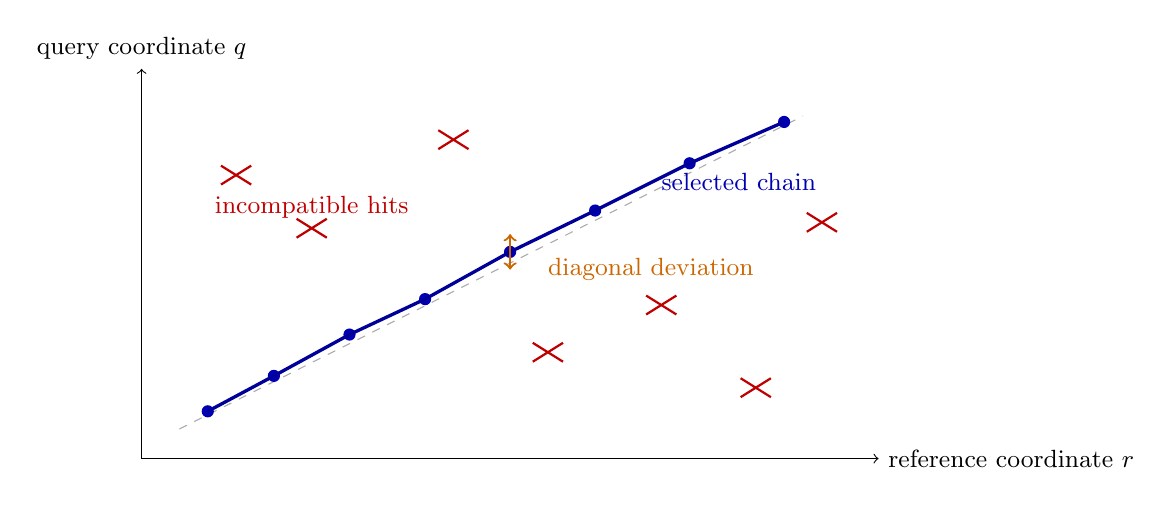
\begin{tikzpicture}[x=0.12cm,y=0.075cm,font=\small]
  \draw[->] (0,0) -- (78,0) node[right] {reference coordinate \(r\)};
  \draw[->] (0,0) -- (0,66) node[above] {query coordinate \(q\)};
  \draw[dashed,gray!65] (4,5) -- (70,58);
  \foreach \x/\y in {7/8,14/14,22/21,30/27,39/35,48/42,58/50,68/57}
    \fill[blue!70!black] (\x,\y) circle (2.2pt);
  \draw[very thick,blue!60!black]
    (7,8)--(14,14)--(22,21)--(30,27)--(39,35)--(48,42)--(58,50)--(68,57);
  \foreach \x/\y in {10/48,18/39,33/54,43/18,55/26,65/12,72/40}
    \draw[red!75!black,thick] (\x-1.6,\y-1.6)--(\x+1.6,\y+1.6)
      (\x-1.6,\y+1.6)--(\x+1.6,\y-1.6);
  \draw[<->,orange!80!black,thick] (39,32) -- (39,38);
  \node[orange!80!black,anchor=west] at (42,32)
    {diagonal deviation};
  \node[blue!70!black,below right] at (54,50) {selected chain};
  \node[red!75!black,above] at (18,39) {incompatible hits};
\end{tikzpicture}
\caption{Chaining selects growing, approximately
collinear path so we can get closer to the final result. Base-level alignment (later stage of the pipeline) will later resolve gaps between anchors.}
\label{fig:chaining-dotplot}
\end{figure}

\info{Why we look for anchors that are colinear?}{In the perfect scenario without gaps \(r_i-q_i\) is constant. An increasing diagonal coordinate indicates that in reference we matched more symbols than in the query (meaning insertion/deletion has occured). Chaining needs to specify costs for abandoning the main diagonal too much (intuitevely we don't want the case in which we introduce very large gap in the reference sequence just to match one or two symbols in the query, because it's improbable that some very large fragment was replaced during evolutionary processes by just a few bases)}

As we would like to have some well defined order of anchors, we sort them by strand and reference coordinate first, then by the additional metadata:
\begin{equation}
\begin{split}
 K_r(a_i) &=
   (\sigma_i \ll 63)\mathbin{\vert}
   \bigl(r_i\mathbin{\&}(2^{63}-1)\bigr),\\
 K_q(a_i) &=
   (g_i\ll48)\mathbin{\vert}(\phi_i\ll40)
   \mathbin{\vert}(\ell_i\ll32)
   \mathbin{\vert}(q_i\bmod 2^{32}).
\end{split}
\label{eq:chaining-order}
\end{equation}

Comparison is lexicographic in \(K_r\), \(K_q\), and the full \(q_i\). The hashing doesn't need full 64 bits for query position i.e if query coordinates $q_i$ exceed \(2^{32}\) we still have correct order as the leftmostpart is still the fragment number $g_i$ (fragments won't be larger than $2^{32}$). Fragmentation of sequences is discussed later in the storage chapter.

The ordering is required, because the chaining wants to process anchors in sequential order (increasing query positions), while we build chains of anchors using reference positions.

\section{Chaining components}

We defined the anchors that are input to chaining pipeline stage, however chaining itself isn't a monolith. It can be viewed as composition of several steps. 

\info{Chaining pipeline}{Although chaining can be decomposed into several steps that are dispatched to differrent functions, in BioseqDB this is an internal implementation detail and we don't allow users to alter for example which backtracking backend is used (although we could expose parts of chaining as composable components in the future)}

Forward chaining (which is the core component) produces the score array \(f\) and predecessor array \(p\). Second most important step is backtracking (as typically in case of DP algorithms which fill some state matrices) reads the sorted anchors, \(f\), and \(p\). The backtracking writes theflat output
anchor array supplied by the caller, denoted by \(A\) ($A$ can be viewed as type \texttt{anchor A\[\]}).

The chaining can be fully decomposed into the following steps:
\begin{enumerate}
  \item \textbf{Forward chaining} reads the sorted anchors and writes the
    temporary \(f\) and \(p\) arrays.
  \item \textbf{Backtracking} reads these inputs and writes the accepted chain
    records plus full anchor copies in \(A\).
  \item \textbf{Region generation} converts each chain record into one
    alignment region while retaining \(A\).
  \item \textbf{Region selection} filters the regions while
    retaining \(A\).
  \item \textbf{Base-level alignment} reads the selected regions, their slices
    of \(A\), the query and target sequences, and the alignment parameters. It
    fills the base-level fields in the regions supplying exact start/end coordinates, match qualities etc.
\end{enumerate}

BioseqDB represents every chain record with the following structure:
\begin{BioseqCppSnippet}
  struct chain {
    int32_t score        = 0;    (*@\BioseqCodeNote{Accepted-chain score}@*)
    int32_t anchor_count = 0;    (*@\BioseqCodeNote{Anchors in the chain}@*)
    int32_t anchor_start = 0;    (*@\BioseqCodeNote{Start of the chain slice in A}@*)
  };
\end{BioseqCppSnippet}
Where \texttt{anchor\_start} is the index of the first anchor in the chain in the array \(A\).

For a non-empty
record \(c\), its anchors occupy consecutive positions in forward order:
\[
  A[c.\texttt{anchor\_start}],\ldots,
  A[c.\texttt{anchor\_start}+c.\texttt{anchor\_count}-1].
\]

The array \(A\) is constructed using $f$ and $p$ arrays. For every anchor \(i\), the two stored values mean:
\begin{description}
  \item[\(f_i\)] the score of the best chain that the selected forward
    algorithm found with anchor \(i\) at its end.
  \item[\(p_i\)] the index of the anchor immediately before \(i\) in that
    chain. The value is \(-1\) when the best chain found for \(i\) starts at
    \(i\)
\end{description}
For example,
\[
  p_7=5,\qquad p_5=2,\qquad p_2=-1
  \quad\Longrightarrow\quad
  7\to5\to2\to-1.
\]

\raggedbottom

\definecolor{chainGray}{HTML}{A0A0A0}
\definecolor{chainBlue}{HTML}{4C78A8}
\definecolor{chainOrange}{HTML}{F28E2B}
\definecolor{chainGreen}{HTML}{59A14F}
\tikzset{
  chain stage/.style={draw=black!65,fill=gray!7,rounded corners,
    align=center,minimum height=.78cm,inner sep=4pt},
  chain blue/.style={chain stage,draw=chainBlue!90!black,fill=chainBlue!11},
  chain orange/.style={chain stage,draw=chainOrange!90!black,fill=chainOrange!14},
  chain green/.style={chain stage,draw=chainGreen!80!black,fill=chainGreen!12},
  chain muted/.style={chain stage,draw=chainGray!85!black,fill=chainGray!12},
  chain flow/.style={-{Latex[length=1.8mm]},thick},
  chain soft flow/.style={-{Latex[length=1.6mm]},thick,draw=chainGray!90!black},
  chain point/.style={circle,draw=chainBlue!90!black,fill=chainBlue!18,
    minimum size=.38cm,inner sep=0pt},
  chain current/.style={circle,draw=chainOrange!95!black,very thick,
    fill=chainOrange!20,minimum size=.48cm,inner sep=0pt}
}

\section{Chaining algorithms}
\label{sec:chaining-algorithm-families}

Similar to the minimizer chapter here we will discuss different approaches to chaining. The algorithm itself is based on dynamic programming scoring, but the details differ.

\begin{table}[H]
\centering
\caption{Comparison of different chaining algorithms}
\label{tab:chaining-algorithm-taxonomy}
\footnotesize
\setlength{\tabcolsep}{3.2pt}
\renewcommand{\arraystretch}{1.10}
\begin{tabularx}{\linewidth}{@{}
  >{\raggedright\arraybackslash}p{0.07\linewidth}
  >{\raggedright\arraybackslash}p{0.23\linewidth}
  >{\raggedright\arraybackslash}X
  >{\raggedright\arraybackslash}p{0.26\linewidth}@{}}
\toprule
\textbf{ID} & \textbf{Algorithm} & \textbf{Defining decision} &
\textbf{Implementations}\\
\midrule
B1 & Ordered predecessor scan & Visit recent candidates first. Increase the
skip counter when a marked candidate does not improve the score. Decrease a
positive counter after an improvement. Stop when the counter exceeds its
limit. Also score cached predecessor \(m\) when it exists and the main scan
does not reach it
& minimap2 non-RMQ chaining, BioSeqDB scalar and exact SIMD\\
B2 & Source-to-target DP & Apply each completed source score in parallel
to later targets admitted by the kernel's index and distance checks
& G3SA first CUDA pass\\
B3 & Ranking-value second pass & Rank predecessors by a value calculated from
their saved scores and coordinates. Keep at most one predecessor with the
largest accepted ranking value. If one was saved, calculate its full pair
score & G3SA second CUDA pass\\
B4 & Range-minimum-query tree DP & Use a balanced tree whose nodes cache the
smallest stored priority in each subtree, then calculate the full score for the
selected predecessor & minimap2 RMQ and BioSeqDB's experimental RMQ route,
which includes both query-coordinate boundaries and omits the bandwidth check\\
B5 & Per-element batch-limited DP & Keep one running score for each vector
element. Stop after enough consecutive batches leave all of those scores unchanged &
BioSeqDB bounded CPU SIMD\\
B6 & Per-target batch-limited DP & Keep one best score for the target.
Stop after enough consecutive batches fail to increase that score & BioSeqDB Vulkan\\
\bottomrule
\end{tabularx}
\end{table}

Scalar and exact SIMD both implement B1 because they make the same ordered
decisions. G3SA selects a short kernel or one of two tiled launch
configurations according to range size within B2 and B3. BioSeqDB CPU SIMD and
Vulkan use different batch stopping rules, so they are B5 and B6.

All implementations pass their saved scores and predecessors to later code
that builds and classifies mappings.

The BioSeqDB RMQ implementation includes both query-coordinate boundaries. It can
select a predecessor with the same query coordinate as the target and accept
it without a bandwidth test. We classify the tree design as B4 and describe
these defects in
Section~\ref{sec:chaining-bioseqdb}.

\subsection{Shared pair score}

Let's say we have two anchors with coordinates $q_j, q_i$ and $r_j, r_i$ on the query and reference.
Let's assume the minimizer span is always $k$. We now can say that after incorporating $(r_j, r_i)$ anchor we will cover $q_i-q_j$ symbols on the query and $r_i-r_j$ symbols on the reference, however those two jumps can be interpreted as
taking some symbols from query and assuming they form replacement and the rest forms a gap. For example let's say $q_i-q_j > r_i-r_j$. This means that we match more symbols in query than in reference, so indicates some deletion in the reference.
So we can say $r_i-r_j$ symbols are replaced (or stay the same) while the leftover $(q_i-q_j)-(r_i-r_j)$ symbols form this deletion. This thinking is symmetrical so we just only need to use minimum and absolute value to make it more generic.

Now we introduced $g(j,i)$ (the advance shared by the reference and query) and $\delta(j,i)$ (the remaining advance in whichever sequence moves farther).
As k-mers represent hashed fragment of length $k$ we can assume that in our match we have exactly $\min\{q_i-q_j, r_i-r_j, k\}$ new symbols that matched.
Hence we now define our first primitive score as $\min\{q_i-q_j, r_i-r_j, k\} = \min\{g(j,i), k\}$.

This scoring has some problems with the most important one being that it doesn't penalize the case when we have a large gap in the reference sequence just to match one or two symbols in the query. This is improbable that some very large fragment was replaced during evolutionary processes by just a few bases.
For that reason we will use function $\left\lfloor\text{Penalty}(\delta, g)\right\rfloor$. The penalty function should satisfy the following properties:
\begin{itemize}
  \item There's no penalty for doing nothing at all: $\text{Penalty}(0, 0) = 0$
  \item For $g \leq k \land \delta = 0$ there's no gap so there's shouldn't be any penalty: $\text{Penalty}(0, g) = 0$
  \item Penalty should be monotonically increasing with respect to $\delta$: $\text{Penalty}(\delta, g) \leq \text{Penalty}(\delta+1, g)$
  \item Penalty should be increasing slower than linearly with respect to $g$: $\text{Penalty}(\delta, g+1) < \text{Penalty}(\delta, g) + 1$. This guarantees that increasing $g$ without touching $\delta$ benefits overall score (we prefer replacement region over gap region)
  \item For small $g$ and $\delta$ our penalty function should prefer increase in $g$ rather than $\delta$. This is equivalent of saying that we want to stay close to the diagonal and reduce the gap size introduced: $\text{Penalty}(\delta+1, g) \geq \text{Penalty}(\delta, g+1)$
  \item For large $g$ and $\delta$ our penalty function should be asymptotically the same for both $\delta$ and $g$. This is equivalent of saying that if we encounter very large gaps, then it doesn't matter if we increase the matching region between two fragments or increase the gap as both fragments are very dissimilar: $O_{\delta}(\text{Penalty}(\delta, g = \text{const})) = O_{g}(\text{Penalty}(\delta = \text{const}, g))$
\end{itemize}

\info{Symmetry}{Using $g$ and $\delta$ as only parameters for penalty function guarantees that scoring is symmetric. Symmetry makes sure that gap costs are the same for both query and reference.}

Our final score is then something of the following structure:
\begin{equation}
\begin{gathered}
\text{Score}(j,i) = \min\{g(j,i), k\} - \left\lfloor\text{Penalty}(\delta(j,i), g(j,i))\right\rfloor \\
= \min\{g(j,i), k\} - \left\lfloor \alpha * g(j,i) + \beta * \delta(j,i) + \gamma * f(\delta(j,i)) \right\rfloor \\
0 \leq \alpha, \beta, \gamma \leq 1
\end{gathered}
\end{equation}

\begin{figure}[tbp]
\centering
\begin{tikzpicture}[x=.34cm,y=.34cm,font=\footnotesize,>=Latex,
  dist axis/.style={-{Latex[length=1.4mm]},thin},
  dist common/.style={-{Latex[length=1.7mm]},very thick,
    draw=chainGreen!80!black},
  dist excess/.style={-{Latex[length=1.7mm]},very thick,
    draw=chainOrange!95!black},
  dist measure/.style={<->,thin,draw=chainBlue!90!black},
  dist summary/.style={draw=black!55,fill=gray!4,rounded corners=0pt,
    text width=3.75cm,align=center,inner sep=3pt}]

  \begin{scope}[xshift=0cm]
    \node[font=\bfseries,align=center,text width=4.5cm] at (4.3,12.0)
      {(a) Both advances\\are below \(k\)};
    \draw[dist axis] (-.15,0)--(9.4,0) node[below right] {\(r\)};
    \draw[dist axis] (0,-.15)--(0,9.5) node[above left] {\(q\)};
    \node[chain point,label=below left:\(a_j\)] (d1j) at (0,0) {};
    \node[chain current,label=above right:\(a_i\)] (d1i) at (3,3) {};
    \draw[dist common] (d1j)--node[midway,above left] {\(g=3\)} (d1i);
    \node[text=chainOrange!95!black,anchor=west] at (3.8,3.0)
      {\(\delta=0\)};
    \draw[dist measure] (0,-1.05)--node[midway,below] {\(d_r=3\)}
      (3,-1.05);
    \draw[dist measure] (-1.05,0)--node[midway,left] {\(d_q=3\)}
      (-1.05,3);
    \node[dist summary] at (4.25,-4.6)
      {\(g=3,\ \delta=0\)\\reward \(\min(g,k)=3\)};
  \end{scope}

  \begin{scope}[xshift=5.0cm]
    \node[font=\bfseries,align=center,text width=4.5cm] at (4.3,12.0)
      {(b) Reference moves\\much farther};
    \draw[dist axis] (-.15,0)--(9.4,0) node[below right] {\(r\)};
    \draw[dist axis] (0,-.15)--(0,9.5) node[above left] {\(q\)};
    \node[chain point,label=below left:\(a_j\)] (d2j) at (0,0) {};
    \coordinate (d2g) at (2,2);
    \node[chain current,label=above right:\(a_i\)] (d2i) at (8,2) {};
    \draw[dist common] (d2j)--node[midway,above left] {\(g=2\)} (d2g);
    \draw[dist excess] (d2g)--node[midway,above] {\(\delta=6\)} (d2i);
    \draw[dist measure] (0,-1.05)--node[midway,below] {\(d_r=8\)}
      (8,-1.05);
    \draw[dist measure] (-1.05,0)--node[midway,left] {\(d_q=2\)}
      (-1.05,2);
    \node[dist summary] at (4.25,-4.6)
      {\(g=2,\ \delta=6\)\\reward \(\min(g,k)=2\)};
  \end{scope}

  \begin{scope}[xshift=10.0cm]
    \node[font=\bfseries,align=center,text width=4.5cm] at (4.3,12.0)
      {(c) Both advances\\exceed \(k\)};
    \draw[dist axis] (-.15,0)--(9.4,0) node[below right] {\(r\)};
    \draw[dist axis] (0,-.15)--(0,9.5) node[above left] {\(q\)};
    \node[chain point,label=below left:\(a_j\)] (d3j) at (0,0) {};
    \coordinate (d3g) at (7,7);
    \node[chain current,label=above right:\(a_i\)] (d3i) at (8,7) {};
    \draw[dist common] (d3j)--node[midway,above left] {\(g=7\)} (d3g);
    \draw[dist excess] (d3g)--node[midway,below] {\(\delta=1\)} (d3i);
    \draw[dist measure] (0,-1.05)--node[midway,below] {\(d_r=8\)}
      (8,-1.05);
    \draw[dist measure] (-1.05,0)--node[midway,left] {\(d_q=7\)}
      (-1.05,7);
    \node[dist summary] at (4.25,-4.6)
      {\(g=7,\ \delta=1\)\\reward \(\min(g,k)=5\)};
  \end{scope}
\end{tikzpicture}
\caption{Three anchor displacements for \(k=5\). The blue brackets are the
actual reference and query advances. The green diagonal step advances both
coordinates by \(g=\min(d_r,d_q)\). The orange horizontal step is the
remaining \(\delta=|d_r-d_q|\). It would be vertical when \(d_q>d_r\).
Panel (c) also shows that the reward stops at \(k\), even though \(g>k\).}
\label{fig:chaining-distance-examples}
\end{figure}

The minimap2 scoring definition $E$ looks exactly as what we have just specified:
\begin{equation}
\begin{aligned}
 d_q(j,i) &= q_i-q_j, & d_r(j,i) &= r_i-r_j,\\
 \delta(j,i) &= \lvert d_r(j,i)-d_q(j,i)\rvert,
 & g(j,i) &= \min\{d_r(j,i),d_q(j,i)\}.
\end{aligned}
\label{eq:chaining-distances}
\end{equation}

\begin{equation}
 E(j,i)=\min\{\ell_j,g(j,i)\}-P(j,i),
\label{eq:chaining-link-score}
\end{equation}
where
\begin{equation}
P(j,i)=
\begin{cases}
0,
  & \delta(j,i)=0\ \land\ g(j,i)\leq\ell_j,\\[2pt]
\left\lfloor
  \lambda_g\delta(j,i)+\lambda_s g(j,i)
  +\dfrac{1}{2}\operatorname{mglog}_{2}\!\bigl(\delta(j,i)+1\bigr)
\right\rfloor,
  & \text{otherwise}.
\end{cases}
\label{eq:chaining-penalty}
\end{equation}
The function \(\operatorname{mglog}_{2}\) is minimap2's polynomial
approximation of \(\log_2\). So far in the abstract definition of scoring we didn't mention diagonal, but nonnegative coefficient \(\lambda_g\) can be viewed as diagonal-gap penalty (further away from diagonal we penalize more), where the nonnegative coefficient \(\lambda_s\) is the penalty for distance. The value \(\ell_j\) is the
query span of predecessor \(j\). (In our example above we used $k$ for all k-mers sizes, but as mentioned before minimap2 with specific settings can compress regions of same repeating symbols so we just replace $k$ with kmer span $\ell_j$. All the logic stays the same) \coderef{minimap2/lchain.c}
{Minimap2 chaining link score}{comput_sc}{113}

\info{Score units}{In this definition we view scoring function as expressed in number of matched symbols (not some arbitrary large numbers), so the coefficients must be set accordingly so the values are scaled correctly. In the dynamic programming formulation we then can take maximum of $E$ value and $\ell_i$ to make sure that in the worst case scenario we assume that we at least matched the length of the minimizer. There are no formal limitations on this normalization, but it makes reasoning about the scores easier.}

It's worth noting that defined scoring is also symmetrical in terms of coordinates i.e the score doesn't take $r_i, q_i$ positions as parameters so reversing coordinate systems doesn't change the outcome.
However, in dynamic programming we often want to use the locally close predecessor as the best one. 
Consider for example situation in which we have two possible candidates for some anchor $i$: one is very close to our position while offering lower cummulative score for the chain, while the other one is very far away but offers high cummulative score. This scenario can happen if we have very good chain with narrow gaps and slightly worse chain with larger gaps, but the two are very far away from current position.
We can have selection function that not only takes the best score, but also adds function dependent on current anchor position to make sure to formally express that preference:
\begin{equation}
\begin{aligned}
  f_j = \max_{i < j}\{f_i+E(j,i)\}, \\
  \text{Selection}(i) &= f_j + \phi(r_i, q_i)
\end{aligned}
\end{equation}

There shouldn't be any difference in behaviour for query and reference so $\phi$ should be symmetric. Additionally $\phi$ should be monotonic to express the fact that we prefer closer predecessors: $\phi(r_i, q_i) \leq \phi(r_i+1, q_i), \phi(r_i, q_i+1) \leq \phi(r_i+1, q_i+1)$.
Please note that the difference here is that it's not a cummulative chain score. It's only used to select the best predeccesor for current anchor (if we tried to sum this score up we would get total score having $O(n^2)$ terms, which would severly alter the scoring behaviour discussed earlier).

In the later chapters we discuss selection function that uses artithmetical average of positions:
\begin{equation}
\begin{aligned}
  \operatorname{Selection}(j) = f_j+\phi(r_i, q_i) \\
  \phi(r_i, q_i) = \frac{r_i + q_i}{2}
\end{aligned}
\end{equation}

\begin{figure}[tbp]
\centering
\begin{tikzpicture}[x=.38cm,y=.38cm,font=\footnotesize,>=Latex,
  link axis/.style={-{Latex[length=1.4mm]},thin},
  link path/.style={-{Latex[length=1.8mm]},very thick,
    draw=chainGreen!80!black},
  link measure/.style={<->,thin,draw=chainBlue!90!black},
  link summary/.style={draw=black!55,fill=gray!4,rounded corners=0pt,
    text width=5.0cm,align=center,inner sep=3pt}]

  \begin{scope}[xshift=0cm]
    \node[font=\bfseries] at (5.0,11.0) {(a) Close predecessor};
    \draw[link axis] (-.15,0)--(11.0,0) node[below right] {reference \(r\)};
    \draw[link axis] (0,-.15)--(0,10.2) node[above left] {query \(q\)};
    \draw[dashed,draw=chainGray!80!black] (1,0)--(11,10);
    \node[chain point,label={left:\(a_{j_{\mathrm{near}}}=(7,6)\)}]
      (nearj) at (7,6) {};
    \node[chain current,label={above right:\(a_i=(10,9)\)}]
      (neari) at (10,9) {};
    \draw[link path] (nearj)--node[midway,above left] {\(g=3\)}
      (neari);
    \draw[link measure] (7,-1.0)--node[midway,below] {\(d_r=3\)}
      (10,-1.0);
    \draw[link measure] (10.75,6)--node[midway,right] {\(d_q=3\)}
      (10.75,9);
    \node[link summary] at (5.0,-4.5)
      {same diagonal: \(\delta=0\)\\link advances 3 positions in each sequence};
  \end{scope}

  \begin{scope}[xshift=7.6cm]
    \node[font=\bfseries] at (5.0,11.0) {(b) Far predecessor};
    \draw[link axis] (-.15,0)--(11.0,0) node[below right] {reference \(r\)};
    \draw[link axis] (0,-.15)--(0,10.2) node[above left] {query \(q\)};
    \draw[dashed,draw=chainGray!80!black] (1,0)--(11,10);
    \node[chain point,label={above left:\(a_{j_{\mathrm{far}}}=(2,1)\)}]
      (farj) at (2,1) {};
    \node[chain current,label={above right:\(a_i=(10,9)\)}]
      (fari) at (10,9) {};
    \draw[link path] (farj)--node[midway,above left] {\(g=8\)}
      (fari);
    \draw[link measure] (2,-1.0)--node[midway,below] {\(d_r=8\)}
      (10,-1.0);
    \draw[link measure] (10.75,1)--node[midway,right] {\(d_q=8\)}
      (10.75,9);
    \node[link summary] at (5.0,-4.5)
      {same diagonal: \(\delta=0\)\\link advances 8 positions in each sequence};
  \end{scope}
\end{tikzpicture}
\caption{A close and a far predecessor for the same current anchor
\(a_i=(10,9)\). Both candidates lie on the diagonal \(r-q=1\), so both have
\(\delta=0\). Their link lengths are nevertheless different: the close link
has \(g=3\), whereas the far link has \(g=8\). Thus zero diagonal deviation
does not mean zero or equal distance.}
\label{fig:chaining-near-far-distance}
\end{figure}

\info{Selection}{Adding the term with the coordinate's average can be interpretes as requirement that the chain score should increase linearly with the distance between the current anchor and the selected predecessor. If some chain is twice far away than other then it should offer at least twice better score. There are many otehr functions that could be placed here as $\phi$, but simple average is the simplest one}

\section{B1: minimap2 dynamic programming}
\label{sec:chaining-b1}

As our scoring model $E(i,j)$ depends only on two anchors we can define recursive equations for dynamic programming:
\begin{equation}
 f_i=\max\!\left(
   \ell_i,
   \max_{j\in\mathcal{C}_i}\{f_j+E(j,i)\}
 \right),
 \qquad
 p_i=\operatorname*{arg\,max}_{j\in\mathcal{C}_i}\{f_j+E(j,i)\}.
\label{eq:chaining-b1-recurrence}
\end{equation}
Where $\mathcal{C}_i$ is the set of valid predecessors (selected by being close to diagonal - this is form of specifying cutoff condition so we don't need to check all possible predecessors all the time).
Maximum function is used here to make sure that in worst case if our definition of $E(i,j)$ yield very low score we can say that we matched at least length of the minimizer span.

If no predecessor improves the base value of score \(\ell_i\), then
\(p_i=-1\).

We will call iteration over $\mathcal{C}_i$ a scan. Minimap2 does this scan by visiting anchors in order from newest to oldest.

After sorting, minimap2 numbers the anchors \(0,1,\ldots,n-1\). When the DP algorithm
reaches anchor \(i\), the scores \(f_0,\ldots,f_{i-1}\) and predecessor
indices \(p_0,\ldots,p_{i-1}\) have already been calculated. It starts a new
chain at \(i\) with
\[
  f_i=\ell_i \qquad\text{and}\qquad p_i=-1,
\]
Minimap2 tests earlier anchors in the order \(j=i-1,i-2,\ldots\) (larger
index is tested first). For every pair that passes the distance checks, it
calculates
\[
  c_j=f_j+E(j,i).
\]
If \(c_j>f_i\), anchor \(j\) becomes the new predecessor:
\(f_i\gets c_j\) and \(p_i\gets j\) (strict equality is important here so we avoid using older anchors with the same score)

Trying every earlier anchor would make this dynamic program expensive. Minimap2 applies the following strategies to limit the work performed:
\begin{itemize}
  \item \texttt{max\_iter} limits how many previous anchors we scan: this is the number of highest-numbered array positions before \(i\).
  \item \texttt{max\_skip} is the limit on skip counter \(s\). It starts at zero for every new \(i\) and is increased by one on marked anchor that fails to improve the score and decreased by one on marked anchor that improves the score. If skip counter exceeds limit we finish scan loop early and do not scan other previous anchors.
  \item \texttt{m} is an extra candidate that is tested after the scan loop. It is the anchor with the highest score among all previously tested anchors (this is a measure to prevent skipping good chains due to too aggressive skip counter limit)
  \item \texttt{CanScore(j,i)} checks the anchor distances to make sure the anchor lies within the band (close to diagonal). It uses $D_x$ and $D_y$ for limits on reference and query distances respectively and $B$ for distance from diagonal.
\end{itemize}

Minimap2 contains separate rules for multi-segment and cDNA input. The key algorithm stays the same and differences are very subtle:
\begin{itemize}
  \item There are differences in handling scoring case of \(g_i=g_j\)
  \item Multi-segment non-cDNA input adds special requirement \(d_r\leq D_y\)
  \item cDNA input does not force \(D_y\geq B\)
  \item There are differences in penatly factors for scoring function $E(j,i)$
\end{itemize}

In description below I assume we talk about default case of one-segment, non-cDNA input.

\info{Different kinds of input}{Multi-segment input is in case of Minimap2 described as a situation in which single query maps to different fragments of the reference section. I do not support this use case in BioseqDB out of the box at this time. This situation is also known as split-read or supplementary alignment and normally occurs due to due to structural variations, translocations, or chimeric artifacts in the genome. cDNA in this case describes the same situation, but has slightly different scoring parameters. Even though that can be interesting, we don't want to describe these modes here since those are very specialized heuristics}

\subsection{Skipping with counters and marked anchors}

As discussed above minimap2 scores only valid pairs of anchors:
\begin{equation}
  0<d_r(j,i)\leq D_x,\qquad
  0<d_q(j,i)\leq\min(D_x,D_y),\qquad
  \delta(j,i)\leq B,
  \label{eq:chaining-b1-pair-checks}
\end{equation}
where \(B=\texttt{bw}\) where all parameters like $\texttt{bw}$ are minimap2's CLI arguments.
\[
  D_x=\max(\texttt{max\_dist\_x},B),\qquad
  D_y=\max(\texttt{max\_dist\_y},B).
\]

After a candidate \(j\) passes this checks, we calculate $E(i,j)$ score and then update $p_j$ if we see better score. We want to that $p_j$ was updated in scan for $i$. This can be understood as building chains in parallel where we want to save information about predecessor for each anchor:
\[
  t_{p_j}\gets i \qquad\text{when }p_j\geq0.
\]
If some time later in other scan we see that $t_{p_j}=i$ then we know that $p_j$ was updated in scan for $i$ (we already tested candidate with a larger anchor). If marked anchor \(x\)
fails to improve \(f_i\), then \(s\) increases by one. A failed unmarked anchor leaves \(s\) unchanged. An improvement subtracts one from a positive
\(s\). It does not necessarily reset the counter to zero. The loop stops only when
\(s>\texttt{max\_skip}\)

\info{Interpretation}{This marking with skip counter can be intuitevely understood as a situation in which we try to improve the best chain by adding new anchor. If repeatedly this chain fails to improve the score, we don't want to waste more time on it.}

We don't perform this marking when this is candidate thatraises \(s\) above
\texttt{max\_skip} (in that case we stop the scan loop early).

Minimap2 keeps the loop index in \(e\). If the skip
test stopped the loop while it was processing \(j\), then \(e=j\). $e$ is used to check if we can score anchor $m$ (if $m<e$ then we can).

\(m\) is additional index saved by minimap2 on the side, which we call the
\emph{saved high-score anchor}. The saved value is
an anchor index whose previously calculated \(f_m\) is large. If \(m\) is absent or has left the reference-distance window (is too far),
minimap2 first rebuilds it by finding the largest \(f_j\) in the current
\texttt{max\_iter} set.

This saved anchor can then remain saved after
\(m<i-\texttt{max\_iter}\). Each time we check $e<m$ (see if we already scored this anchor) and if not we calculate $E(m,i)$ and do update checks similar to other anchors.
$m$ is introduced to make sure to take into consideration anchor that could be potentially a little bit further away. Minimap2 doesn't use priority queue or list here, because chaining accuracy is already good enough and this approach is much simpler.

\begin{figure}[H]
\centering
\begin{tikzpicture}[x=.86cm,y=.78cm,font=\footnotesize,>=Latex,
  scan anchor/.style={circle,draw=black!70,very thick,minimum size=.62cm,
    inner sep=0pt,font=\bfseries},
  scan improve/.style={scan anchor,draw=chainOrange!95!black,
    fill=chainOrange!22},
  scan marked/.style={scan anchor,draw=chainBlue!95!black,
    fill=chainBlue!19},
  scan plain/.style={scan anchor,draw=chainGray!90!black,
    fill=chainGray!16},
  scan cache/.style={scan anchor,draw=chainGreen!85!black,
    fill=chainGreen!18},
  skip badge/.style={draw=black!65,fill=white,minimum width=.72cm,
    minimum height=.34cm,inner sep=1pt,font=\scriptsize},
  pred link/.style={-{Latex[length=1.6mm]},very thick,
    draw=chainOrange!90!black},
  square note/.style={draw=black!65,fill=gray!5,align=left,
    rounded corners=0pt,inner sep=4pt}]
  \node[anchor=west,font=\bfseries] at (.15,12.95)
    {(a) Which earlier anchors can be scored};
  \draw[->] (.65,6.65)--(6.25,6.65) node[right] {reference \(r\)};
  \draw[->] (.65,6.65)--(.65,11.75) node[above] {query \(q\)};
  \draw[draw=chainBlue!65,dashed,fill=chainBlue!5]
    (1.20,7.05) rectangle (5.35,11.15);
  \draw[dashed,chainOrange!85!black] (1.10,6.95)--(5.55,11.40);
  \draw[dashed,chainOrange!85!black] (1.10,7.65)--(4.85,11.40);
  \node[chain point,label=below left:\(a_0\)] at (1.55,7.55) {};
  \node[chain point,label=below:\(a_1\)] at (2.55,8.55) {};
  \node[chain point,label=below right:\(a_2\)] at (3.70,9.10) {};
  \node[chain current,label=above right:\(a_i\)] at (5.35,11.15) {};
  \node[circle,draw=chainGray!90,fill=chainGray!15,minimum size=.35cm,
    inner sep=0pt,label={[align=right]left:{outside\\reference window}}]
    at (.88,7.02) {};
  \draw[chainOrange!90!black,very thick]
    (4.03,7.72)--(4.31,8.00) (4.03,8.00)--(4.31,7.72);
  \node[anchor=west,text=chainOrange!90!black] at (4.38,7.86)
    {outside band};
  \node[anchor=west,text=chainBlue!85!black] at (1.25,11.45)
    {distance limits};

  \node[square note,text width=5.45cm,anchor=west] at (7.35,9.35)
    {For one query segment, score \(j\) only if\\[2pt]
     \(a_j,a_i\) use the same reference and strand,\\
     \(0<d_r\leq D_x\),\\
     \(0<d_q\leq\min(D_x,D_y)\), and\\
     \(\lvert d_r-d_q\rvert\leq B\).};

  \node[anchor=west,font=\bfseries] at (.15,6.15)
    {(b) One complete backward scan with concrete counter values};
  \node[square note,text width=1.35cm,align=center] at (.85,2.75)
    {current \(i=8\)\\start \(f_8=8\)\\\(p_8=-1\)\\saved \(m=0\)};
  \draw[decorate,decoration={brace,amplitude=3pt}]
    (1.72,5.25)--(11.40,5.25)
    node[midway,above=4pt]
      {main loop: positions 7 through 1
       (\texttt{max\_iter}\(=7\))};

  \node[scan improve] (s7) at (2.10,3.72) {7};
  \node[scan plain]   (s6) at (3.60,1.78) {6};
  \node[scan marked]  (s5) at (5.10,3.72) {5};
  \node[scan marked]  (s4) at (6.60,1.78) {4};
  \node[scan improve] (s3) at (8.10,3.72) {3};
  \node[scan marked]  (s2) at (9.60,1.78) {2};
  \node[scan marked]  (s1) at (11.10,3.72) {1};
  \node[scan cache]   (s0) at (12.60,1.78) {0};

  \draw[pred link] (s7.east)--node[midway,above,font=\scriptsize]
    {\(p_7=5\)} (s5.west);
  \draw[pred link] (s5.east)--node[midway,above,font=\scriptsize]
    {\(p_5=3\)} (s3.west);
  \draw[pred link] (s3.east)--node[midway,above,font=\scriptsize]
    {\(p_3=1\)} (s1.west);
  \draw[pred link] (s6.east)--node[midway,below,font=\scriptsize]
    {\(p_6=4\)} (s4.west);
  \draw[pred link] (s4.east)--node[midway,below,font=\scriptsize]
    {\(p_4=2\)} (s2.west);
  \draw[pred link] (s2.east)--node[midway,below,font=\scriptsize]
    {\(p_2=0\)} (s0.west);

  \node[align=center,font=\scriptsize] at (2.10,4.52)
    {step 1\\\(c_7=14>8\)};
  \node[align=center,font=\scriptsize] at (5.10,4.52)
    {step 3\\\(c_5=12<14\)};
  \node[align=center,font=\scriptsize] at (8.10,4.52)
    {step 5\\\(c_3=16>14\)};
  \node[align=center,font=\scriptsize] at (11.10,4.52)
    {step 7\\\(c_1=14<16\): stop};

  \node[align=center,font=\scriptsize] at (3.60,.62)
    {step 2\\\(c_6=13<14\)};
  \node[align=center,font=\scriptsize] at (6.60,.62)
    {step 4\\\(c_4=11<14\)};
  \node[align=center,font=\scriptsize] at (9.60,.62)
    {step 6\\\(c_2=15<16\)};
  \node[align=center,font=\scriptsize,text=chainGreen!60!black] at (12.60,.62)
    {saved \(m=0\)\\\(c_0=17>16\)};

  \node[skip badge] at (2.47,3.34) {\(s=0\)};
  \node[skip badge] at (3.97,2.16) {\(s=0\)};
  \node[skip badge] at (5.47,3.34) {\(s=1\)};
  \node[skip badge] at (6.97,2.16) {\(s=2\)};
  \node[skip badge] at (8.47,3.34) {\(s=1\)};
  \node[skip badge] at (9.97,2.16) {\(s=2\)};
  \node[skip badge] at (11.47,3.34) {\(s=3\)};

  \node[square note,draw=chainGreen!75!black,fill=chainGreen!8,
    text width=1.55cm,align=center] (cacheout) at (14.38,2.72)
    {after checking \((0,8)\)\\\(f_8=17\)\\\(p_8=0\)};
  \draw[-{Latex[length=1.7mm]},very thick,draw=chainGreen!75!black]
    (s0.east)--(cacheout.west);

  \node[scan improve,minimum size=.38cm] at (1.05,-.38) {};
  \node[anchor=west,font=\scriptsize] at (1.30,-.38) {improves};
  \node[scan marked,minimum size=.38cm] at (3.25,-.38) {};
  \node[anchor=west,font=\scriptsize] at (3.50,-.38) {marked failure};
  \node[scan plain,minimum size=.38cm] at (6.25,-.38) {};
  \node[anchor=west,font=\scriptsize] at (6.50,-.38) {unmarked failure};
  \node[scan cache,minimum size=.38cm] at (9.65,-.38) {};
  \node[anchor=west,font=\scriptsize] at (9.90,-.38)
    {saved high-score anchor};
\end{tikzpicture}
\caption{(a) The reference and query limits and diagonal band decide whether a pair can be
scored or not. (b) If distance checks pass, then we perform scans in a loop. The picture shows one pass of the scan for the current anchor $i=8$. The numbers inside the circles are anchor indices. The orange
arrow from \(j\) to \(p_j\) shows the predecessor previously saved for anchor
\(j\). After \(j\) is scored without stopping, the arrow's destination
receives the current mark \(i=8\). The numbered steps visit anchors
\(7,6,\ldots,1\). The small \(s\) boxes show the single skip counter for
current anchor 8. Step 2 doesn't affect \(s\) as this anchor doesn't have a predecessor in this scan pass (it's unmarked). Step 5 improves the score and changes \(s=2\) to \(s=1\).
Anchor 0 is already outside the main loop because
\(\texttt{max\_iter}=7\), so we don't scan it, but we check it later with $m=0$. Step 7 stops with \(e=1\), so saved \(m=0\)
satisfies \(m<e\) and is checked once. The score of $m=0$ equal to 17 wins, but in some other scan other anchor could have a better score.}
\label{fig:chaining-b1-scan}
\end{figure}

\begin{algorithm}[H]
\caption{Minimap2's ordered predecessor scan for one query segment}
\label{alg:chaining-b1}
\small
\begin{algorithmic}[1]
  \Require sorted anchors \(a_0,\ldots,a_{n-1}\); ordinary non-cDNA mode;
           configured distance limits, \(B=\texttt{bw}\),
           \texttt{max\_iter}, and \texttt{max\_skip}
  \Ensure chain scores \(f_i\) and predecessor indices \(p_i\)
  \State \(D_x\gets\max(\texttt{max\_dist\_x},B)\)
  \State \(D_y\gets\max(\texttt{max\_dist\_y},B)\)
  \Function{CanScore}{\(j,i\)}
    \State \(d_q\gets q_i-q_j,\quad d_r\gets r_i-r_j\)
    \If{\(a_j,a_i\) use different references or strands}
      \State \Return false
    \EndIf
    \If{\(d_r\leq0\) \textbf{or} \(d_r>D_x\)}
      \State \Return false
    \EndIf
    \If{\(d_q\leq0\) \textbf{or} \(d_q>D_x\) \textbf{or} \(d_q>D_y\)}
      \State \Return false
    \EndIf
    \If{\(\lvert d_r-d_q\rvert>B\)}
      \State \Return false
    \EndIf
    \State \Return true
  \EndFunction
  \State \(t_j\gets0\) for every \(j\); \(m\gets-1\); \(st\gets0\)
        \Comment{\(m\) is one saved anchor index}
  \For{\(i\gets0\) \textbf{to} \(n-1\)}
    \While{\(st<i\) and
      (\(a_{st}\) has a different reference or strand from \(a_i\), or
       \(r_i-r_{st}>D_x\))}
      \State \(st\gets st+1\)
    \EndWhile
    \State \(st\gets\max(st,i-\texttt{max\_iter})\)
          \Comment{hard lower bound for the main scan}
    \State \(f_i\gets\ell_i,\quad p_i\gets-1,\quad s\gets0,\quad
            e\gets st-1\)
    \For{\(j\gets i-1\) \textbf{down to} \(st\)}
      \If{\Call{CanScore}{\(j,i\)}}
        \State \(c\gets f_j+E(j,i)\)
        \If{\(c>f_i\)}
          \State \(f_i\gets c,\quad p_i\gets j\)
          \If{\(s>0\)}
            \State \(s\gets s-1\)
          \EndIf
        \ElsIf{\(t_j=i\)}
          \State \(s\gets s+1\)
          \If{\(s>\texttt{max\_skip}\)}
            \State \(e\gets j\)
            \State \textbf{break}
          \EndIf
        \EndIf
        \If{\(p_j\geq0\)}
          \State \(t_{p_j}\gets i\)
              \Comment{mark one older anchor for this scan}
        \EndIf
      \EndIf
    \EndFor
    \If{\(m<0\), or \(a_m\) has a different reference or strand from \(a_i\),
          or \(r_i-r_m>D_x\)}
      \State \(m\gets-1\)
      \For{\(j\gets i-1\) \textbf{down to} \(st\)}
        \If{\(m<0\) \textbf{or} \(f_j>f_m\)}
          \State \(m\gets j\)
        \EndIf
      \EndFor
    \EndIf
    \If{\(m\geq0\) and \(m<e\)}
      \If{\Call{CanScore}{\(m,i\)}}
        \State \(c\gets f_m+E(m,i)\)
        \If{\(c>f_i\)}
          \State \(f_i\gets c,\quad p_i\gets m\)
        \EndIf
      \EndIf
    \EndIf
    \If{\(m<0\), or (\(a_m,a_i\) use the same reference and strand,
          \(r_i-r_m\leq D_x\), and \(f_i>f_m\))}
      \State \(m\gets i\)
    \EndIf
  \EndFor
\end{algorithmic}
\end{algorithm}

\info{Algorithm details}{We check if \(a_{st}\) has a different reference or strand from \(a_i\), because anchors in minimap2 can originate from different refences. In BioseqDB this won't happen, but we still need to check for strand direction. Also please note that formally we use different values for marking $t_{p_j} \gets i$, but it's main goal is just to detect visited anchors for the same scan pass (like in binary map, but assigning $i$ just means that we don't have to clear it.)}


\section{BioseqDB SIMD DP: exact and bounded batch}
\label{sec:chaining-simd-forward}

For one target anchor \(a_i\), scalar B1 tests possible predecessors one at a
time.  During the sacan it starts at \(a_{i-1}\) and walks towards the lower end of the search
window. SIMD implementations both implement the same outer loop, but the scan itself is rewritten: We place each predecessor candidate in batches of size $L$ (each batch is one SIMD vector) - one vector call can
calculate as many as \(L\) values of \(E(j,i)\). We have two kinds of SIMD algorithm:

\begin{enumerate}
  \item \textbf{Exact SIMD B1 called \texttt{exact\_visited}}
        It it the most naive implementation: it calculates up to \(L\) pair scores together in a SIMD vector, but \(F\), \(P\), and \(s\) are still single scalars as in original B1. 

  \item \textbf{Bounded batch SIMD B1 called
        \texttt{bounded\_batch\_}\allowbreak\texttt{approximate}.}
        Algorithm removes the mark array completely, while scalar skip counter in now counting batches.  Lane \(\lambda\)
        keeps its own temporary best score \(H_\lambda\) and predecessor
        \(P_\lambda\).  A shared counter \(u\) records how many
        batches in a row failed to improve any lane (the algorithm stops when \(u\)
        reaches its batch limit \(U\)). We take the largest score across the lane winners and test the saved
        anchor \(m\) once.
\end{enumerate}

We will discuss bounded batch SIMD B1 first, as it is more interesting one.

\subsection{Candidates in SIMD vectors}

The candidates are placed in batches. So now in loops we use \(b=0\) instead of $j$ where $0$ is the first batch, \(b=1\) is the next older
batch, and so on.  Within one batch,
\(\lambda\in\{0,\ldots,L-1\}\) is the SIMD lane number.  The candidate
placed in that lane is \(j_{b,\lambda}\).

First we introduce the most boring thing - coordinates mapping:
\begin{equation}
\begin{aligned}
  \mathrm{end}_b   &= i-bL,
  &\qquad \mathrm{begin}_b &= \max(st_i,\mathrm{end}_b-L),\\
  a_b              &= \mathrm{end}_b-\mathrm{begin}_b,
  &\qquad j_{b,\lambda} &= \mathrm{begin}_b+\lambda .
\end{aligned}
  \label{eq:chaining-simd-batch-map}
\end{equation}
Here \(\mathrm{end}_b\) is the position immediately after the batch,
\(\mathrm{begin}_b\) is its first candidate, and \(a_b\) is its number of
active lanes. As candidates are split into batches, the last one can be partial (so $a_b$ will be used to mask out the inactive lanes).

For lane \(\lambda\), the pair scorer first calculates
\(\epsilon_{b,\lambda}=E(j_{b,\lambda},i)\).  The code then loads the earlier
chain score \(f_{j_{b,\lambda}}\) and adds it to \(\epsilon_{b,\lambda}\).
The complete proposed chain score is \(C_{b,\lambda}\), and
\(\mathbf C_b\) is the vector containing one such total per lane.  A rejected
candidate or an inactive lane receives \(-\infty\).

Figure~\ref{fig:chaining-simd-lane-placement} depicts that now instead of single candidate being checked, we check batches:
\begin{itemize}
    \item \(C_{b,\lambda}\) holds total score for the candidates which corresponds to $c$ in original B1 algorithm
    \item \(\mathbf j_b\) holds position of the candidate which corresponds to $j$ in original B1 algorithm
    \item \(\mathbf H^{(b)}\) holds the best score for the batch which corresponds to $f_i$ in original B1 algorithm (note that now we hold vector instead of scalar, so at the end we need to select minimum value)
    \item \(\mathbf P^{(b)}\) is shown later on the next figure and holds the index for \(\mathbf H^{(b)}\)
\end{itemize}

Note that only \(\mathbf H^{(b)}\) and \(\mathbf P^{(b)}\) are presisted between scans. The superscript \((-1)\) over $H$ means that we got this value from previous scan.

\begin{figure}[H]
\centering
\begin{tikzpicture}[
  x=1cm,
  y=1cm,
  font=\footnotesize,
  cell/.style={draw=black!50,minimum width=.68cm,
               minimum height=.58cm,inner sep=0pt},
  candidate/.style={cell,draw=chainBlue!80!black,fill=chainBlue!12},
  total/.style={cell,fill=chainOrange!7},
  retained/.style={cell,draw=chainGreen!70!black,fill=chainGreen!12},
  inactive/.style={cell,draw=chainGray!75,dashed,fill=chainGray!9,
                   text=chainGray!85!black},
  flow/.style={-{Latex[length=1.7mm]},line width=.65pt},
  carry/.style={flow,draw=chainGreen!65!black}]

  \node[anchor=west] at (.10,1.68)
    {target \(i=16\), \(L=4\), \(st_i=2\); B5 starts with
     \(\mathbf H^{(-1)}=[8,8,8,8]\)};
  \node at (3.02,1.05) {candidate indices \(\mathbf j_b\)};
  \node at (6.32,1.05) {candidate totals \(\mathbf C_b\)};
  \node at (9.77,1.05) {B5 lane winners \(\mathbf H^{(b)}\)};

  \node[anchor=east,font=\scriptsize] at (1.72,.62) {lane \(\lambda\)};
  \foreach \base in {2.00,5.30,8.75} {
    \foreach \lane in {0,...,3} {
      \pgfmathsetmacro{\xx}{\base+.68*\lane}
      \node[font=\scriptsize] at (\xx,.62) {\(\lane\)};
    }
  }

  \newcommand{\DrawChainBatch}[5]{%
    \node[anchor=east] at (1.55,#2) {\(b=#1\)};
    \foreach \value [count=\lane from 0] in {#3} {
      \pgfmathsetmacro{\xx}{2.00+.68*\lane}
      \node[candidate] (chainj#1\lane) at (\xx,#2) {\(\value\)};
    }
    \foreach \value [count=\lane from 0] in {#4} {
      \pgfmathsetmacro{\xx}{5.30+.68*\lane}
      \node[total] (chainc#1\lane) at (\xx,#2) {\(\value\)};
    }
    \foreach \value [count=\lane from 0] in {#5} {
      \pgfmathsetmacro{\xx}{8.75+.68*\lane}
      \node[retained] (chainh#1\lane) at (\xx,#2) {\(\value\)};
    }
    \draw[flow] (chainj#13.east) -- (chainc#10.west);
    \draw[flow] (chainc#13.east) -- (chainh#10.west);
  }

  \DrawChainBatch{0}{ 0.00}{12,13,14,15}{12,16,11,15}{12,16,11,15}
  \DrawChainBatch{1}{-1.15}{ 8, 9,10,11}{13,14,10,15}{13,16,11,15}
  \DrawChainBatch{2}{-2.30}{ 4, 5, 6, 7}{12,15, 9,14}{13,16,11,15}

  \node[anchor=east] at (1.55,-3.45) {\(b=3\)};
  \node[candidate] (chainj30) at (2.00,-3.45) {2};
  \node[candidate] (chainj31) at (2.68,-3.45) {3};
  \node[inactive]  (chainj32) at (3.36,-3.45) {--};
  \node[inactive]  (chainj33) at (4.04,-3.45) {--};
  \node[total]     (chainc30) at (5.30,-3.45) {10};
  \node[total]     (chainc31) at (5.98,-3.45) {14};
  \node[inactive]  (chainc32) at (6.66,-3.45) {$-\infty$};
  \node[inactive]  (chainc33) at (7.34,-3.45) {$-\infty$};
  \foreach \lane/\value in {0/13,1/16,2/11,3/15} {
    \pgfmathsetmacro{\xx}{8.75+.68*\lane}
    \node[retained] (chainh3\lane) at (\xx,-3.45) {\(\value\)};
  }
  \draw[flow] (chainj33.east) -- (chainc30.west);
  \draw[flow] (chainc33.east) -- (chainh30.west);

  \node[font=\scriptsize,text=chainOrange!90!black] at (.30,.47) {newest};
  \draw[flow,draw=chainOrange!90!black] (.30,.27) -- (.30,-3.72);
  \node[font=\scriptsize,text=chainOrange!90!black] at (.30,-3.94) {older};

  \draw[carry] (chainh03.east) -- (11.45,0) |- (chainh13.east);
  \draw[carry] (chainh13.east) -- (11.45,-1.15) |- (chainh23.east);
  \draw[carry] (chainh23.east) -- (11.45,-2.30) |- (chainh33.east);
  \node[rotate=90,font=\scriptsize,text=chainGreen!55!black]
    at (11.72,-1.72) {carry all four values};

  \foreach \n in {
    chainc00,chainc01,chainc02,chainc03,
    chainh00,chainh01,chainh02,chainh03,
    chainc10,chainh10} {
    \draw[chainOrange!95!black,line width=.8pt]
      (\n.south west) rectangle (\n.north east);
  }
\end{tikzpicture}
\caption{How predecessor candidates are placed in four SIMD lanes. The lane number \(\lambda\)
selects the corresponding column in all three vectors.  Blue boxes are
candidate indices, orange boxes are calculated scores, and green boxes
are best scores (the scores are improved vertically).  When a lane improves its new maximum has an orange outline.  Batch 3 is partial (we exhausted all candidates), so its two dashed lanes are inactive and their
totals are \(-\infty\).}
\label{fig:chaining-simd-lane-placement}
\end{figure}


% \subsection{Exact SIMD B1}

% For target \(i\), exact SIMD B1 initializes one shared score \(F=\ell_i\), one
% shared predecessor \(P=-1\), and one shared skip counter \(s=0\).  These
% values belong to the target, not to individual lanes.  After calculating
% \(\mathbf C_b\), it builds two masks:
% \begin{align}
%   X_{b,\lambda}
%     &= [C_{b,\lambda}>F],
%     \label{eq:chaining-simd-can-improve}\\
%   V_{b,\lambda}
%     &= [C_{b,\lambda}\neq-\infty]\land[t_{j_{b,\lambda}}=i].
%     \label{eq:chaining-simd-visited-hit}
% \end{align}
% Here \(X\) says that a candidate can beat the target score at the start of the
% batch.  The mask \(V\) says that a valid candidate is marked by a newer
% candidate's saved predecessor.  Before reading \(V\), the SIMD code writes
% \(t_{p_j}\gets i\) for every valid lane with \(p_j\geq0\).  A predecessor
% always has a smaller index than its anchor.  The writes can therefore be made
% for the whole batch before the decisions without changing which marks the
% newest-to-oldest scan observes.

% If every element of \(\mathbf X_b\) is false, no candidate in the batch can
% change \(F\).  Exact SIMD counts the true elements of \(\mathbf V_b\) at once.
% If that count would make \(s\) exceed \texttt{max\_skip}, it reads only the
% bits needed to locate the exact candidate where scalar B1 would stop.

% If any element of \(\mathbf X_b\) is true, the code copies the pair scores
% \(\boldsymbol\epsilon_b=[E(j_{b,\lambda},i)]_\lambda\) and \(\mathbf V_b\) to
% small lane arrays.  It then reads those values from the newest lane to the
% oldest lane, forms \(C_{b,\lambda}=f_{j_{b,\lambda}}+\epsilon_{b,\lambda}\),
% and applies the scalar rules:
% \begin{equation}
%   \begin{aligned}
%   C_{b,\lambda}>F
%     &\;\Longrightarrow\;
%       (F,P,s)\gets
%       (C_{b,\lambda},j_{b,\lambda},\max(0,s-1)),\\
%   C_{b,\lambda}\leq F\ \land\ V_{b,\lambda}
%     &\;\Longrightarrow\; s\gets s+1.
%   \end{aligned}
%   \label{eq:chaining-simd-exact-control}
% \end{equation}
% This second step is a one-by-one control pass over SIMD-produced scores.  It
% does not call the scalar pair-scoring function.  Strict comparison keeps the
% newest predecessor when two candidates give an equal total score.  The code
% then performs B1's saved-high-score-anchor check for \(m\), including its
% strict cache update.  That extra calculation uses the SIMD scorer with one
% active lane.


We operate on batches so we need to adjust our definition of skip counter.
Let \(S=\texttt{max\_chain\_skip}\):
\begin{equation}
 U=\max\!\left\{1,\left\lfloor\frac{S}{L}\right\rfloor+1\right\}
\label{eq:chaining-batch-limit}
\end{equation}

As a helper we introduce $I_{b,\lambda}$ which is just binary mask checking lane-wise which $C$ value is better than $H$, so we update skip counter according to the following rules:
\begin{equation}
 u_b=
 \begin{cases}
   0,&\text{if any }I_{b,\lambda}\text{ is true},\\
   u_{b-1}+1,&\text{otherwise.}
 \end{cases}
 \label{eq:chaining-b5-counter}
\end{equation}
When \(u_b\geq U\) the algorithm stops. In original B1 we had guarantee that we will stop after $S$ skipped candidates, but here we stop after $U$ such that: \(S<LU\leq S+L\). This doesn't however bother us at all, as this is only very minor implementation detail user doesn't need to see.

The figure below depcits two kinds of SIMD B1 algorithms. The first one (a) wasn't discussed in detail as it only puts the candidates in a single SIMD vector to speed up only few operations like finding the maximum, where the rest of the code stays unchanged. The second parts of figure (b) is more interesting as it shows the approach we discussed with vector batching.

\begin{figure}[H]
\centering
\begin{tikzpicture}[
  x=.60cm,y=.72cm,font=\footnotesize,>=Latex,
  vec/.style={draw=black!70,fill=white,minimum width=.62cm,
              minimum height=.48cm,inner sep=0pt},
  improve/.style={vec,draw=chainOrange!95!black,very thick,
                  fill=chainOrange!18},
  keep/.style={vec,draw=chainBlue!85!black,fill=chainBlue!12},
  winner/.style={vec,draw=chainGreen!80!black,very thick,
                 fill=chainGreen!17},
  hstate/.style={vec,draw=chainGreen!75!black,fill=chainGreen!11},
  pstate/.style={vec,draw=chainBlue!80!black,fill=chainBlue!11},
  omitted/.style={vec,draw=chainGray!80!black,dashed,
                  fill=chainGray!15,text=chainGray!90!black},
  saved/.style={omitted,draw=chainOrange!95!black,very thick,
                fill=chainOrange!18,text=black},
  note/.style={draw=black!65,fill=gray!5,align=center,inner sep=3pt},
  state/.style={note,minimum width=2.25cm,minimum height=.62cm},
  process/.style={note,minimum width=2.80cm,minimum height=.82cm,
                  inner xsep=5pt,inner ysep=4pt},
  rescue/.style={note,minimum width=4.60cm,minimum height=.92cm,
                 inner xsep=7pt,inner ysep=5pt},
  finalstate/.style={winner,minimum width=3.10cm,minimum height=.92cm,
                    inner xsep=7pt,inner ysep=5pt,align=center}]

  \node[anchor=west,font=\bfseries] at (.10,12.70)
    {(a) Exact B1: we just score 4 candidates together, while most of the code is still scalar};
  \node[anchor=west] at (.10,12.05)
    {target \(i=16\), \(L=4\), start \(F=\ell_i=8\)};
  \node[anchor=east,font=\scriptsize] at (4.55,11.42) {lane};
  \foreach \x/\lab in {5.25/0,6.25/1,7.25/2,8.25/3}
    \node[font=\scriptsize] at (\x,11.42) {\(\lab\)};
  \node[anchor=east] at (4.55,10.72) {candidate \(j\)};
  \foreach \x/\v in {5.25/12,6.25/13,7.25/14,8.25/15}
    \node[vec] at (\x,10.72) {\(\v\)};
  \node[anchor=east] at (4.55,10.00) {total \(C_j\)};
  \foreach \x/\v in {5.25/12,6.25/16,7.25/11,8.25/15}
    \node[improve] at (\x,10.00) {\(\v\)};
  \node[anchor=east,font=\scriptsize] at (4.55,9.28)
    {read newest first};
  \draw[->,very thick,draw=chainOrange!90!black]
    (8.60,9.28)--(5.00,9.28);

  \node[state] (a0) at (2.10,8.10) {start\\\((F,P)=(8,-1)\)};
  \node[state] (a1) at (6.05,8.10) {read \(j=15\)\\\((F,P)=(15,15)\)};
  \node[state] (a2) at (10.00,8.10) {read \(j=14\)\\\((F,P)=(15,15)\)};
  \node[state] (a3) at (13.95,8.10) {read \(j=13\)\\\((F,P)=(16,13)\)};
  \node[state] (a4) at (17.90,8.10) {read \(j=12\)\\\((F,P)=(16,13)\)};
  \draw[->,thick] (a0)--(a1);
  \draw[->,thick] (a1)--(a2);
  \draw[->,thick] (a2)--(a3);
  \draw[->,thick] (a3)--(a4);

  \draw[black!35] (.10,7.20)--(23.65,7.20);
  \node[anchor=west,font=\bfseries] at (.10,6.70)
    {(b) Bounded B5: persistent lane winners and one shared counter};
  \node[anchor=west] at (.10,6.10)
    {target \(i=16\), \(L=4\), \(st_i=0\), \(S=3\),
     \(U=\lfloor3/4\rfloor+1=1\)};
  \node at (.35,5.55) {batch};
  \node at (3.045,5.55) {candidates \(\mathbf j_b\)};
  \node at (7.545,5.55) {totals \(\mathbf C_b\)};
  \node at (13.195,5.55) {scores \(\mathbf H^{(b)}\)};
  \node at (17.645,5.55) {indices \(\mathbf P^{(b)}\)};
  \node at (21.35,5.55) {\(\mathbf I_b\)};
  \node at (23.00,5.55) {\(u_b\)};
  \foreach \x/\lab in {11.65/0,12.68/1,13.71/2,14.74/3,
                         16.10/0,17.13/1,18.16/2,19.19/3}
    \node[font=\scriptsize] at (\x,4.95) {\(\lab\)};

  \node at (.35,4.25) {initial};
  \foreach \x/\v in {11.65/8,12.68/8,13.71/8,14.74/8}
    \node[hstate] at (\x,4.25) {\(\v\)};
  \foreach \x/\v in {16.10/{-1},17.13/{-1},18.16/{-1},19.19/{-1}}
    \node[pstate] at (\x,4.25) {\(\v\)};

  \node at (.35,3.15) {0};
  \foreach \x/\v in {1.50/12,2.53/13,3.56/14,4.59/15}
    \node[vec] at (\x,3.15) {\(\v\)};
  \foreach \x/\v in {6.00/12,7.03/16,8.06/11,9.09/15}
    \node[improve] at (\x,3.15) {\(\v\)};
  \foreach \x/\v [count=\lane from 0] in {11.65/12,12.68/16,13.71/11,14.74/15}
    \node[hstate] (bh0\lane) at (\x,3.15) {\(\v\)};
  \foreach \x/\v [count=\lane from 0] in {16.10/12,17.13/13,18.16/14,19.19/15}
    \node[pstate] (bp0\lane) at (\x,3.15) {\(\v\)};
  \node at (21.35,3.15) {\([1,1,1,1]\)};
  \node at (23.00,3.15) {0};

  \node at (.35,2.05) {1};
  \foreach \x/\v in {1.50/8,2.53/9,3.56/10,4.59/11}
    \node[vec] at (\x,2.05) {\(\v\)};
  \node[improve] at (6.00,2.05) {\(13\)};
  \foreach \x/\v in {7.03/14,8.06/10,9.09/15}
    \node[keep] at (\x,2.05) {\(\v\)};
  \foreach \x/\v [count=\lane from 0] in {11.65/13,12.68/16,13.71/11,14.74/15}
    \node[hstate] (bh1\lane) at (\x,2.05) {\(\v\)};
  \foreach \x/\v [count=\lane from 0] in {16.10/8,17.13/13,18.16/14,19.19/15}
    \node[pstate] (bp1\lane) at (\x,2.05) {\(\v\)};
  \node at (21.35,2.05) {\([1,0,0,0]\)};
  \node[improve] at (23.00,2.05) {0};

  \node at (.35,.95) {2};
  \foreach \x/\v in {1.50/4,2.53/5,3.56/6,4.59/7}
    \node[vec] at (\x,.95) {\(\v\)};
  \foreach \x/\v in {6.00/12,7.03/15,8.06/9,9.09/14}
    \node[keep] at (\x,.95) {\(\v\)};
  \foreach \x/\v [count=\lane from 0] in {11.65/13,12.68/16,13.71/11,14.74/15}
    \node[hstate] (bh2\lane) at (\x,.95) {\(\v\)};
  \foreach \x/\v [count=\lane from 0] in {16.10/8,17.13/13,18.16/14,19.19/15}
    \node[pstate] (bp2\lane) at (\x,.95) {\(\v\)};
  \node at (21.35,.95) {\([0,0,0,0]\)};
  \node[winner] (bstop) at (23.00,.95) {1};

  \draw[->,very thick,draw=chainGreen!75!black]
    (10.38,4.55)--(10.38,.78);
  \node[rotate=90,font=\scriptsize,text=chainGreen!65!black,
        fill=white,inner sep=1pt] at (10.02,2.67)
    {vertical maximum};

  \foreach \n in {
    bh00,bh01,bh02,bh03,bp00,bp01,bp02,bp03,bh10,bp10} {
    \draw[chainOrange!95!black,very thick]
      (\n.south west) rectangle (\n.north east);
  }
  \draw[chainGreen!80!black,very thick]
    (bh21.south)--(12.68,.40)--(17.13,.40)--(bp21.south);
  \draw[chainGreen!80!black,very thick]
    (bh21.south west) rectangle (bh21.north east);
  \draw[chainGreen!80!black,very thick]
    (bp21.south west) rectangle (bp21.north east);
  \node[font=\scriptsize,text=chainGreen!65!black] at (14.905,.08)
    {horizontal maximum: \((16,13)\)};
  \draw[->,thick,draw=chainGreen!75!black]
    (bstop.south)--(23.00,.35);
  \node[anchor=east,font=\scriptsize,text=chainGreen!65!black]
    at (23.65,.08) {stop: \(u=1=U\)};

  \node[anchor=east,align=right] at (1.05,-.80) {omitted by\\batch loop};
  \foreach \x/\v in {1.50/0,2.53/1,4.59/3}
    \node[omitted] at (\x,-.80) {\(\v\)};
  \node[saved] (savedm) at (3.56,-.80) {\(2\)};
  \node[anchor=south,font=\scriptsize,text=chainOrange!95!black]
    at (3.56,-.34) {saved \(m=2\)};

  \node[process] (b0) at (2.90,-2.55)
    {horizontal maximum\\\((F,P)=(16,13)\)};
  \node[rescue] (b1) at (11.20,-2.55)
    {score the saved anchor \(m=2\) once\\\(C_m=17\)};
  \node[finalstate] (b2) at (21.05,-2.55)
    {final \((F,P)=(17,2)\)};
  \draw[->,thick] (b0)--(b1);
  \draw[->,thick] (b1)--(b2);
  \draw[->,thick,draw=chainOrange!95!black]
    (savedm.south)--(3.56,-1.55)--(11.20,-1.55)--(b1.north);
  \node[font=\footnotesize,text=chainOrange!95!black,fill=white,
        inner xsep=4pt,inner ysep=2pt]
    at (7.35,-1.55) {one-lane total \(C_m=17\)};
\end{tikzpicture}
\caption{Two strategies for calculating SIMD B1 (a) Exact B1 calculates
four totals together, then applies state changes in the scalar order whenever
some lane can improve.  (b) Bounded SIMD is more clever - it starts with
\(\mathbf H^{(-1)}=[8,8,8,8]\) and
\(\mathbf P^{(-1)}=[-1,-1,-1,-1]\).  Each row shows both vectors after its
batch.  Green boxes hold scores and blue boxes hold their predecessor indices.
An orange border around \(C\) marks a new improvement (maximum). Orange
borders around \(H\) and \(P\) show the stored pair that changed.  All four
lanes change in batch 0.  In batch 1, only lane zero changes, to
\((H_0,P_0)=(13,8)\).
Batch 2 changes neither vector, so \(u=1=U\) and candidates 0 through 3 (bottom gray area) are
omitted.  The downward arrow shows that each lane keeps its best
\((H,P)\) pair while the scan moves through older batches.  The horizontal
maximum then compares the four lane scores.  Lane 1 supplies the pair selected
by that horizontal maximum,
\((H^{(2)}_1,P^{(2)}_1)=(16,13)\), marked by the green bracket and outlines.
The orange box marks saved candidate \(m=2\), whose separate one-lane total
\(C_m=17\) replaces the result with \((17,2)\).}
\label{fig:chaining-b5-batches}
\end{figure}

After the last scored batch, the algorithm takes horizontal maximum of a vector once more:
\begin{equation}
 f_i=\max_\lambda H_\lambda,
 \qquad
 p_i=\max\{P_\lambda:H_\lambda=f_i\}.
 \label{eq:chaining-b5-horizontal-reduction}
\end{equation}

The algorithm is described in detail in Algorithm~\ref{alg:chaining-b5}.

\begin{algorithm}[H]
\caption{Bounded SIMD B1}
\label{alg:chaining-b5}
\small
\begin{algorithmic}[1]
  \Require target \(i\), window \([st_i,i)\), SIMD width \(L\),
           \(S=\texttt{max\_chain\_skip}>0\),
           \(\texttt{max\_chain\_iter}>0\), saved index \(m\)
  \Ensure \(f_i,p_i\)
  \State \(U\gets\max\{1,\lfloor S/L\rfloor+1\}\)
        \Comment{whole-batch stopping limit}
  \State \(\mathbf H\gets[\ell_i]^L,\quad
         \mathbf P\gets[-1]^L,\quad u\gets0\)
        \Comment{one temporary winner per lane}
  \State \(o\gets st_i\)
        \Comment{no omitted interval yet: \([st_i,o)\) is empty}
  \For{\(b\gets0,1,\ldots\) while \(\mathrm{end}_b>st_i\)}
    \State calculate \(\mathrm{begin}_b,\mathrm{end}_b,a_b,\mathbf j_b\) using
           Equation~\ref{eq:chaining-simd-batch-map}
    \State \(\mathbf A\gets[\lambda<a_b]_{\lambda=0}^{L-1}\)
          \Comment{mask unused lanes in the oldest partial batch}
    \State \(\boldsymbol\epsilon\gets
           \Call{PairScoreBatch}{\mathbf j_b,i,\mathbf A}\)
          \Comment{\(E(j,i)\), or \(-\infty\) for a rejected pair}
    \State \(\mathbf C\gets
           \Call{Select}{\boldsymbol\epsilon\neq-\infty,
             \mathbf f[\mathbf j_b]+\boldsymbol\epsilon,-\infty}\)
          \Comment{total candidate scores}
    \State \(\mathbf I\gets(\mathbf C>\mathbf H)\)
          \Comment{strict lane-wise improvements}
    \State \(\mathbf H\gets\Call{Select}{\mathbf I,\mathbf C,\mathbf H}\)
    \State \(\mathbf P\gets\Call{Select}{\mathbf I,\mathbf j_b,\mathbf P}\)
          \Comment{equal older candidates do not replace}
    \If{\(\Call{Any}{\mathbf I}\)}
      \State \(u\gets0\)
    \Else
      \State \(u\gets u+1\)
    \EndIf
    \If{\(u\geq U\) and \(\mathrm{begin}_b>st_i\)}
      \State \(o\gets \mathrm{begin}_b\)
            \Comment{batch loop omits \([st_i,o)\)}
      \State \textbf{break}
    \EndIf
  \EndFor
  \State \(f_i\gets\Call{HorizontalMax}{\mathbf H}\)
  \State \(\mathbf T\gets\Call{Select}{\mathbf H=f_i,\mathbf P,-1}\)
  \State \(p_i\gets\Call{HorizontalMax}{\mathbf T}\)
        \Comment{largest predecessor index wins a score tie}
  \If{\(f_i=\ell_i\)}
    \State \(p_i\gets-1\)
  \EndIf
  \If{\(m<st_i\) or \(m\) is outside the current reference and strand window}
    \State \(m\gets\operatorname*{arg\,max}_{st_i\leq j<i}(f_j,j)\),
           or \(-1\) if this interval is empty
          \Comment{compare score first, then index}
  \EndIf
  \If{\(st_i\leq m<o\)}
    \State \(\epsilon_m\gets\Call{PairScoreOneSIMDLane}{m,i}\)
          \Comment{\(-\infty\) when the pair is rejected}
    \If{\(\epsilon_m\neq-\infty\)}
      \State \(c\gets f_m+\epsilon_m\)
      \If{\(c>f_i\)}
        \State \(f_i\gets c,\quad p_i\gets m\)
      \EndIf
    \EndIf
  \EndIf
  \If{\(m<0\) or \(f_i\geq f_m\)}
    \State \(m\gets i\)
          \Comment{B5 moves the cache to the newer anchor on a tie}
  \EndIf
\end{algorithmic}
\end{algorithm}

\subsection{Reverse chaining (backtracking)}

The forward pass has already produced one score \(f_i\) and one predecessor
\(p_i\) for every anchor. Backtracking follows the predecessor links and turns
them into the chain records and flat anchor array \(A\) defined at the start of
this chapter.

\subsubsection{Formal definition for backtracking}

Anchors have their score assigned: \(f_i\). We would like to start by considering the highest scores as they are the best chains according to our score function. 
We sort the anchors in descending order of their scores: \(f_{a_0} \geq f_{a_1} \geq \ldots \geq f_{a_{n-1}}\).

Now each anchor is the chain end so we need to find its start. We will traverse anchors according to $p_i$ i.e $i \rightarrow p_i \rightarrow p_{p_i} \rightarrow \ldots \rightarrow -1$.
This traversal doesn't have to go till the end of the chain. Usually there will be some part of the chain that is too low quality (not contributing to the score significantly).

We define function $\Delta_e(b)$ as the score assigned to the anchors followed from $e$ up to, but not including, $b$:
\begin{equation}
  \Delta_e(b)=
  \begin{cases}
    f_e, & b=-1,\\
    f_e-f_b, & b\geq0.
  \end{cases}
  \label{eq:chaining-backtrack-contribution}
\end{equation}

The value of $\Delta_e(b)$ will be used to determine the best cut point for each anchor:
\begin{equation}
  \text{Cut}([\Delta_e(e), \Delta_e(p_e), \Delta_e(p_{p_e}), \ldots, \Delta_e(-1)]) \in [e, p_e, p_{p_e}, \ldots, -1]
\end{equation}

The backtracking is then defined as:
\begin{equation}
  \text{Backtrack}(e) = \{c = (a_i, p_{a_i}, \ldots \text{Cut}(a_i)) | a_i \in [a_0, a_1, \ldots, a_{n-1}]\ \land f_{a_i} \geq F_{\text{min}} \land |c| \geq C_{\text{min}}\}
\end{equation}
The backtracking function finds best cutoff point and filters anchors for minimal score $F_{\text{min}}$ and minimal chain length $C_{\text{min}}$.

\subsection{Minimap2 backtracking}

Minimap2 uses two types of markings. 
The array \(t\) (similar to forward chaining), records which anchors have already been marked:
\begin{enumerate}
  \item 0 means unmarked: we didn't visited this anchor yet
  \item 1 means permanently marked: we won't consider this anchor as end of the chain, because it's already part of some found best chain. However anchors marked as 1 still can be part of the chain. This marking prevents a situation in which we would find chain, then it's exact subchain etc.
  \item 2 means temporarily marked while one path is tested: this marking is used for $\text{Cut}$ function and cleared after the path is tested. It purpose was to detect cycles (see cycle note below)
\end{enumerate}

\info{$t=2$}{Minimap2's implementation could remove usage of $t=2$ markings, because under usual conditions there will be never a cycle of chains (anchor will always point to other anchor will lower position due to how forward chaining works). In listings below I provide the pseudocode corresponding to the actual current implementation, not some optimized one.}

Minimap2 cut function marks visited anchors with $t=2$ and stops on any anchor with non-zero $t$ mark.
We remember the best cut with the largest value of \(\Delta_e\). If a later cut is worse than the
best cut by more than \texttt{max\_drop}, the search stops and returns the best
cut seen so far. After everything we clean the $t=2$ temporary markings.

Figure~\ref{fig:chaining-minimap2-backtracking} shows three interations of the main loop: we detect cuts for three anchors $a_{11}, a_{10}, a_9$. The example uses
\(\texttt{min\_sc}=40\) (this is minimap's minimum score $F_{\text{min}}$), \(\texttt{min\_cnt}=2\) (this is minimap's minimum chain length $C_{\text{min}}$), and
\(\texttt{max\_drop}=5\) (maimum allowed score drop between best cut and current anchor in the chain). A \(\Delta\) value inside anchor \(a_b\) is the
score that would result if \(a_b\) was the selected cut. 
Orange boxes are anchors where either cut happens or we stop the search for the cut. Additionally I added "marked" label to $a_5$ to depict the fact that $a_5$ was marked by first $e=11$ chain, so it cannot be end of the chain (it's still selected for $e=10$, because it's start of the chain)
Green boxes are anchors that are copied into the resulting array (everything excluding the cut anchor itself). 

The minimap2 backtracking uses the same technique as BioseqDB Vulkan minimizer seeding: in the first pass we only count the number of copied anchors, while in the second pass we store them in the resulting array. This $\mathrm{phase}\in\langle\mathrm{count},\mathrm{write}\rangle$ iteration is depicted in (c) panel.
The last step of minimap2's backtracking depicted in panel (d) is reversing the chains (so the start is on the left rather than on the right side) and sorting by reference coordinates of the chain's starts, so the chains are in natural left-to-right order.

\begin{figure}[H]
\centering
\begin{tikzpicture}[
  x=1cm,y=1cm,font=\footnotesize,>=Latex,
  bt cell/.style={
    draw=chainBlue!90!black,fill=chainBlue!10,
    minimum width=1.42cm,minimum height=.72cm,
    align=center,inner sep=2pt,rounded corners=0pt},
  bt end/.style={
    bt cell,draw=chainOrange!95!black,fill=chainOrange!18,very thick},
  bt kept/.style={
    bt cell,draw=chainGreen!80!black,fill=chainGreen!15,very thick},
  bt cut/.style={
    bt cell,draw=chainOrange!95!black,fill=chainOrange!12,very thick},
  bt small/.style={
    draw=black!65,fill=chainGray!6,minimum width=.75cm,
    minimum height=.52cm,align=center,inner sep=1.5pt,
    rounded corners=0pt,font=\scriptsize},
  bt result/.style={
    draw=chainGreen!80!black,fill=chainGreen!9,
    minimum width=2.72cm,minimum height=.72cm,
    align=center,inner sep=3pt,rounded corners=0pt},
  bt arrow/.style={-{Latex[length=1.6mm]},thick},
  bt stop/.style={-{Latex[length=1.6mm]},thick,
    draw=chainOrange!95!black}
]
  % Ranked ends.
  \node[anchor=west,font=\bfseries] at (.10,11.85)
    {(a) Candidate ends: larger \(f_e\) first};
  \node[anchor=east] at (2.05,11.18) {end:};
  \foreach \x/\idx/\score in {
      2.75/11/120,4.10/10/112,5.45/9/100,6.80/8/90,
      8.15/7/82,9.50/6/70,10.85/5/56}
    \node[bt small,minimum width=1.08cm] at (\x,11.18)
      {\(a_{\idx}\)\\\(f=\score\)};
  \draw[bt arrow] (11.48,11.18)--(12.45,11.18);
  \node[anchor=west] at (12.55,11.18) {later};

  \draw[black!35] (.10,10.58)--(13.90,10.58);

  % Three concrete traces.
  \node[anchor=west,font=\bfseries] at (.10,10.20)
    {(b) First pass: choose cuts, count anchors, and mark them};

  \node[anchor=east] at (.76,9.35) {\(e=11\)};
  \node[bt kept] (m11) at (1.60,9.35) {\(a_{11}\)\\end};
  \node[bt kept] (m8)  at (3.35,9.35) {\(a_8\)\\\(\Delta=30\)};
  \node[bt kept] (m5)  at (5.10,9.35) {\(a_5\)\\\(\Delta=64\)};
  \node[bt kept] (m2)  at (6.85,9.35) {\(a_2\)\\\(\Delta=100\)};
  \node[bt cut]  (mn1) at (8.60,9.35) {\(-1\)\\\(\Delta=120\)};
  \draw[bt arrow] (m11)--(m8);
  \draw[bt arrow] (m8)--(m5);
  \draw[bt arrow] (m5)--(m2);
  \draw[bt arrow] (m2)--(mn1);
  \node[bt result] at (11.75,9.35)
    {keep 4 anchors\\score \(120\)};

  \node[anchor=east] at (.76,8.20) {\(e=10\)};
  \node[bt kept] (m10) at (1.60,8.20) {\(a_{10}\)\\end};
  \node[bt kept] (m7)  at (3.35,8.20) {\(a_7\)\\\(\Delta=30\)};
  \node[bt cut,font=\scriptsize] (m5b) at (5.10,8.20)
    {\(a_5\), marked\\\(f_5=56\)};
  \draw[bt arrow] (m10)--(m7);
  \draw[bt arrow] (m7)--(m5b);
  \node[anchor=west,font=\scriptsize] at (6.05,8.20)
    {\(\Delta_{10}(a_5)=56\)};
  \node[bt result] at (11.75,8.20)
    {keep 2 anchors\\score \(\Delta_{10}(a_5)=56\)};

  \node[anchor=east] at (.76,6.90) {\(e=9\)};
  \node[bt kept] (m9) at (1.60,6.90) {\(a_9\)\\end};
  \node[bt kept] (m6) at (3.35,6.90) {\(a_6\)\\\(\Delta=30\)};
  \node[bt cut,font=\scriptsize,minimum width=1.62cm] (m4) at (5.10,6.90)
    {\(a_4\)\\\(f_4=30,\ \Delta=70\)};
  \node[bt cut] (m1) at (7.05,6.90)
    {\(a_1\)\\\(\Delta=64\)};
  \draw[bt arrow] (m9)--(m6);
  \draw[bt arrow] (m6)--(m4);
  \draw[bt stop] (m4)--(m1);
  \draw[bt stop]
    (m1.south) -- ++(0,-.28) -| (m4.south);
  \node[anchor=west,align=left,font=\scriptsize,
        text=chainOrange!95!black] at (8.05,7.05)
    {drop \(70-64=6>5\)\\return cut \(a_4\)};
  \node[bt result] at (11.75,6.90)
    {keep \(a_9,a_6\)\\score \(\Delta_9(a_4)=70\)};

  \node[anchor=west] at (.78,5.98)
    {green: copied and marked};
  \node[anchor=west] at (6.15,5.98)
    {orange: cut or stop};

  \draw[black!35] (.10,5.58)--(13.90,5.58);

  % The two complete passes.
  \node[anchor=west,font=\bfseries] at (.10,5.20)
    {(c) Clear the marks, repeat the same end list, and store indices};
  \node[bt result,minimum width=4.15cm] (counted) at (2.45,4.42)
    {pass 1: count 3 chains and 8 anchors};
  \node[bt cut,minimum width=2.20cm] (clear) at (7.10,4.42)
    {clear every \(t_i\)};
  \node[bt result,minimum width=3.25cm] (stored) at (11.55,4.42)
    {pass 2: repeat and store};
  \draw[bt arrow] (counted)--(clear);
  \draw[bt arrow] (clear)--(stored);

  \node[anchor=east] at (1.12,3.55) {\(V=\)};
  \foreach \x/\value in {
      1.65/11,2.28/8,2.91/5,3.54/2,
      4.45/10,5.08/7,5.99/9,6.62/6}
    \node[bt small,minimum width=.50cm] at (\x,3.55) {\(\value\)};
  \draw[very thick,chainOrange!95!black] (4.00,3.23)--(4.00,3.87);
  \draw[very thick,chainOrange!95!black] (5.54,3.23)--(5.54,3.87);
  \node[anchor=west] at (7.30,3.55)
    {indices are stored end first};
  \node[anchor=west] at (1.16,2.92)
    {\(U=[(120,4),(56,2),(70,2)]\)};
  \node[anchor=west] at (7.30,2.92)
    {each pair is \((\text{score},\text{count})\)};

  \draw[black!35] (.10,2.42)--(13.90,2.42);

  % Compaction and final order.
  \node[anchor=west,font=\bfseries] at (.10,2.04)
    {(d) Reverse every chain, then sort by its first reference coordinate};
  \node[anchor=east] at (1.00,1.30) {before sort:};
  \node[bt small,minimum width=2.42cm] at (2.40,1.30)
    {\(a_2,a_5,a_8,a_{11}\)\\first \(r=30\)};
  \node[bt small,minimum width=1.48cm] at (4.65,1.30)
    {\(a_7,a_{10}\)\\first \(r=80\)};
  \node[bt small,minimum width=1.48cm] at (6.55,1.30)
    {\(a_6,a_9\)\\first \(r=70\)};
  \draw[bt arrow] (7.55,1.30)--(8.52,1.30);
  \node[anchor=west] at (8.68,1.30) {sort \(30<70<80\)};

  \node[anchor=east] at (1.00,.43) {\(A=\)};
  \node[bt small,minimum width=2.42cm] at (2.40,.43)
    {\(a_2,a_5,a_8,a_{11}\)};
  \node[bt small,minimum width=1.48cm] at (4.65,.43)
    {\(a_6,a_9\)};
  \node[bt small,minimum width=1.48cm] at (6.55,.43)
    {\(a_7,a_{10}\)};
  \node[bt result,minimum width=5.55cm] at (10.70,.43)
    {returned \(U=[(120,4),(70,2),(56,2)]\)\\
     derived starts in \(A\): \(0,4,6\)};
\end{tikzpicture}
\caption{Minimap2 scalar backtracking on three anchors. Panel (b)
shows that the anchor that triggers \texttt{max\_drop} doesn't have to be the cut that is returned. Panel (c) shows the separate count and write passes. Panel (d)
shows the final forward anchor order.}
\label{fig:chaining-minimap2-backtracking}
\end{figure}

Algorithm~\ref{alg:chaining-minimap2-boundary} shows the code for the cut search loop.

\begin{algorithm}[H]
\caption{Minimap2 cut selection function for anchor $e$}
\label{alg:chaining-minimap2-boundary}
\footnotesize
\begin{algorithmic}[1]
  \Require unmarked end \(e\), scores \(f\), predecessors \(p\), marks \(t\)
  \Require drop limit \(D=\texttt{max\_drop}\)
  \Ensure cut \(b\), which is excluded from the new chain
  \Function{ChooseCut}{\(e,f,p,t,D\)}
  \State \(i\gets e,\quad b\gets e,\quad \delta_{\mathrm{best}}\gets0\)
  \Repeat
    \State \(t_i\gets2\) \Comment{temporary mark}
    \State \(i\gets p_i\)
    \If{\(i<0\)}
      \State \(\delta\gets f_e\)
    \Else
      \State \(\delta\gets f_e-f_i\)
    \EndIf
    \If{\(\delta>\delta_{\mathrm{best}}\)}
      \State \(\delta_{\mathrm{best}}\gets\delta,\quad b\gets i\)
    \ElsIf{\(\delta_{\mathrm{best}}-\delta>D\)}
      \State \textbf{break}
    \EndIf
  \Until{\(i<0\ \lor\ (i\geq0\ \land\ t_i\neq0)\)}
  \State \(h\gets i,\quad j\gets e\)
        \Comment{\(h\) is where this search stopped}
  \While{\(j\geq0\) and \(j\neq h\)}
    \State \(t_j\gets0,\quad j\gets p_j\)
        \Comment{clear only temporary marks}
  \EndWhile
  \State \Return \(b\)
  \EndFunction
\end{algorithmic}
\end{algorithm}

Algorithm~\ref{alg:chaining-minimap2-backtrack} shows also how two passes for count/write are integrated. Minimap2 uses first pass to count all anchors i.e $N_C$ (this value is used to allocate array $U$). Array $U$ holds anchor count for a chain in lower 32 bits and score in higher 32 bits (this packing is defined by $\text{Pack}$ function).
$U$ is then chain-reversed into $B_\gamma$ array, which undergoes sorting by reference coordinates $\text{ReferencePos}(B_\gamma[0])$
The final array $A$ contains all anchors, while output array $U$ contains packed \texttt{uint\_64t} metadata for chain (count and score).

\begin{algorithm}[H]
\caption{Minimap2 scalar backtracking and final chain order}
\label{alg:chaining-minimap2-backtrack}
\footnotesize
\begin{algorithmic}[1]
  \Require input anchors \(a_0,\ldots,a_{n-1}\), scores \(f\), predecessors \(p\)
  \Require limits \(S=\texttt{min\_sc}\),
           \(K=\texttt{min\_cnt}\), and \(D=\texttt{max\_drop}\)
  \Ensure packed minimap2 records \(U\) and forward-order anchor array \(A\)
  \State define
        \(\Call{Pack}{s,c}=(\operatorname{uint64}(s)\ll32)\mathbin{\vert}c\)
  \State \(Z\gets[(f_i,i)\mid 0\leq i<n\text{ and }f_i\geq S]\)
  \State sort \(Z\) by increasing score only
        \Comment{read it backward below}
  \State use temporary array \(V[0\ldots n)\)
        \Comment{reuse an existing \(n\)-entry array}
  \For{\(\mathrm{phase}\in
        \langle\mathrm{count},\mathrm{write}\rangle\)}
    \State \(t[0\ldots n)\gets0,\quad N_C\gets0,\quad N_V\gets0\)
          \Comment{accepted records and retained indices}
    \For{\(k\gets |Z|-1\) \textbf{down to} \(0\)}
      \State \(e\gets Z_k.\mathrm{index}\)
      \If{\(t_e=0\)}
        \State \(b\gets\Call{ChooseCut}{e,f,p,t,D}\)
        \State \(N_V^{\mathrm{start}}\gets N_V,\quad i\gets e\)
              \Comment{cursor before tracing this end}
        \While{\(i\neq b\)}
          \If{\(\mathrm{phase}=\mathrm{write}\)}
            \State \(V[N_V]\gets i\)
          \EndIf
          \State \(N_V\gets N_V+1,\quad t_i\gets1,\quad i\gets p_i\)
        \EndWhile
        \State \(c\gets N_V-N_V^{\mathrm{start}}\)
        \If{\(b<0\)}
          \State \(s\gets f_e\)
        \Else
          \State \(s\gets f_e-f_b\)
        \EndIf
        \If{\(s\geq S\) and \(c>0\) and \(c\geq K\)}
          \If{\(\mathrm{phase}=\mathrm{write}\)}
            \State \(U[N_C]\gets\Call{Pack}{s,c}\)
          \EndIf
          \State \(N_C\gets N_C+1\)
        \Else
          \State \(N_V\gets N_V^{\mathrm{start}}\)
                \Comment{discard indices but keep the marks}
        \EndIf
      \EndIf
    \EndFor
    \If{\(\mathrm{phase}=\mathrm{count}\)}
      \State allocate \(U[0\ldots N_C)\)
    \EndIf
  \EndFor
  \State \(o\gets0\)
  \For{\(\gamma\gets0\) \textbf{to} \(N_C-1\)}
    \State \(c_\gamma\gets\operatorname{uint32}(U[\gamma])\)
          \Comment{low 32 bits store the anchor count}
    \State \(B_\gamma\gets
          [a_{V[o+c_\gamma-1]},\ldots,a_{V[o]}]\)
          \Comment{reverse one chain}
    \State \(o\gets o+c_\gamma\)
  \EndFor
  \State \(\pi\gets
        \operatorname*{argsort}_{0\leq\gamma<N_C}\text{ReferencePos}(B_\gamma[0])\)
        \Comment{increasing \(\text{ReferencePos}\)}
  \State \(U_{\mathrm{old}}\gets U,\quad U\gets[\ ],\quad A\gets[\ ]\)
  \For{\(m\gets0\) \textbf{to} \(N_C-1\)}
    \State \(\gamma\gets\pi_m\)
    \State append \(U_{\mathrm{old}}[\gamma]\) to \(U\)
    \State append every anchor in \(B_\gamma\) to \(A\)
  \EndFor
  \State \Return \((U,A)\)
\end{algorithmic}
\end{algorithm}

\info{Start positions}{Minimap2 stores only the score and anchor count, but it does not store an anchor start. The start of a chain is the sum of the counts of all earlier entries in \(U\) and later code uses that sum. I were initially very suprised and confused by summing coordinates, but this is the explanation.}

% \subsubsection{Algorithm analysis}

% Permanent marks do not make scalar backtracking linear.  A permanent mark
% prevents a later output chain from using the same anchor.  However,
% \textsc{ChooseCut} does not permanently mark every anchor that it inspects.
% It clears temporary marks from anchors that the permanent-marking pass does
% not keep, so later searches can inspect those anchors again.

% \begin{figure}[H]
% \centering
% \begin{tikzpicture}[
%   x=1cm,y=1cm,font=\footnotesize,>=Latex,
%   qa c/.style={draw=chainBlue!90!black,fill=chainBlue!11,
%     minimum width=.78cm,minimum height=.52cm,align=center,
%     inner sep=2pt,rounded corners=0pt},
%   qa r/.style={draw=chainOrange!95!black,fill=chainOrange!17,
%     minimum width=.78cm,minimum height=.52cm,align=center,
%     inner sep=2pt,very thick,rounded corners=0pt},
%   qa p/.style={draw=chainGreen!80!black,fill=chainGreen!12,
%     minimum width=.90cm,minimum height=.52cm,align=center,
%     inner sep=2pt,very thick,rounded corners=0pt},
%   qa g/.style={draw=black!55,fill=black!3,
%     minimum width=1.50cm,minimum height=.66cm,align=center,
%     inner sep=2pt,rounded corners=0pt},
%   qa note/.style={draw=black!50,fill=black!2,align=left,
%     inner sep=4pt,rounded corners=0pt},
%   qa result/.style={draw=chainGreen!80!black,fill=chainGreen!10,
%     minimum width=3.10cm,minimum height=1.18cm,align=left,
%     inner sep=4pt,rounded corners=0pt},
%   qa flow/.style={-{Latex[length=1.5mm]},thick},
%   qa pred/.style={-{Latex[length=1.5mm]},thick,draw=black!70},
%   qa match/.style={line width=.65pt,draw=chainBlue!75!black},
%   qa gapline/.style={line width=.55pt,draw=black!55},
%   qa tiny/.style={draw=chainBlue!85!black,fill=chainBlue!10,
%     minimum width=.58cm,minimum height=.38cm,align=center,
%     inner sep=1pt,rounded corners=0pt,font=\scriptsize}
% ]
%   % Panel a: an abstract reference and query that produce the anchors.
%   \node[anchor=west,font=\bfseries] at (.10,13.82)
%     {(a) Sequence-design outline: reference and query construction};

%   \node[anchor=east,font=\scriptsize] at (.45,12.75) {reference};
%   \node[qa p,font=\scriptsize,minimum width=1.18cm,
%     minimum height=.74cm] (rp) at (1.15,12.75)
%     {\(P\)\\[-1pt]{\tiny 40 anchors}\\[-1pt]{\tiny 100 bp apart}};
%   \node[qa g,font=\scriptsize,minimum width=1.20cm,
%     minimum height=.74cm] (rgt) at (2.65,12.75)
%     {\(G_t\)\\[-1pt]{\tiny 11 anchors}\\[-1pt]{\tiny 1500 bp apart}};
%   \node[qa c] (rc0) at (4.15,12.75) {\(C_0\)};
%   \node[qa c] (rc1) at (5.55,12.75) {\(C_1\)};
%   \node[qa r,minimum width=1.08cm] (rr1) at (7.05,12.75)
%     {\(R_1\)\\\(\bullet\ \bullet\ \bullet\ \bullet\)};
%   \node[qa c] (rc2) at (8.55,12.75) {\(C_2\)};
%   \node[qa r,minimum width=1.08cm] (rr2) at (10.05,12.75)
%     {\(R_2\)\\\(\bullet\ \bullet\ \bullet\ \bullet\)};
%   \node[qa c] (rc3) at (11.55,12.75) {\(C_3\)};
%   \node at (12.45,12.75) {\(\cdots\)};

%   \node[anchor=east,font=\scriptsize] at (.45,11.26) {query};
%   \node[qa p,font=\scriptsize,minimum width=1.18cm,
%     minimum height=.74cm] (qp) at (1.15,11.26)
%     {\(P\)\\[-1pt]{\tiny 40 anchors}\\[-1pt]{\tiny 100 bp apart}};
%   \node[qa g,font=\scriptsize,minimum width=1.20cm,
%     minimum height=.74cm] (qgq) at (2.65,11.26)
%     {\(G_q\)\\[-1pt]{\tiny 11 anchors}\\[-1pt]{\tiny 1000 bp apart}};
%   \node[qa c] (qc0) at (4.15,11.26) {\(C_0\)};
%   \node[qa c] (qc1) at (5.55,11.26) {\(C_1\)};
%   \node[qa r,minimum width=1.08cm] (qr1) at (7.05,11.26)
%     {\(R_1\)\\\(\bullet\ \bullet\ \bullet\ \bullet\)};
%   \node[qa c] (qc2) at (8.55,11.26) {\(C_2\)};
%   \node[qa r,minimum width=1.08cm] (qr2) at (10.05,11.26)
%     {\(R_2\)\\\(\bullet\ \bullet\ \bullet\ \bullet\)};
%   \node[qa c] (qc3) at (11.55,11.26) {\(C_3\)};
%   \node at (12.45,11.26) {\(\cdots\)};

%   \draw[qa gapline] (rgt.east)--(rc0.west)
%     node[midway,above,font=\tiny] {1275};
%   \draw[qa gapline] (qgq.east)--(qc0.west)
%     node[midway,above,font=\tiny] {1000};
%   \draw[qa gapline] (rc0.east)--(rc1.west)
%     node[midway,above,font=\tiny] {3500};
%   \draw[qa gapline] (qc0.east)--(qc1.west)
%     node[midway,above,font=\tiny] {3400};
%   \draw[qa gapline] (rc1.east)--(rr1.west)
%     node[midway,above,font=\tiny] {1000};
%   \draw[qa gapline] (qc1.east)--(qr1.west)
%     node[midway,above,font=\tiny] {750};
%   \draw[qa gapline] (rr1.east)--(rc2.west)
%     node[midway,above,font=\tiny] {2200};
%   \draw[qa gapline] (qr1.east)--(qc2.west)
%     node[midway,above,font=\tiny] {2550};
%   \draw[qa gapline] (rc2.east)--(rr2.west)
%     node[midway,above,font=\tiny] {1000};
%   \draw[qa gapline] (qc2.east)--(qr2.west)
%     node[midway,above,font=\tiny] {1250};
%   \draw[qa gapline] (rr2.east)--(rc3.west)
%     node[midway,above,font=\tiny] {2200};
%   \draw[qa gapline] (qr2.east)--(qc3.west)
%     node[midway,above,font=\tiny] {1850};

%   \draw[chainGreen!80!black,thick] (rp.south)--(qp.north);
%   \draw[qa match] (rgt.south)--(qgq.north);
%   \draw[qa match]
%     (rc0.south)--(qc0.north)
%     (rc1.south)--(qc1.north)
%     (rc2.south)--(qc2.north)
%     (rc3.south)--(qc3.north);
%   \draw[chainOrange!95!black,dashed,thick]
%     (rr1.south)--(qr1.north)
%     (rr2.south)--(qr2.north);

%   \node[anchor=west,font=\scriptsize] at (.55,10.60)
%     {All blocks keep the same order. The four anchors inside each \(R_k\) are 100 bases apart.};

%   \draw[black!35] (.10,10.38)--(13.85,10.38);

%   % Panel b: scores and predecessor comb.
%   \node[anchor=west,font=\bfseries] at (.10,10.05)
%     {(b) Scores produced by forward chaining};

%   \node[qa p] (bh) at (.70,8.45) {\(h\)\\600};
%   \node[qa g,minimum width=.88cm] (bg1) at (2.05,8.45)
%     {\(g_1\)\\551};
%   \node at (3.15,8.45) {\(\cdots\)};
%   \node[qa g,minimum width=.88cm] (bg11) at (4.20,8.45)
%     {\(g_{11}\)\\61};
%   \node[qa c] (bc0) at (5.35,8.45) {\(c_0\)\\39};
%   \node[qa c] (bc1) at (6.50,8.45) {\(c_1\)\\39};
%   \node at (7.45,8.45) {\(\cdots\)};
%   \node[qa c] (bck) at (8.35,8.45) {\(c_k\)\\39};

%   \node[qa r] (br1) at (8.95,9.30) {\(r_{k,1}\)\\21};
%   \node[qa r] (br2) at (10.10,9.30) {\(r_{k,2}\)\\36};
%   \node[qa r] (br3) at (11.25,9.30) {\(r_{k,3}\)\\51};
%   \node[qa r] (be) at (12.40,9.30) {\(e_k\)\\66};

%   \draw[qa pred] (bg1.west)--(bh.east);
%   \draw[qa pred] (bg11.west)--(3.55,8.45);
%   \draw[qa pred] (2.82,8.45)--(bg1.east);
%   \draw[qa pred] (bc0.west)--(bg11.east);
%   \draw[qa pred] (bc1.west)--(bc0.east);
%   \draw[qa pred] (7.95,8.45)--(7.75,8.45);
%   \draw[qa pred] (7.15,8.45)--(bc1.east);
%   \draw[qa pred] (br1.south west)--(bck.north east);
%   \draw[qa pred] (br2.west)--(br1.east);
%   \draw[qa pred] (br3.west)--(br2.east);
%   \draw[qa pred] (be.west)--(br3.east);

%   \node[qa note,text width=8.25cm,font=\scriptsize] at (4.60,7.48) {
%     score added by each link:
%     \(P:+15\),\quad
%     \(G:-49\),\quad
%     \(g_{11}\!\to c_0:-22\),\quad
%     \(C\!\to C:0\),\quad
%     \(C\!\to r_{k,1}:-18\),\quad
%     \(R\!\to R:+15\)
%   };
%   \node[qa note,text width=3.55cm,font=\scriptsize] at (11.65,7.48) {
%     \(e_k\!\to c_{k+1}:66-31=35<39\)\\
%     successive \(R_k\): \(r-q\) differs by \(600>\texttt{bw}\)
%   };

%   \draw[black!35] (.10,6.68)--(13.85,6.68);

%   % Panel c: one temporary cut search.
%   \node[anchor=west,font=\bfseries] at (.10,6.35)
%     {(c) \textsc{ChooseCut} from \(e_k\), with
%       \(\Delta(x)=f(e_k)-f(x)\)};

%   \node[qa r] (ce) at (.55,5.15) {\(e_k\)\\66};
%   \node[qa r] (cr3) at (1.70,5.15) {\(r_{k,3}\)\\\(\Delta=15\)};
%   \node[qa r] (cr2) at (2.85,5.15) {\(r_{k,2}\)\\\(\Delta=30\)};
%   \node[qa r] (cr1) at (4.00,5.15) {\(r_{k,1}\)\\\(\Delta=45\)};
%   \node[qa c] (cck) at (5.15,5.15) {\(c_k\)\\\(\Delta=27\)};
%   \node at (6.05,5.15) {\(\cdots\)};
%   \node[qa c] (cc0) at (6.90,5.15) {\(c_0\)\\\(\Delta=27\)};
%   \node[qa g,minimum width=.88cm] (cg11) at (8.05,5.15)
%     {\(g_{11}\)\\\(\Delta=5\)};
%   \node at (9.02,5.15) {\(\cdots\)};
%   \node[qa g,minimum width=.88cm] (cg1) at (9.95,5.15)
%     {\(g_1\)\\\(\Delta=-485\)};

%   \draw[qa flow] (ce)--(cr3);
%   \draw[qa flow] (cr3)--(cr2);
%   \draw[qa flow] (cr2)--(cr1);
%   \draw[qa flow] (cr1)--(cck);
%   \draw[qa flow] (cck)--(5.72,5.15);
%   \draw[qa flow] (6.35,5.15)--(cc0);
%   \draw[qa flow] (cc0)--(cg11);
%   \draw[qa flow] (cg11)--(8.67,5.15);
%   \draw[qa flow,draw=chainOrange!95!black] (9.34,5.15)--(cg1);

%   \node[anchor=south,font=\scriptsize,text=chainOrange!95!black]
%     at (cr1.north) {maximum \(\Delta\)};
%   \node[anchor=south east,font=\scriptsize,
%     text=chainOrange!95!black] at (10.38,5.58)
%     {\(45-(-485)=530>500\)};

%   \node[qa result,text width=2.85cm,font=\scriptsize] at (12.15,5.18) {
%     return \(r_{k,1}\)\\
%     mark \(r_{k,2},r_{k,3},e_k\)\\
%     score \(66-21=45\)\\
%     count \(3\), so accept
%   };
%   \node[anchor=west,font=\scriptsize] at (.35,4.20) {
%     All \(c\)-anchors and \(r_{k,1}\) are cleared and can be inspected again.
%   };

%   \draw[black!35] (.10,3.72)--(13.85,3.72);

%   % Panel d: repeated shared work.
%   \node[anchor=west,font=\bfseries] at (.10,3.38)
%     {(d) Every branch repeats the shared walk};

%   \node[anchor=east] at (.75,2.78) {\(e_1\)};
%   \node[qa tiny] at (1.18,2.78) {\(c_1\)};
%   \node[qa tiny] at (1.82,2.78) {\(c_0\)};
%   \node[anchor=west,font=\scriptsize] at (2.20,2.78)
%     {\(1\) shared \(C\)-link plus \(15\) other iterations};

%   \node[anchor=east] at (.75,2.15) {\(e_2\)};
%   \node[qa tiny] at (1.18,2.15) {\(c_2\)};
%   \node[qa tiny] at (1.82,2.15) {\(c_1\)};
%   \node[qa tiny] at (2.46,2.15) {\(c_0\)};
%   \node[anchor=west,font=\scriptsize] at (2.84,2.15)
%     {\(2\) \(C\!\to C\) links \(+15\) fixed iterations};

%   \node[anchor=east] at (.75,1.52) {\(\vdots\)};
%   \node at (1.82,1.52) {\(\ddots\)};

%   \node[anchor=east] at (.75,.89) {\(e_m\)};
%   \node[qa tiny] at (1.18,.89) {\(c_m\)};
%   \node at (1.82,.89) {\(\cdots\)};
%   \node[qa tiny] at (2.46,.89) {\(c_1\)};
%   \node[qa tiny] at (3.10,.89) {\(c_0\)};
%   \node[anchor=west,font=\scriptsize] at (3.48,.89)
%     {\(m\) \(C\!\to C\) links, \(m+15\) iterations};

%   \node[qa note,text width=5.75cm,minimum height=2.25cm,
%     font=\scriptsize]
%     at (10.80,1.75) {
%     One pass:
%     \(\displaystyle
%       \sum_{k=1}^{m}(k+15)
%       =\frac{m(m+1)}{2}+15m
%     \)\\[2pt]
%     \(\displaystyle =\Theta(m^2)\)\\[4pt]
%     There are \(n=5m+52\) anchors.\\
%     Minimap2 runs the pass twice.\\
%     Therefore the backtracking time is \(\Theta(n^2)\).
%   };
% \end{tikzpicture}
% \caption{A quadratic anchor family for minimap2 scalar backtracking with
% ordinary \texttt{map-ont} settings. Panel~(a) shows the reference and query
% layout. Panel~(b) shows the scores and predecessors produced by forward
% chaining. Panel~(c) shows one temporary cut search. Panel~(d) counts the
% repeated work.}
% \label{fig:chaining-minimap2-backtracking-quadratic}
% \end{figure}

% The forward recurrence must produce the scores used in a counterexample.  The
% construction below uses the ordinary \texttt{map-ont} settings:
% \[
%   \begin{gathered}
%     q_{\mathrm{span}}=15,\qquad
%     \alpha=0.12,\qquad
%     \beta=0,\qquad
%     \texttt{bw}=\texttt{max\_drop}=500,\\
%     \texttt{min\_chain\_score}=40,\qquad
%     \texttt{min\_cnt}=3,\qquad
%     \texttt{max\_gap}=5000,\\
%     \texttt{max\_iter}=5000,\qquad
%     \texttt{max\_skip}=25.
%   \end{gathered}
% \]
% For \(d_g=\min(d_r,d_q)\geq15\), each predecessor link in ordinary forward
% chaining adds
% \[
%   15-
%   \left\lfloor
%     0.12\lvert d_r-d_q\rvert+
%     \frac{1}{2}\log_2\!\left(\lvert d_r-d_q\rvert+1\right)
%   \right\rfloor .
% \]
% Minimap2 uses a fast approximation to \(\log_2\).  The calculations below use
% the integer returned by that implementation.

% Figure~\ref{fig:chaining-minimap2-backtracking-quadratic} specifies the exact
% coordinate differences.  In \(P\), place 40 anchors at matching reference and
% query positions, with 100 bases between successive anchors.  Their scores are
% \(15,30,\ldots,600\).  Call the last anchor \(h\).  After \(h\), place eleven
% anchors so that each successive pair is separated by 1500 bases in the
% reference and 1000 bases in the query:
% \[
%   (d_r,d_q)=(1500,1000).
% \]
% Each predecessor link has \(\lvert d_r-d_q\rvert=500\) and adds \(-49\).  The
% last anchor \(g_{11}\) therefore has score
% \[
%   600-11\cdot49=61.
% \]
% Place \(c_0\) 1275 reference bases and 1000 query bases after \(g_{11}\).
% This link adds \(-22\), so \(f(c_0)=39\).

% For \(k\geq1\), let \(s_k=1\) for odd \(k\) and \(s_k=-1\) for even \(k\).
% Using the order (reference, query), define
% \[
%   c_k=c_{k-1}+(3500,3500-100s_k).
% \]
% The reference and query gaps differ by 100, so this link adds zero.  Hence
% \(f(c_k)=39\) and \(p(c_k)=c_{k-1}\).  Put four anchors in \(R_k\):
% \[
%   r_{k,\ell}
%   =
%   c_k+
%   \bigl(1000+100(\ell-1),
%         1000-250s_k+100(\ell-1)\bigr),
%   \qquad 1\leq\ell\leq4.
% \]
% The reference and query gaps for the first link differ by 250, so it adds
% \(-18\).  The remaining three links advance 100 bases in both sequences and
% add \(15\) each.  Their scores are therefore
% \[
%   21,\qquad36,\qquad51,\qquad66.
% \]
% Write \(e_k=r_{k,4}\).

% The displayed predecessor gives the maximum score among candidates that pass
% the distance and bandwidth checks.  If \(e_k\) were used as the predecessor
% of \(c_{k+1}\), the reference and query gaps would differ by 350.  This link
% adds \(-31\), giving the candidate score \(66-31=35<39\).  Successive \(R_k\)
% blocks differ by 600 in \(r-q\), so links between them lie outside the
% bandwidth.  Any anchor two or more groups earlier is over 5000 bases away in
% both coordinates. Every chosen predecessor lies among the five preceding
% anchors.  The default \texttt{max\_iter} and \texttt{max\_skip} limits
% therefore preserve the displayed predecessor array.

% The lower bound is proved for the anchor array supplied to chaining.  An exact
% FASTA realization would also require filler with no unintended shared
% canonical 15-mer and local contexts in which every intended word is selected
% as a minimizer.  If each intended word occurred once, the ordinary occurrence
% filters would retain it.  The four matches inside each \(R_k\) are 100 bases
% apart, so they do not overlap.  We have not constructed or run such a FASTA
% pair.  Figure~\ref{fig:chaining-minimap2-backtracking-quadratic} is therefore
% an exact anchor-level witness.  Panel~(a) is a sequence-design outline.

% Backtracking considers candidate ends in decreasing score order.  The end
% \(h\), with score 600, is processed first.  It accepts the \(P\) chain and
% permanently marks its 40 anchors.  The ends \(g_1,\ldots,g_{10}\) are examined
% before the \(e_k\) ends because their scores exceed 66.  Each search reaches
% the already marked \(h\).  For each \(g_i\), every earlier anchor \(x\) on its
% path satisfies \(f(g_i)-f(x)<0\).  Therefore \textsc{ChooseCut} returns
% \(g_i\) itself.  The permanent-marking loop then marks no \(g\)-anchor.  The
% shared \(g\)-path is therefore still unmarked when the \(e_k\) ends are
% examined.  The end \(g_{11}\) has score 61, so it is examined after the
% \(e_k\) ends.  The later candidate \(r_{k,3}\), with score 51, is skipped
% because the search from \(e_k\) has already permanently marked it.

% Panel~(c) follows the temporary search from \(e_k\).  The values of \(\Delta\)
% at \(r_{k,3}\), \(r_{k,2}\), and \(r_{k,1}\) are 15, 30, and 45.  The maximum
% is 45 at \(r_{k,1}\), so this anchor becomes the cut.  For every \(c\)-anchor,
% \(\Delta=27\).  At \(g_1\), \(\Delta=66-551=-485\).  The decrease from 45 is
% \[
%   45-(-485)=530>500,
% \]
% so \textsc{ChooseCut} returns \(r_{k,1}\).  The permanent-marking loop marks
% \(r_{k,2}\), \(r_{k,3}\), and \(e_k\).  The resulting chain has score 45 and
% contains three anchors, so it meets the default output limits.  The shared
% \(c\)-path remains unmarked.

% The search from \(e_k\) executes \(k+15\) \textsc{ChooseCut} iterations.
% Consequently, one pass performs
% \[
%   \sum_{k=1}^{m}(k+15)
%   =
%   \frac{m(m+1)}{2}+15m
%   =
%   \Theta(m^2).
% \]
% The construction contains
% \[
%   n=40+11+1+5m=5m+52
% \]
% anchors.  Thus one pass already takes \(\Theta(n^2)\) time.  Minimap2 runs
% backtracking twice, once to count the chains and once to write them.  This
% doubles the work but does not change the asymptotic bound.

% There are at most \(n\) candidate chain ends.  Each temporary search visits at
% most \(n\) predecessor links, and clearing its temporary marks also takes
% \(O(n)\) time.  At most \(n\) searches therefore take \(O(n^2)\) time.  The
% worst-case scalar backtracking cost is therefore
% \[
%   \underbrace{O(n)}_{\text{permanent marking and output}}
%   +
%   \underbrace{\Theta(n^2)}_{\text{temporary searches and clearing}}
%   =
%   \Theta(n^2).
% \]

% \texttt{max\_iter} and \texttt{max\_skip} apply when forward chaining chooses
% each predecessor.  They do not limit how many predecessor links
% \textsc{ChooseCut} follows during backtracking.

\subsection{BioseqDB SIMD backtracking}

Exact SIMD B1 and bounded SIMD B1 call the same SIMD backtracking function.
Its main differences from minimap2 are the following.

\begin{enumerate}
  \item Minimap2 follows and marks one end at a time. BioseqDB handles the end
        with largest \((f_e,e)\) alone, then collects up to \(L\) later paths
        together.
  \item Minimap2 can cut a path with \texttt{max\_drop}. BioseqDB follows a
        path until \(-1\) or an anchor that is already marked.
  \item Minimap2 repeats the complete backtracking pass so it can count chains
        before allocating \(U\). BioseqDB runs one pass and appends accepted
        chains to output arrays that grow as needed.
  \item Minimap2 does not specify an anchor order for equal scores.
        BioseqDB tries the higher end position first on a score tie.
  \item Minimap2 finally sorts complete chains by $\text{ReferencePos}$ of their first
        anchor.
        BioseqDB leaves accepted chains in the order in which it processes
        their ends.
\end{enumerate}

In Bioseq chaining we consider 3 different operations:
\begin{enumerate}
  \item Single-path: This is a special case for consequitive anchor indices. If anchor has a chain built from consecutive anchor indices, then we can follow only one path at the time (SIMD vector contains only fragment of one chain) and mark anchors in bulk.
  \item Multi-path: This is expected case of SIMD-ified algorithm. In SIMD vector we store multiple anchors and follow each of the chains in parallel.
  \item Multi-path marking: This is the step that we do after multi-path - we need to mark all anchors and we do that by transposing the matrix created in multi-path step, where now each of $L$ lanes contains consecutive indices for one chain. (In reality we don't transpose any matrix, it's here only as illustration as in the code we put chains directly into final path rows)
\end{enumerate}

In BioseqDB we only have binary marks:
\[
  t_i=0\quad\text{means unclaimed},\qquad
  t_i=1\quad\text{means claimed}.
\]
There is no temporary value \(2\), which was obsolete as mentioned earlier.  A mark is never cleared, including when
the marked prefix later fails the score or count test.

If \(L\) consecutive links satisfy \(p_j=j-1\), then we run single-path algorithm version, where one vector comparison checks the \(L\) links. Formally this condition is specified as:
\[
  \operatorname{Run}_L(j,c)\iff
  j\geq L-1\ \land\ c\leq n-L\ \land\
  \bigwedge_{u=0}^{L-1}p_{j-u}=j-u-1.
\]

\info{Chain order heuristic}{At first it might not be intuitive why we are interested in chains of consecutive anchors.
We can think of inverse of that condition. If the anchors are not consecutive, then it means that for some anchor there exists alternative very good match i.e for one target position there are multiple competing chainings for different query positions that fight over few sibling anchors. 
This means that fragment in query is not easily recognisable as query is repetitive and each repetition is equally good (very low divergence rates). For now we will just assume that this condition $\operatorname{Run}_L(j,c)$ is non-trivial algorithm specialisation that is discussed in detail in separate chapter.}

If the $\operatorname{Run}_L(j,c)$ condition is met then we use only two store operations to mark $L$ anchors of that single chain (we pay the cost of checking the condition, but the we benefit by using less instructions). If not "multi-path" version follows one chain per lane. 
This concept is illustrated in Figure~\ref{fig:chaining-simd-backtracking} section (b). At first each lane contains consecutive indices which are highest-scoring anchors used as ends. Then we iterate trhough all of them until we reach the stop condition. Each lane $\lambda$ follows one chain and can stop 
earlier than others. We don't want to explicitly hold this structure as matrix and transpose it. Instead for iteration (depth) $d$ we directly store (scatter)lanes:
\[
  V_{\lambda,d}\quad\overrightarrow{\text{memory address}}\quad \text{Address}(V)+(\lambda n+d)*\text{sizeof}(V_{0,0}).
\]
where $n$ constant is the arbitrary number of SIMD vectors we want to store ($d < n$)

Figure~\ref{fig:chaining-simd-backtracking} illustrates the algorithm with
number of lanes: \(L=4\), minimum score $F_{\text{min}}$: \(S=30\), and minimum chain length $C_{\text{min}}$: \(K=2\). 
The relevant scores for the example are:
\[
  f_{19}=100,\quad f_{18}=90,\quad f_{17}=85,\quad f_{16}=80,\quad
  f_{15}=75,\quad f_9=40,\quad f_{11}=55,\quad f_{10}=50.
\]
\begin{itemize}
  \item First we start with $f_{19}$ as this is the highest-scoring anchor. We look for $p[19]$ and load $[p[19], p[18], p[17], p[16]] = [9, 8, 7, 6]$ into SIMD vector. This is compared to vector ${[p[19], p[19], p[19], p[19]] - [0, 1, 2, 3]}$, which in this case are equal. This means (toegether with bound checks) that $\operatorname{Run}_L(19,0)$ is true. Hence we run the single-path algorithm. I specifically split the second vector in the comparison to illustrate how SIMD vectors are constructed and compared in the real code. Then the single-path (a) will use store operation to mark $L$ anchors as visited and reverse the indices and store them in the result vector.
  \item For first path (a) when we encounter $1$ (the end of the array of anchors) we fallback to multi-path behaviour (this is the simplest way to avoid out-of-bounds access. Otherwise we would need to implement complicated masking). This is observed in (a) as $1$ and $0$ being in separate fragments rather than single one.
  \item The multi-path is illustrated in (b). The next highest scoring anchor after $f_{19}$ is $f_{18}$ with score $90$. We look for $p[18]$ and load $[p[18], p[17], p[16], p[15]] = [14, 13, 12, 10]$ into SIMD vector. The comparison in this case will yield false as $p[15] \neq 11$. This means that we follow each index one by one. Each time we load markings for the index and check what lanes were already marked (this forms a SIMD binary mask). If all lanes are masked-out then we can stop iteration completely. At each iteration we store lanes values in correct indices in our $V$ array.
  \item After multi-path (b) runs we still needs to filter the chains by score and length. 
\end{itemize}


The first path is
\(19,9,8,\ldots,0\).  It marks these anchors before the next four ends are
collected.  For the later ends, the relevant scores are
\[
  f_{19}=100,\quad f_{18}=90,\quad f_{17}=85,\quad f_{16}=80,\quad
  f_{15}=75,\quad f_9=40,\quad f_{11}=55,\quad f_{10}=50.
\]

\begin{figure}[H]
\centering
\begin{tikzpicture}[
  x=1cm,y=1cm,font=\footnotesize,>=Latex,
  simd blue/.style={
    draw=chainBlue!90!black,fill=chainBlue!12,
    minimum width=.72cm,minimum height=.52cm,
    align=center,inner sep=0pt,outer sep=0pt,rounded corners=0pt},
  simd green/.style={
    draw=chainGreen!80!black,fill=chainGreen!16,very thick,
    minimum width=.72cm,minimum height=.52cm,
    align=center,inner sep=0pt,outer sep=0pt,rounded corners=0pt},
  simd orange/.style={
    draw=chainOrange!95!black,fill=chainOrange!18,very thick,
    minimum width=.72cm,minimum height=.52cm,
    align=center,inner sep=0pt,outer sep=0pt,rounded corners=0pt},
  simd gray/.style={
    draw=chainGray!75!black,fill=chainGray!8,dashed,
    minimum width=.72cm,minimum height=.52cm,
    align=center,inner sep=0pt,outer sep=0pt,rounded corners=0pt},
  simd result/.style={
    draw=chainGreen!80!black,fill=chainGreen!9,
    minimum width=3.35cm,minimum height=.62cm,
    align=center,inner sep=2pt,rounded corners=0pt},
  simd reject/.style={
    draw=chainOrange!95!black,fill=chainOrange!9,
    minimum width=3.35cm,minimum height=.62cm,
    align=center,inner sep=2pt,rounded corners=0pt},
  simd flow/.style={-{Latex[length=1.5mm]},thick},
  simd soft/.style={-{Latex[length=1.5mm]},thick,draw=chainGray!80!black}
]
  % Highest-ranked path.
  \node[anchor=west,font=\bfseries] at (.10,10.75)
    {(a) Highest-ranked end: SIMD lanes hold positions in one path};

  \node[font=\scriptsize] at (.70,10.23) {lane 0};
  \node[simd green] (sp19) at (.70,9.82) {19};
  \draw[simd flow] (sp19.east)--(1.48,9.82);
  \node[anchor=north,font=\scriptsize,inner sep=0pt]
    at (1.27,9.50) {\(p_{19}=9\)};

  \foreach \x/\v in {1.90/9,2.62/8,3.34/7,4.06/6}
    \node[simd green] at (\x,9.82) {\v};
  \foreach \x/\v in {1.90/0,2.62/1,3.34/2,4.06/3}
    \node[font=\scriptsize,anchor=south,inner sep=0pt]
      at (\x,10.12) {\(\lambda=\v\)};
  \draw[simd flow] (4.42,9.82)--(4.78,9.82);

  \foreach \x/\v in {5.20/5,5.92/4,6.64/3,7.36/2}
    \node[simd green] at (\x,9.82) {\v};
  \draw[simd flow] (7.72,9.82)--(8.10,9.82);

  \node[simd green] (sp1) at (8.52,9.82) {1};
  \draw[simd flow] (sp1.east)--(9.28,9.82);
  \node[simd green] (sp0) at (9.70,9.82) {0};
  \node[simd result,minimum width=2.75cm] (primary_done)
    at (12.05,9.82) {mark 11 anchors\\append in forward order};
  \draw[simd flow] (sp0.east)--(primary_done.west);

  \draw[black!35] (.10,9.20)--(13.75,9.20);

  % Collection and direct lane-to-row scatter.
  \node[anchor=west,font=\bfseries] at (.10,8.87)
    {(b) Collect: one path per lane, then scatter directly into path rows};
  \node[font=\scriptsize] at (2.15,8.42)
    {horizontal SIMD vectors};
  \foreach \x/\v in {1.08/0,1.80/1,2.52/2,3.24/3}
    \node[font=\scriptsize,anchor=south,inner sep=0pt]
      at (\x,8.12) {\(\lambda=\v\)};

  \node[anchor=east,font=\scriptsize] at (.63,7.73) {\(d=0\)};
  \foreach \x/\v in {1.08/18,1.80/17,2.52/16,3.24/15}
    \node[simd blue] at (\x,7.73) {\v};
  \node[anchor=east,font=\scriptsize] at (.63,7.08) {\(d=1\)};
  \foreach \x/\v in {1.08/14,1.80/13,2.52/12,3.24/10}
    \node[simd blue] at (\x,7.08) {\v};
  \node[anchor=east,font=\scriptsize] at (.63,6.43) {\(d=2\)};
  \foreach \x/\v in {1.08/11,1.80/11,2.52/10}
    \node[simd blue] at (\x,6.43) {\v};
  \node[simd orange] at (3.24,6.43) {9};
  \node[anchor=east,font=\scriptsize] at (.63,5.78) {\(d=3\)};
  \foreach \x in {1.08,1.80,2.52}
    \node[simd orange] at (\x,5.78) {9};
  \node[simd gray] at (3.24,5.78) {--};

  \draw[simd flow] (3.76,6.76)--(5.02,6.76)
    node[pos=.28,above,font=\scriptsize,inner sep=1pt,fill=white] {scatter};

  \node[font=\scriptsize] at (6.70,8.42)
    {one contiguous row per path};
  \foreach \x/\v in {5.65/0,6.37/1,7.09/2,7.81/3}
    \node[font=\scriptsize,anchor=south,inner sep=0pt]
      at (\x,8.12) {\(d=\v\)};
  \node[font=\scriptsize,anchor=south,inner sep=0pt]
    at (8.82,8.12) {stop};

  \node[anchor=east,font=\scriptsize] at (5.14,7.73) {path 0};
  \foreach \x/\v in {5.65/18,6.37/14,7.09/11}
    \node[simd blue] at (\x,7.73) {\v};
  \node[simd gray] at (7.81,7.73) {--};
  \node[simd orange] at (8.82,7.73) {9};

  \node[anchor=east,font=\scriptsize] at (5.14,7.08) {path 1};
  \foreach \x/\v in {5.65/17,6.37/13,7.09/11}
    \node[simd blue] at (\x,7.08) {\v};
  \node[simd gray] at (7.81,7.08) {--};
  \node[simd orange] at (8.82,7.08) {9};

  \node[anchor=east,font=\scriptsize] at (5.14,6.43) {path 2};
  \foreach \x/\v in {5.65/16,6.37/12,7.09/10}
    \node[simd blue] at (\x,6.43) {\v};
  \node[simd gray] at (7.81,6.43) {--};
  \node[simd orange] at (8.82,6.43) {9};

  \node[anchor=east,font=\scriptsize] at (5.14,5.78) {path 3};
  \foreach \x/\v in {5.65/15,6.37/10}
    \node[simd blue] at (\x,5.78) {\v};
  \foreach \x in {7.09,7.81}
    \node[simd gray] at (\x,5.78) {--};
  \node[simd orange] at (8.82,5.78) {9};

  \node[simd blue] at (10.05,7.55) {};
  \node[anchor=west,font=\scriptsize] at (10.52,7.55) {stored entry};
  \node[simd orange] at (10.05,6.73) {};
  \node[anchor=west,font=\scriptsize] at (10.52,6.73) {marked stop};
  \node[simd gray] at (10.05,5.91) {};
  \node[anchor=west,font=\scriptsize] at (10.52,5.91) {inactive lane};

  \draw[black!35] (.10,5.18)--(13.75,5.18);

  % Ordered commit.
  \node[anchor=west,font=\bfseries] at (.10,4.85)
    {(c) Larger \((f_e,e)\) first: mark a prefix and copy it if accepted};
  \node[anchor=east,font=\scriptsize] at (1.50,4.39) {SIMD lane:};
  \foreach \x/\v in {1.92/0,2.64/1,3.36/2,4.08/3}
    \node[font=\scriptsize,anchor=south,inner sep=0pt]
      at (\x,4.20) {\v};
  \draw[simd flow,draw=chainOrange!95!black]
    (.52,3.90)--(.52,1.12);
  \node[rotate=90,anchor=south,font=\scriptsize,
    text=chainOrange!95!black] at (.68,2.50) {larger \((f_e,e)\) first};

  \node[anchor=east,font=\scriptsize] at (1.50,3.86) {path 0};
  \foreach \x/\v in {1.92/18,2.64/14,3.36/11}
    \node[simd green] at (\x,3.86) {\v};
  \node[simd gray] at (4.08,3.86) {--};
  \draw[simd soft] (4.49,3.86)--(5.15,3.86);
  \node[simd orange] at (5.57,3.86) {9};
  \node[simd result] at (7.95,3.86)
    {\(s=90-40=50,\quad c=3\)};

  \node[anchor=east,font=\scriptsize] at (1.50,3.12) {path 1};
  \node[simd green] at (1.92,3.12) {17};
  \node[simd green] at (2.64,3.12) {13};
  \node[simd orange] at (3.36,3.12) {11};
  \node[simd gray] at (4.08,3.12) {--};
  \node[simd result] at (7.95,3.12)
    {\(s=85-55=30,\quad c=2\)};

  \node[anchor=east,font=\scriptsize] at (1.50,2.38) {path 2};
  \foreach \x/\v in {1.92/16,2.64/12,3.36/10}
    \node[simd green] at (\x,2.38) {\v};
  \node[simd gray] at (4.08,2.38) {--};
  \draw[simd soft] (4.49,2.38)--(5.15,2.38);
  \node[simd orange] at (5.57,2.38) {9};
  \node[simd result] at (7.95,2.38)
    {\(s=80-40=40,\quad c=3\)};

  \node[anchor=east,font=\scriptsize] at (1.50,1.64) {path 3};
  \node[simd green] at (1.92,1.64) {15};
  \node[simd orange] at (2.64,1.64) {10};
  \foreach \x in {3.36,4.08}
    \node[simd gray] at (\x,1.64) {--};
  \node[simd reject] at (7.95,1.64)
    {\(s=75-50=25,\quad c=1\): reject};

  \node[simd green] at (10.15,3.69) {};
  \node[anchor=west,font=\scriptsize] at (10.62,3.69) {new mark};
  \node[simd orange] at (10.15,2.87) {};
  \node[anchor=west,font=\scriptsize] at (10.62,2.87)
    {first marked entry: stop};
  \node[simd gray] at (10.15,2.05) {};
  \node[anchor=west,font=\scriptsize] at (10.62,2.05) {not examined};
  \node[anchor=west,font=\scriptsize] at (10.05,1.30)
    {the stop anchor is excluded};
\end{tikzpicture}
\caption{BioseqDB SIMD backtracking with four lanes.  Every SIMD vector is a
connected horizontal group.  Panel~(a) shows the special handling of the
first path.  Panel~(b) shows horizontal collection vectors on the left and
the path-row buffer on the right.  Indexed scatter creates this layout
directly.  Panel~(c) reads one row at a time, so the path with the larger
\((f_e,e)\) pair claims a shared anchor first.}
\label{fig:chaining-simd-backtracking}
\end{figure}

The accepted output in this example is
\[
\begin{aligned}
 C={}&[(100,11,0),(50,3,11),(30,2,14),(40,3,16)],\\
 A={}&[a_0,\ldots,a_9,a_{19}\mid a_{11},a_{14},a_{18}
       \mid a_{13},a_{17}\mid a_{10},a_{12},a_{16}].
\end{aligned}
\]
Each record in \(C\) is \((\text{score},\text{count},\text{start})\).
Path~3 marks \(a_{15}\) before testing its thresholds.  Its rejected anchor
therefore remains claimed but is not copied into \(A\).

The following listing uses the same symbols as
Algorithms~\ref{alg:chaining-minimap2-boundary} and
\ref{alg:chaining-minimap2-backtrack}.  For one stored row, define
\[
  \operatorname{FirstMarked}(t,V_{\lambda},o,g)=
  \min\bigl(\{u\mid 0\leq u<g\land
    t_{V_{\lambda,o+u}}=1\}\cup\{g\}\bigr).
\]
It returns \(g\) when none of the \(g\) entries is marked.  The first-path
vector run is used when
\[
  \operatorname{Run}_L(j,c)\iff
  j\geq L-1\ \land\ c\leq n-L\ \land\
  \bigwedge_{u=0}^{L-1}p_{j-u}=j-u-1.
\]
Here \(V_\lambda\) means row \(\lambda\) of \(V\).
\(\ell_\lambda\) is the number of stored entries in that row,
\(b_\lambda\) is its stop, and \(\alpha_\lambda\) says whether its collection
lane is active.  During marking, \(o\) is the next unread row offset and \(g\)
is the number of entries in the current vector.  Square brackets around a
condition have value one when it is true and zero otherwise.
Every equation indexed by \(\lambda\) below is evaluated for
\(0\leq\lambda<q\) in one SIMD vector.  Indexed reads are made only in lanes
whose stated condition is true.
Algorithm~\ref{alg:chaining-simd-backtrack} then gives the complete procedure.
The notation
\(a_{V_{\lambda,c-1}},\ldots,a_{V_{\lambda,0}}\) denotes an empty
sequence when \(c=0\).

\begin{algorithm}[H]
\caption{BioseqDB SIMD path collection and backtracking}
\label{alg:chaining-simd-backtrack}
\footnotesize
\begin{algorithmic}[1]
  \Require anchors \(a[0\ldots n)\), scores \(f\), predecessors \(p\),
    thresholds \(S,K\), width \(L\), and empty outputs \(C,A\)
  \Function{ChooseCutsSIMD}{\(\mathbf e,p,t,V,n\)}
    \State \(q\gets|\mathbf e|,\quad \mathbf j\gets\mathbf e,\quad
      \boldsymbol\ell\gets\mathbf0,\quad \mathbf b\gets-\mathbf1,\quad
      \boldsymbol\alpha\gets\mathbf1\)
    \For{\(d\gets0,\ldots,n-1\) while
          \(\sum_{\lambda=0}^{q-1}\alpha_\lambda\neq0\)}
      \State \(h_\lambda\gets
        [\alpha_\lambda=1\land t_{j_\lambda}=1],\quad
        \eta_\lambda\gets\alpha_\lambda\land\neg h_\lambda\)
      \State \(b_\lambda\gets j_\lambda\) if \(h_\lambda=1\), and
        \((V_{\lambda,d},\ell_\lambda)\gets
        (j_\lambda,\ell_\lambda+1)\) if \(\eta_\lambda=1\)
        \Comment{scatter}
      \State \(j_\lambda\gets
        \begin{cases}p_{j_\lambda},&\eta_\lambda=1\\-1,&\text{otherwise}
        \end{cases},\quad \alpha_\lambda\gets[j_\lambda\geq0]\)
    \EndFor
    \State \textbf{assert}
      \(\sum_{\lambda=0}^{q-1}\alpha_\lambda\neq0\)
    \State \Return \((\boldsymbol\ell,\mathbf b)\)
  \EndFunction

  \Function{BacktrackSIMD}{\(a,f,p,S,K,L,C,A\)}
    \State allocate \(V\in\operatorname{int32}^{L\times n}\), and set
      \(t[0\ldots n)\gets0\)
      \Comment{\(0\): unclaimed, \(1\): claimed}
    \State \(Z\gets\operatorname{sort}_{\uparrow}
      [(f_i,i)\mid0\leq i<n\land f_i\geq S],\quad k\gets|Z|-1\)
    \If{\(k\geq0\)}
      \State \(e\gets Z_k.\mathrm{index},\quad j\gets e,\quad c\gets0\)
      \While{\(j\geq0\land c<n\)}
        \State \(g\gets
          \begin{cases}L,&\operatorname{Run}_L(j,c)\\
          1,&\text{otherwise}\end{cases}\)
        \State \((V_{0,c+u},t_{j-u})\gets(j-u,1)\) for \(0\leq u<g\),
          then \((j,c)\gets(p_{j-g+1},c+g)\)
      \EndWhile
      \State \textbf{abort this call if } \(j\geq0\)
      \State \textbf{if } \(f_e\geq S\land c\geq K\) \textbf{ then append }
        \((f_e,c,|A|)\) to \(C\) and
        \((a_{V_{0,c-1}},\ldots,a_{V_{0,0}})\) to \(A\)
      \State \(k\gets k-1\)
    \EndIf
    \While{\(k\geq0\)}
      \State \(q\gets\min(L,k+1),\quad
        \mathbf e\gets(e_0,\ldots,e_{q-1}),\quad
        e_\lambda\gets Z_{k-\lambda}.\mathrm{index}\)
      \State \textbf{if } \((S>0\lor K>0)\land
        \bigwedge_{\lambda=0}^{q-1}t_{e_\lambda}=1\) \textbf{ then }
        \(k\gets k-q\) and \textbf{continue}
      \State \((\boldsymbol\ell,\mathbf b)\gets
        \Call{ChooseCutsSIMD}{\mathbf e,p,t,V,n}\)
      \For{\(\lambda\gets0\) \textbf{to} \(q-1\)}
        \State \(c\gets0,\quad o\gets0\)
        \While{\(o<\ell_\lambda\)}
          \State \(g\gets\min(L,\ell_\lambda-o),\quad
            r\gets\operatorname{FirstMarked}(t,V_\lambda,o,g)\)
          \State \(t_{V_{\lambda,o+u}}\gets1\) for \(0\leq u<r\), and
            \(c\gets c+r\)
          \State \textbf{if } \(r<g\) \textbf{ then }
            \(b_\lambda\gets V_{\lambda,o+r}\) and \textbf{break},
            \textbf{ otherwise } \(o\gets o+g\)
        \EndWhile
        \State \(s\gets
          \begin{cases}f_{e_\lambda},&b_\lambda<0\\
          f_{e_\lambda}-f_{b_\lambda},&b_\lambda\geq0\end{cases}\)
        \State \textbf{if } \(s\geq S\land c\geq K\) \textbf{ then append }
          \((s,c,|A|)\) to \(C\) and
          \((a_{V_{\lambda,c-1}},\ldots,a_{V_{\lambda,0}})\) to \(A\)
      \EndFor
      \State \(k\gets k-q\)
    \EndWhile
    \State \Return \((C,A)\)
  \EndFunction
\end{algorithmic}
\end{algorithm}

Collection does not modify \(t\).  This lets several lanes collect a shared
suffix before any of them claims it.  The mark-and-copy step then handles rows
with larger \((f_e,e)\) first.  It loads successive entries from one row into
horizontal SIMD lanes, finds the first entry with \(t=1\), and permanently
marks only the prefix before that entry.  The stop \(b_\lambda\) can therefore
change from the stop found during collection to an anchor just marked by an
earlier row in the same batch.

If \(b_\lambda<0\), the row score is \(f_{e_\lambda}\).  Otherwise it is
\(f_{e_\lambda}-f_{b_\lambda}\).  The boundary is excluded.  Only the newly
marked prefix contributes to the count and to \(A\).  The output records stay
in decreasing \((f_e,e)\) order, while anchors inside each record are copied
in forward path order.  The backtracker does not apply
\texttt{max\_drop}, does not repeat a count pass, and does not sort complete
chains by coordinate.

Two checks handle already marked ends and predecessor cycles.  If every start
in a later batch is already marked and \(S>0\) or \(K>0\), the code skips the
empty rows immediately.  When \(S=K=0\), this shortcut is disabled, and an
already-marked end can produce a score-zero record with zero anchors.  If an
unmarked path is still active after \(n\) links, the whole backtracking call
reports a predecessor cycle before that batch marks or copies anchors.  Exact
SIMD B1 and bounded SIMD B1 both call this same backtracking function.  Their
difference lies in how the forward pass produces \(f\) and \(p\), not in the
recovery step above.

\subsection{Effect of repeated anchors on the first-path vector run}
\label{sec:chaining-runl-repeat-experiment}

The first loop in Algorithm~\ref{alg:chaining-simd-backtrack} can process
\(L\) anchors at once only when \(\operatorname{Run}_L(j,c)\) is true.  The
score and equal-score tie rule select the first chain end.  The predicate then
requires each of the next \(L\) predecessor links to move to the preceding
slot in the coordinate-sorted anchor array.

The \emph{first predecessor path} starts at this chain end and repeatedly
follows \(p_j\) until the next predecessor is \(-1\).  A \emph{retained
anchor} is a minimizer hit that remains in the coordinate-sorted anchor array
after minimap2 applies its occurrence-frequency filters.  A
\emph{repeat-derived anchor} is a retained anchor that links a selected
minimizer in one block to an occurrence in another block.  A
\emph{same-target anchor group} contains retained anchors with the same
reference-sequence identifier, target end coordinate, and orientation.  Its
members have different query end coordinates in these constructions.  The
first predecessor path contains at most one member of such a group.  The
remaining members still occupy array slots.  They can make \(p_j<j-1\), even
when consecutive path anchors are close in both sequences.

\subsubsection{Reference and query structures}

Figure~\ref{fig:chaining-runl-inputs} shows the three constructions used to
measure this effect.  The drawings show representative minimizer links and
are not to scale.

\begin{figure}[H]
\centering
\begin{tikzpicture}[
  x=1cm,y=1cm,font=\scriptsize,>=Latex,
  runl unit/.style={
    draw=black!60,minimum height=.48cm,align=center,
    inner sep=1.5pt,outer sep=0pt,rounded corners=0pt},
  runl unique/.style={
    runl unit,draw=chainGray!85!black,fill=chainGray!10},
  runl source/.style={
    runl unit,draw=chainBlue!90!black,fill=chainBlue!13},
  runl variant/.style={
    runl unit,draw=chainOrange!95!black,fill=chainOrange!16},
  runl selected/.style={
    runl unit,draw=chainGreen!80!black,fill=chainGreen!14,very thick},
  runl unused/.style={
    runl unit,draw=chainOrange!95!black,fill=chainOrange!10,dashed},
  runl cell/.style={
    runl unit,minimum width=.52cm,minimum height=.42cm,
    fill=chainGray!8,font=\tiny},
  runl chosen cell/.style={
    runl cell,draw=chainGreen!80!black,fill=chainGreen!16,very thick},
  runl main/.style={line width=.85pt,draw=chainGreen!80!black},
  runl extra/.style={
    line width=.75pt,draw=chainOrange!95!black,dashed},
  runl pred/.style={-{Latex[length=1.4mm]},thick,draw=black!72},
  runl note/.style={
    draw=black!45,fill=black!2,align=left,
    inner sep=3pt,rounded corners=0pt}
]
  \node[anchor=west,font=\bfseries] at (.10,9.25)
    {(a) Two internal blocks in an exact full-length mapping};

  \node[anchor=east] at (.72,8.55) {reference};
  \node[runl unique,minimum width=.70cm] (rUzero) at (1.25,8.55)
    {\(U_0\)};
  \node[runl source,minimum width=3.00cm] (rA) at (3.15,8.55)
    {\(A\)};
  \node[runl unique,minimum width=.70cm] (rUone) at (5.05,8.55)
    {\(U_1\)};
  \node[runl variant,minimum width=3.00cm] (rAprime) at (6.95,8.55)
    {\(A'_{\delta}\)};
  \node[runl unique,minimum width=.70cm] (rUtwo) at (8.85,8.55)
    {\(U_2\)};

  \node[anchor=east] at (.72,7.72) {query};
  \node[runl unique,minimum width=.70cm] (qUzero) at (1.25,7.72)
    {\(U_0\)};
  \node[runl source,minimum width=3.00cm] (qA) at (3.15,7.72)
    {\(A\)};
  \node[runl unique,minimum width=.70cm] (qUone) at (5.05,7.72)
    {\(U_1\)};
  \node[runl variant,minimum width=3.00cm] (qAprime) at (6.95,7.72)
    {\(A'_{\delta}\)};
  \node[runl unique,minimum width=.70cm] (qUtwo) at (8.85,7.72)
    {\(U_2\)};

  \draw[runl main]
    (rUzero.south)--(qUzero.north)
    (rA.south)--(qA.north)
    (rUone.south)--(qUone.north)
    (rAprime.south)--(qAprime.north)
    (rUtwo.south)--(qUtwo.north);
  \draw[runl extra] (rA.south)--(qAprime.north);
  \draw[runl extra] (rAprime.south)--(qA.north);

  \node[runl note,text width=3.55cm] at (11.60,8.46) {
    reference \(=\) query\\[2pt]
    \(\lvert A\rvert=32768\)\\
    \(\lvert U_i\rvert=512\)\\
    \(A\)-to-\(A'_{\delta}\) offset \(=33280\)
  };
  \draw[runl main] (9.72,7.60)--(10.38,7.60);
  \node[anchor=west] at (10.50,7.60) {selected equal-coordinate path};
  \draw[runl extra] (9.72,7.28)--(10.38,7.28);
  \node[anchor=west] at (10.50,7.28) {repeat-derived anchors};

  \draw[black!35] (.10,6.98)--(13.75,6.98);

  \node[anchor=west,font=\bfseries] at (.10,6.70)
    {(b) Exact spaced-copy control};

  \node[anchor=east] at (.72,6.05) {reference};
  \node[runl source,minimum width=1.50cm] at (1.48,6.05) {\(S\)};
  \node[runl unique,minimum width=1.50cm] at (3.00,6.05) {\(N^G\)};

  \node[anchor=east] at (.72,5.35) {query};
  \node[runl source,minimum width=.78cm] at (1.10,5.35) {\(S_0\)};
  \node[runl unique,minimum width=.72cm] at (1.87,5.35) {\(N^G\)};
  \node[runl source,minimum width=.78cm] at (2.64,5.35) {\(S_1\)};
  \node[runl unique,minimum width=.72cm] at (3.41,5.35) {\(N^G\)};
  \node at (4.13,5.35) {\(\cdots\)};
  \node[runl source,minimum width=1.02cm] at (5.05,5.35)
    {\(S_{R-1}\)};
  \node[runl unique,minimum width=.72cm] at (5.95,5.35) {\(N^G\)};

  \node[runl note,text width=1.55cm] at (7.30,5.70) {
    \(\lvert S\rvert=4096\)\\
    \(G=16384\)\\
    pitch \(=20480\)
  };

  \node[anchor=east] at (8.66,4.43) {\(r_t:\)};
  \node[runl cell] at (9.00,4.43) {\(0\)};
  \node[runl chosen cell] (previousV) at (9.58,4.43) {\(v\)};
  \node[runl cell] at (10.16,4.43) {\(R-1\)};

  \node[anchor=east] at (11.28,4.43) {\(r_{t+1}:\)};
  \node[runl cell] at (11.65,4.43) {\(0\)};
  \node[runl chosen cell] (currentV) at (12.23,4.43) {\(v\)};
  \node[runl cell] at (12.81,4.43) {\(R-1\)};

  \draw[runl pred]
    (currentV.north) .. controls +(0,.52) and +(0,.52) ..
    (previousV.north);
  \node[anchor=south,fill=white,inner sep=1pt] at (10.91,4.94)
    {\(p_j=j-R\neq j-1\quad(R\geq2)\)};
  \node[anchor=north] at (9.58,4.18) {index \(j-R\)};
  \node[anchor=north] at (12.23,4.18) {index \(j\)};

  \draw[black!35] (.10,3.55)--(13.75,3.55);

  \node[anchor=west,font=\bfseries] at (.10,3.28)
    {(c) Constructed coordinate control};

  \node[anchor=east] at (.72,2.70) {reference};
  \node[runl selected,minimum width=1.05cm] (rP) at (1.25,2.70)
    {\(P\ (40)\)};
  \node[runl unique,minimum width=1.05cm] (rG) at (2.45,2.70)
    {\(G_t\ (10)\)};
  \node[runl source,minimum width=.62cm] (rCzero) at (3.43,2.70)
    {\(c_0\)};
  \node[runl source,minimum width=.62cm] (rCone) at (4.18,2.70)
    {\(c_1\)};
  \node[runl variant,minimum width=.92cm] (rRone) at (5.06,2.70)
    {\(R_1\ (39)\)};
  \node[runl source,minimum width=.62cm] (rCtwo) at (5.94,2.70)
    {\(c_2\)};
  \node[runl variant,minimum width=.92cm] (rRtwo) at (6.82,2.70)
    {\(R_2\ (39)\)};
  \node at (7.62,2.70) {\(\cdots\)};
  \node[runl source,minimum width=.68cm] (rCm) at (8.42,2.70)
    {\(c_m\)};
  \node[runl variant,minimum width=.96cm] (rRm) at (9.36,2.70)
    {\(R_m\ (39)\)};

  \node[anchor=east] at (.72,2.03) {query};
  \node[runl selected,minimum width=1.05cm] (qP) at (1.25,2.03)
    {\(P\ (40)\)};
  \node[runl unique,minimum width=1.05cm] (qG) at (2.45,2.03)
    {\(G_q\ (10)\)};
  \node[runl source,minimum width=.62cm] (qCzero) at (3.43,2.03)
    {\(c_0\)};
  \node[runl source,minimum width=.62cm] (qCone) at (4.18,2.03)
    {\(c_1\)};
  \node[runl variant,minimum width=.92cm] (qRone) at (5.06,2.03)
    {\(R_1\ (39)\)};
  \node[runl source,minimum width=.62cm] (qCtwo) at (5.94,2.03)
    {\(c_2\)};
  \node[runl variant,minimum width=.92cm] (qRtwo) at (6.82,2.03)
    {\(R_2\ (39)\)};
  \node at (7.62,2.03) {\(\cdots\)};
  \node[runl source,minimum width=.68cm] (qCm) at (8.42,2.03)
    {\(c_m\)};
  \node[runl variant,minimum width=.96cm] (qRm) at (9.36,2.03)
    {\(R_m\ (39)\)};

  \draw[runl main]
    (rP.south)--(qP.north)
    (rG.south)--(qG.north)
    (rCzero.south)--(qCzero.north)
    (rCone.south)--(qCone.north)
    (rRone.south)--(qRone.north)
    (rCtwo.south)--(qCtwo.north)
    (rRtwo.south)--(qRtwo.north)
    (rCm.south)--(qCm.north)
    (rRm.south)--(qRm.north);

  \node[runl note,text width=3.35cm] at (11.84,2.36) {
    one isolated 25-base block per intended anchor\\
    \(N\)-filled gaps set positions
  };

  \node[anchor=east] at (.72,.82) {anchor array};
  \node[runl selected,minimum width=.82cm] (aP) at (1.18,.82) {\(P\)};
  \node[runl selected,minimum width=.82cm] (aG) at (2.08,.82) {\(G\)};
  \node[runl selected,minimum width=.58cm] (aCzero) at (2.82,.82)
    {\(c_0\)};
  \node[runl selected,minimum width=.58cm] (aCone) at (3.50,.82)
    {\(c_1\)};
  \node[runl unused,minimum width=.82cm] (aRone) at (4.30,.82)
    {\(R_1\)};
  \node[runl selected,minimum width=.58cm] (aCtwo) at (5.10,.82)
    {\(c_2\)};
  \node[runl unused,minimum width=.82cm] (aRtwo) at (5.90,.82)
    {\(R_2\)};
  \node at (6.62,.82) {\(\cdots\)};
  \node[runl selected,minimum width=.64cm] (aCm) at (7.35,.82)
    {\(c_m\)};
  \node[runl selected,minimum width=1.08cm] (aRm) at (8.22,.82)
    {\(e_m\in R_m\)};

  \draw[runl pred]
    (aRm.north) .. controls +(0,.28) and +(0,.28) .. (aCm.north);
  \draw[runl pred,dashed]
    (aCm.north) .. controls +(0,.60) and +(0,.60) .. (aCtwo.north);
  \draw[runl pred]
    (aCtwo.north) .. controls +(0,.60) and +(0,.60) .. (aCone.north);
  \draw[runl pred]
    (aCone.north) .. controls +(0,.28) and +(0,.28) .. (aCzero.north);
  \draw[runl pred]
    (aCzero.north) .. controls +(0,.28) and +(0,.28) .. (aG.north);
  \draw[runl pred]
    (aG.north) .. controls +(0,.28) and +(0,.28) .. (aP.north);

  \node[runl note,text width=4.35cm] at (11.28,.84) {
    first path:
    \(e_m\to\cdots\to r_{m,1}\to c_m\to\cdots\to c_0\to G\to P\)\\[2pt]
    \(R_1,\ldots,R_{m-1}\) stay in the array but are not on this path
  };
\end{tikzpicture}
\caption{Reference and query structures used to measure the first-path
\(\operatorname{Run}_L\) branch.  Green vertical lines connect matching
blocks at equal reference and query coordinates.  Green boxes in the
anchor-array row show the first predecessor path.  Dashed orange links in
panel~(a) are repeat-derived.  Dashed orange boxes in panel~(c)'s anchor-array
row are outside that path.  Panel~(a) keeps a full-length mapping while
placing \(A\) and \(A'\) inside the same sequence.  Panel~(b) isolates the
array-index effect of exact copies.  Panel~(c) constructs fixed anchor
coordinates from isolated 25-base blocks that each emit one minimizer.}
\label{fig:chaining-runl-inputs}
\end{figure}

The mosaic construction in panel~(a) uses a reference and query with identical
bytes:
\[
  T=Q=U_0\,A\,U_1\,A'_{\delta}\,U_2.
\]
Here \(\lvert A\rvert=32768\), every \(U_i\) has length 512, and the
complete sequence has length 67072.  The configured parameter \(\delta\)
sets the substitution fraction between \(A\) and \(A'_{\delta}\).  The
generator applies the exact count
\[
  s_{\delta}=
  \left\lfloor\delta\lvert A\rvert+\frac{1}{2}\right\rfloor.
\]
Every substituted base is changed to a different base.  The realized fraction
of positions at which the two blocks differ is therefore
\[
  \widehat{\delta}=\frac{s_{\delta}}{\lvert A\rvert}.
\]
This value is fixed when the input is generated.  The dense sweep uses
\[
  \delta_i=\frac{i}{400},
  \qquad i=0,\ldots,80.
\]
These 81 values run from 0 to 20 percent in steps of 0.25 percentage points.
Within each input generated from one fixed random-number-generator seed, the
substitutions for a smaller \(\delta\) form a subset of those used for every
larger value.  Both \(T\) and \(Q\) contain the same \(A\) and
\(A'_{\delta}\) blocks, so their query/reference error rate is zero.  The
quantities \(\delta\) and \(\widehat{\delta}\) describe only the internal
difference between the two blocks inside each sequence.

An independently generated \(A'\) provides a separate control.  It is
generated without copying or mutating \(A\).  Across the three inputs
generated from fixed random-number-generator seeds, no anchor on the first
predecessor path shared its reference-sequence identifier, target end
coordinate, and orientation with another retained anchor.  The path that
links equal target and query coordinates remains valid and has the maximum
score in every case.
Table~\ref{tab:chaining-runl-mosaic-divergence} lists the realized divergence
and corresponding first-path measurements.

The exact-copy control in panel~(b) uses
\[
  T=S\,N^G,
  \qquad
  Q=(S\,N^G)^R,
  \qquad
  \lvert S\rvert=4096,
  \qquad
  G=16384.
\]
Here \(R\) is the number of query copies.  The \(N\)-filled spacer blocks emit
no minimizers and make the copy pitch 20480.  In the generated inputs, each
target minimizer that passed occurrence filtering produced one anchor for
every query copy.  Let
\(j_{t,v}\) be the array index for copy \(v\), where \(0\leq v<R\).
Consecutive target minimizers satisfy
\[
  p_{j_{t+1,v}}=j_{t,v}=j_{t+1,v}-R.
\]
For \(R\geq2\), the first predecessor path contains no run of at least two unit
predecessor relations.  The construction therefore predicts zero vector
batches for every tested \(L\geq2\).

Panel~(c) is a constructed coordinate control.  Every intended anchor comes
from a distinct 25-base non-\(N\) block surrounded by \(N\) bases.  Each such
block emits one minimizer for \(k=15\) and \(w=10\).  This isolated block is
called a minimizer island.  The remaining positions contain \(N\).  This
control does not estimate the frequency of the structure in biological
sequence.  Write \(r_{k,\ell}\) for the \(\ell\)-th anchor in \(R_k\).  In the
equations below, \(c_k\) and \(r_{k,\ell}\) denote their target-query
coordinate pairs.  Let \(s_k=1\) for odd \(k\) and \(s_k=-1\) for even \(k\).
The following pairs give the target and query coordinate increments:
\[
\begin{aligned}
  c_k-c_{k-1}
    &=(3500,\ 3500-100s_k),\\
  r_{k,\ell}-c_k
    &=(500+38(\ell-1),\
       500-450s_k+38(\ell-1)),
       &&1\leq\ell\leq39.
\end{aligned}
\]
The \texttt{map-ont} preset sets the short-range chaining bandwidth to 500.
Every anchor in \(R_k\) and \(c_{k+1}\) differ by 550 between the target and
query distances, so those anchors fail the bandwidth check.  The preceding
\(c_k\) remains valid, and the recorded predecessor array confirms
\(p(c_{k+1})=c_k\).  The 39 anchors of \(R_k\) lie between \(c_k\) and
\(c_{k+1}\) in array order, which gives an index jump of 40.

Let \(h\) be the last anchor in \(P\), and let \(e_k=r_{k,39}\) be the last
anchor in \(R_k\).  With the unmodified \texttt{map-ont} scoring coefficients,
the construction gives
\[
  f(h)=600,
  \qquad
  f(c_k)=88,
  \qquad
  f(e_k)=615.
\]
All \(e_k\) values share the maximum score.  The experiment orders equal-score
ends by decreasing anchor-array index, matching BioseqDB's tie rule.  This
selects \(e_m\).  The first measured path passes through \(R_m\) and then
follows \(c_m,\ldots,c_0,G,P\).  The worst-case argument for all minimap2 cut
searches concerns the total work over every selected chain end and remains a
separate result.

\subsubsection{Metrics and results}

Minimap2 2.31-r1302 was run with the \texttt{map-ont} preset.  Filtering and
scoring parameters were not changed.  Instrumentation recorded the score and
predecessor arrays.  The only candidate-order change placed equal-score ends
in decreasing anchor-array index, matching BioseqDB's tie rule.  The tested
widths were \(L\in\{2,4,8,16,32,64\}\).  The branch counters were recomputed
from the recorded arrays.  For the mosaic and spaced-copy inputs, an
independent checker reconstructed the expected path coordinates and compared
them with the recorded predecessor path.  For the coordinate control, the
checker compared the recorded predecessor array with the array specified by
the construction.  The mosaic and spaced-copy inputs used three fixed
random-number-generator seeds.

Let \(q\) be the number of anchors on the first predecessor path.  Let
\(B_L\) be the number of evaluations for which
\(\operatorname{Run}_L\) is true, \(E_L\) the number of times the first-path
loop evaluates \(\operatorname{Run}_L\), and \(P_L\) the number that satisfy
both bounds \(j\geq L-1\) and
\(c\leq n-L\).  Three different ratios are useful:
\[
  \operatorname{Fire}_L=\frac{B_L}{E_L},
  \qquad
  \operatorname{Contiguous}_L=\frac{B_L}{P_L},
  \qquad
  \operatorname{Coverage}_L=\frac{LB_L}{q}.
\]
The first ratio is the observed branch-firing rate.  The second isolates the
predecessor test after the bounds pass.  The third is the fraction of path
anchors consumed by vector batches.  A successful evaluation consumes
\(L\) anchors, so firing rate and anchor coverage are not interchangeable.
An empty denominator gives an undefined value.

For maximal runs of unit predecessor relations with lengths \(r_i\), the
greedy loop gives
\[
  B_L=\sum_i\left\lfloor\frac{r_i}{L}\right\rfloor,
  \qquad
  E_L=q-(L-1)B_L.
\]
In the coordinate control, the path ends at anchor-array index zero, so
\(p_0=-1=0-1\) contributes one unit relation.  The \(m=1\) path is one run of
length 91.  For
\(m\geq2\), the only maximal runs have lengths 39 and 52.  Thus
\[
  B_L=
  \left\lfloor\frac{39}{L}\right\rfloor+
  \left\lfloor\frac{52}{L}\right\rfloor,
  \qquad
  q=m+90.
\]
For fixed \(L\) with \(B_L>0\), both \(\operatorname{Fire}_L\) and
\(\operatorname{Coverage}_L\) decrease as \(\Theta(1/m)\).  For \(L=64\),
both values are zero for every \(m\geq2\).

The row prefixes in the next table refer to
Figure~\ref{fig:chaining-runl-inputs}.  In the mosaic rows, \emph{exact}
means \(A'=A\), while \emph{independent} means that \(A'\) was generated
without copying \(A\).  The itemized notes below the table describe every
input family.

\begin{table}[H]
\centering
\caption{Observed first-path branch-firing rate \(100B_L/E_L\), in percent.
The mosaic rows and the \(R=1\) spaced-copy row report medians over three
inputs generated from fixed random-number-generator seeds.  The \(R\geq2\)
spaced-copy row covers the tested powers of two from 2 through 64, all of
which gave zero.  Coordinate-control values are deterministic and agreed with
the recorded counters.}
\label{tab:chaining-runl-firing}
\scriptsize
\setlength{\tabcolsep}{3.2pt}
\begin{tabular}{lrrrrrr}
\toprule
Input & \(L=2\) & \(L=4\) & \(L=8\) & \(L=16\) & \(L=32\) & \(L=64\) \\
\midrule
(a) Mosaic, independent \(A'\) & 100.00 & 99.94 & 99.74 & 99.24 & 97.01 & 91.12 \\
(a) Mosaic, exact \(A'=A\)     &   1.17 &  0.59 &  0.29 &  0.14 &  0.07 &  0.02 \\
(b) Spaced copies, \(R=1\)     & 100.00 & 98.97 & 94.12 & 88.89 & 80.00 & 66.67 \\
(b) Spaced copies, \(R\geq2\) &   0.00 &  0.00 &  0.00 &  0.00 &  0.00 &  0.00 \\
(c) Coordinate control, \(m=2\)    & 95.74 & 84.62 & 45.45 & 29.41 & 6.67 & 0.00 \\
(c) Coordinate control, \(m=1024\) &  4.21 &  2.10 &  0.96 &  0.48 & 0.19 & 0.00 \\
\bottomrule
\end{tabular}
\end{table}

The row prefixes refer to the panels in
Figure~\ref{fig:chaining-runl-inputs}.
\begin{itemize}
  \item \textbf{(a) Mosaic, exact.}
    The target and query are both
    \(U_0 A U_1 A' U_2\), and \(A'=A\).  The word \emph{mosaic} refers to
    this sequence layout.  The word \emph{exact} means that it contains two
    exact copies of \(A\).

  \item \textbf{(a) Mosaic, independent.}
    The layout is the same, but \(A'\) is generated without copying or
    mutating \(A\).  The same complete sequence is used as the target and
    query.  Its equal-coordinate path is therefore exact.

  \item \textbf{(b) Spaced copies.}
    The reference contains one source block \(S\).  The query contains \(R\)
    exact copies separated by \(N\)-filled gaps.  The \(R=1\) case is the
    baseline.

  \item \textbf{(c) Coordinate control.}
    Each minimizer island is an isolated 25-base non-\(N\) block that emits
    one minimizer.  These blocks and the surrounding \(N\)-filled gaps create
    the fixed anchor coordinates specified above.  The parameter \(m\) is the
    number of \(R_k\) groups.  This input checks the counters and does not
    represent a biological sequence distribution.
\end{itemize}

Table~\ref{tab:chaining-runl-mosaic-divergence} shows selected checkpoints
from the dense mosaic sweep.  Its notation and the percentage of path anchors
with same-target alternatives are defined below.
\begin{itemize}
  \item \textbf{Configured internal divergence \(\delta\).}
    This is the requested fraction of positions changed when constructing
    \(A'_{\delta}\) from \(A\).  It compares two blocks inside one sequence.
    Every mosaic input still has \(T=Q\).

  \item \textbf{Substitution count \(s_{\delta}\).}
    The generator changes exactly
    \[
      s_{\delta}
      =\left\lfloor
        \delta\lvert A\rvert+\frac{1}{2}
       \right\rfloor
    \]
    positions.  Every selected base is replaced by a different base.

  \item \textbf{Realized internal divergence \(\widehat{\delta}\).}
    For any generated \(A'\),
    \[
      \widehat{\delta}
      =\frac{\lvert\{i:A_i\neq A'_i\}\rvert}{\lvert A\rvert}.
    \]
    In the fixed-count sweep this equals
    \(s_{\delta}/\lvert A\rvert\).  The table reports
    \(100\widehat{\delta}\) as a percentage.

  \item \textbf{Independent \(A'\).}
    This block is generated without copying or mutating \(A\), so it has no
    configured \(\delta\) or \(s_{\delta}\).  Its realized divergence is
    measured directly with the formula above.

  \item \textbf{Path anchors with same-target alternatives.}
    The raw experiment data call this measurement \emph{grouped path}.  Two
    retained anchors belong to the same group when they have the same
    reference-sequence identifier, target end coordinate, and orientation.
    Let \(g_{\mathrm{path}}\) be the number of anchors on the first predecessor
    path whose group contains at least one other retained anchor.  If the path
    contains \(q\) anchors, the reported percentage is
    \(100g_{\mathrm{path}}/q\).  The other anchor occupies a different
    anchor-array slot and can separate consecutive path anchors.  This
    percentage does not count groups, broken predecessor relations, or
    \(\operatorname{Run}_L\) evaluations.
\end{itemize}

% Generated by runl_dense_divergence_audit.py. Do not edit by hand.

% manifest sha256: ba60e4b6e82dd32547c854f6c3d90273050a519a777c327c2cce4d1829c8fbca

% runner aggregate sha256: ed840411aee062d90a0b6cab2f98b13cf1acd5cd2e2e46911f8f46fd2ebde386

\def\RunLDenseGroupedMedianCoordinates{%
  (0,97.68786127) (0.25024414,93.50982752) (0.50048828,89.55342903) (0.75073242,85.89075158)%
  (1.00097656,82.23867526) (1.2512207,78.86191931) (1.50146484,75.55307974) (1.74865723,72.23425592)%
  (1.99890137,69.33440257) (2.24914551,66.26081384) (2.49938965,63.27348509) (2.74963379,60.77755511)%
  (2.99987793,58.44486934) (3.25012207,55.95664993) (3.50036621,53.5011551) (3.75061035,51.25976012)%
  (4.00085449,49.20379604) (4.25109863,47.00779179) (4.50134277,45.13295536) (4.74853516,43.1629393)%
  (4.9987793,41.4114621) (5.24902344,39.71540491) (5.49926758,38.11897106) (5.74951172,36.41321784)%
  (5.99975586,34.78051134) (6.25,33.48081409) (6.50024414,32.36381167) (6.75048828,31.08824948)%
  (7.00073242,29.6522859) (7.25097656,28.57602833) (7.5012207,27.22664736) (7.75146484,26.01769912)%
  (7.99865723,25.08043758) (8.24890137,24.08301158) (8.49914551,23.03547012) (8.74938965,21.84508968)%
  (8.99963379,21.01029601) (9.24987793,19.99517801) (9.50012207,19.16438135) (9.75036621,18.34124367)%
  (10.00061035,17.23111576) (10.25085449,16.6091077) (10.50109863,15.78143833) (10.75134277,15.31661845)%
  (10.99853516,14.6142136) (11.2487793,14.02409639) (11.49902344,13.47826087) (11.74926758,13.05781137)%
  (11.99951172,12.32326478) (12.24975586,11.81482077) (12.5,11.26760563) (12.75024414,10.72463768)%
  (13.00048828,10.19569944) (13.25073242,9.724343) (13.50097656,9.28175018) (13.7512207,8.81808673)%
  (14.00146484,8.51303508) (14.24865723,8.22622108) (14.49890137,7.71890327) (14.74914551,7.50221364)%
  (14.99938965,7.17676402) (15.24963379,6.80666184) (15.49987793,6.68971617) (15.75012207,6.40592306)%
  (16.00036621,6.20130131) (16.25061035,5.95028067) (16.50085449,5.64057367) (16.75109863,5.38547844)%
  (17.00134277,5.0669446) (17.24853516,4.79743281) (17.4987793,4.57023733) (17.74902344,4.36702256)%
  (17.99926758,4.22795595) (18.24951172,4.17637138) (18.49975586,4.0138075) (18.75,3.8060061)%
  (19.00024414,3.6009967) (19.25048828,3.45492528) (19.50073242,3.33921978) (19.75097656,3.16313423)%
  (20.0012207,3.03516942)%
}

\def\RunLDenseGroupedMinimumCoordinates{%
  (0,97.63691522) (0.25024414,93.40420391) (0.50048828,89.4715676) (0.75073242,85.67526312)%
  (1.00097656,82.18782581) (1.2512207,78.82730924) (1.50146484,75.14868992) (1.74865723,71.86522262)%
  (1.99890137,68.93344026) (2.24914551,66.12127045) (2.49938965,62.95702373) (2.74963379,60.29458854)%
  (2.99987793,57.76103854) (3.25012207,55.45585643) (3.50036621,53.03078897) (3.75061035,50.91375441)%
  (4.00085449,48.60442733) (4.25109863,46.78362573) (4.50134277,45.01241888) (4.74853516,43.13316764)%
  (4.9987793,41.33354653) (5.24902344,39.45632942) (5.49926758,37.8170761) (5.74951172,36.07868223)%
  (5.99975586,34.19664269) (6.25,32.78714731) (6.50024414,31.49568552) (6.75048828,30.37469042)%
  (7.00073242,29.09352059) (7.25097656,27.77644519) (7.5012207,26.54838967) (7.75146484,25.39987204)%
  (7.99865723,24.44053708) (8.24890137,23.2238472) (8.49914551,22.23644217) (8.74938965,20.96748358)%
  (8.99963379,20.18730489) (9.24987793,19.42152071) (9.50012207,18.64637565) (9.75036621,17.81019558)%
  (10.00061035,16.81373335) (10.25085449,16.33667335) (10.50109863,15.7359186) (10.75134277,15.19859065)%
  (10.99853516,14.49228792) (11.2487793,13.86709367) (11.49902344,13.30664532) (11.74926758,12.38796415)%
  (11.99951172,11.66026871) (12.24975586,11.19104716) (12.5,10.6314948) (12.75024414,10.19413598)%
  (13.00048828,9.86231188) (13.25073242,9.32169456) (13.50097656,8.90454837) (13.7512207,8.5563211)%
  (14.00146484,8.27531012) (14.24865723,7.84627702) (14.49890137,7.54626292) (14.74914551,7.04958744)%
  (14.99938965,6.85512933) (15.24963379,6.67573841) (15.49987793,6.4061499) (15.75012207,6.10283518)%
  (16.00036621,5.78108736) (16.25061035,5.44130591) (16.50085449,5.15076382) (16.75109863,4.87452898)%
  (17.00134277,4.66832438) (17.24853516,4.44194997) (17.4987793,4.32553669) (17.74902344,4.10289286)%
  (17.99926758,3.82522407) (18.24951172,3.70044053) (18.49975586,3.59913621) (18.75,3.37762126)%
  (19.00024414,3.26008789) (19.25048828,3.0499002) (19.50073242,2.92285577) (19.75097656,2.82161645)%
  (20.0012207,2.66093053)%
}

\def\RunLDenseGroupedMaximumCoordinates{%
  (0,97.68865265) (0.25024414,93.5249501) (0.50048828,89.67617826) (0.75073242,85.90101219)%
  (1.00097656,82.29057907) (1.2512207,78.93396977) (1.50146484,75.58549888) (1.74865723,72.65045835)%
  (1.99890137,69.42451777) (2.24914551,66.83144634) (2.49938965,64.08417025) (2.74963379,61.17572089)%
  (2.99987793,58.44770848) (3.25012207,56.19980726) (3.50036621,53.60907701) (3.75061035,51.3351933)%
  (4.00085449,49.44107314) (4.25109863,47.55289421) (4.50134277,45.3399695) (4.74853516,43.44334698)%
  (4.9987793,41.62859662) (5.24902344,39.99039462) (5.49926758,38.24496671) (5.74951172,36.65005626)%
  (5.99975586,35.3648757) (6.25,34.15924946) (6.50024414,32.8099968) (6.75048828,31.49883842)%
  (7.00073242,30.30691562) (7.25097656,28.81641157) (7.5012207,27.73945131) (7.75146484,26.81008188)%
  (7.99865723,25.99179207) (8.24890137,24.6879781) (8.49914551,23.56451613) (8.74938965,22.51410153)%
  (8.99963379,21.22409483) (9.24987793,20.11128135) (9.50012207,19.19549477) (9.75036621,18.3446273)%
  (10.00061035,17.63756656) (10.25085449,16.83870968) (10.50109863,15.97160603) (10.75134277,15.38958417)%
  (10.99853516,14.80406386) (11.2487793,14.2408377) (11.49902344,13.81589553) (11.74926758,13.38272003)%
  (11.99951172,12.89078197) (12.24975586,12.19473008) (12.5,11.83089535) (12.75024414,11.43361129)%
  (13.00048828,10.77700265) (13.25073242,10.29176018) (13.50097656,9.7169887) (13.7512207,9.46432861)%
  (14.00146484,9.00280336) (14.24865723,8.60714858) (14.49890137,8.28383368) (14.74914551,7.82741198)%
  (14.99938965,7.57442028) (15.24963379,7.27301919) (15.49987793,7.0195165) (15.75012207,6.6083888)%
  (16.00036621,6.27953544) (16.25061035,6.07663941) (16.50085449,5.6936648) (16.75109863,5.42188001)%
  (17.00134277,5.21125631) (17.24853516,4.82333146) (17.4987793,4.79013137) (17.74902344,4.61464509)%
  (17.99926758,4.47330447) (18.24951172,4.29659319) (18.49975586,4.15097364) (18.75,3.90806439)%
  (19.00024414,3.69688725) (19.25048828,3.59884837) (19.50073242,3.49302996) (19.75097656,3.47561464)%
  (20.0012207,3.36161357)%
}

\def\RunLDenseFireFourMedianCoordinates{%
  (0,0.58823529) (0.25024414,1.06277805) (0.50048828,1.5610652) (0.75073242,1.99795953)%
  (1.00097656,2.61177895) (1.2512207,3.19739276) (1.50146484,3.88271879) (1.74865723,4.4653349)%
  (1.99890137,5.14306744) (2.24914551,5.78218563) (2.49938965,6.65384615) (2.74963379,7.44263581)%
  (2.99987793,8.16346922) (3.25012207,8.87826706) (3.50036621,9.82496353) (3.75061035,10.61233153)%
  (4.00085449,11.46903038) (4.25109863,12.26238875) (4.50134277,13.05845743) (4.74853516,14.01020987)%
  (4.9987793,14.96756256) (5.24902344,16.17295748) (5.49926758,17.16571706) (5.74951172,18.29102167)%
  (5.99975586,19.33434959) (6.25,20.31330917) (6.50024414,21.13970588) (6.75048828,22.22371065)%
  (7.00073242,23.51407001) (7.25097656,24.46957007) (7.5012207,25.50774038) (7.75146484,26.7323862)%
  (7.99865723,27.86885246) (8.24890137,29.08570568) (8.49914551,30.25932177) (8.74938965,31.57400157)%
  (8.99963379,32.6959847) (9.24987793,33.95734983) (9.50012207,35.17904509) (9.75036621,36.44039176)%
  (10.00061035,37.98623064) (10.25085449,39.27571728) (10.50109863,40.49689441) (10.75134277,41.60464694)%
  (10.99853516,42.75722437) (11.2487793,43.88878522) (11.49902344,45.01705191) (11.74926758,45.94025278)%
  (11.99951172,46.876813) (12.24975586,48.01019408) (12.5,48.7433208) (12.75024414,49.69915764)%
  (13.00048828,51.15853659) (13.25073242,52.09531635) (13.50097656,53.36820084) (13.7512207,54.74064626)%
  (14.00146484,55.83886865) (14.24865723,57.0280252) (14.49890137,58.23594267) (14.74914551,59.87889661)%
  (14.99938965,60.48460145) (15.24963379,62.17150761) (15.49987793,62.98791822) (15.75012207,63.62359551)%
  (16.00036621,64.37485284) (16.25061035,65.24419156) (16.50085449,66.62662182) (16.75109863,67.49150898)%
  (17.00134277,69.3504569) (17.24853516,70.48975512) (17.4987793,71.06981416) (17.74902344,71.57655382)%
  (17.99926758,72.51148545) (18.24951172,73.05819021) (18.49975586,74.18436044) (18.75,75.25503531)%
  (19.00024414,75.77265584) (19.25048828,76.44879598) (19.50073242,76.99256111) (19.75097656,78.0101904)%
  (20.0012207,79.4133623)%
}

\def\RunLDenseFireFourMinimumCoordinates{%
  (0,0.58177647) (0.25024414,1.0083478) (0.50048828,1.47304988) (0.75073242,1.98446208)%
  (1.00097656,2.57267816) (1.2512207,3.19037657) (1.50146484,3.81693037) (1.74865723,4.37426264)%
  (1.99890137,5.0831793) (2.24914551,5.78061848) (2.49938965,6.58648339) (2.74963379,7.4092104)%
  (2.99987793,8.1622533) (3.25012207,8.80427118) (3.50036621,9.67112025) (3.75061035,10.40794979)%
  (4.00085449,11.24399359) (4.25109863,12.04216933) (4.50134277,13.01484541) (4.74853516,14.0038773)%
  (4.9987793,14.96622409) (5.24902344,16.02935954) (5.49926758,17.08206687) (5.74951172,17.97599901)%
  (5.99975586,19.11671924) (6.25,20.04365691) (6.50024414,21.03475307) (6.75048828,21.96969697)%
  (7.00073242,22.96968056) (7.25097656,24.32769615) (7.5012207,25.2007325) (7.75146484,25.90584879)%
  (7.99865723,26.82253848) (8.24890137,28.22304833) (8.49914551,29.42605527) (8.74938965,30.84083152)%
  (8.99963379,32.19720989) (9.24987793,33.85711971) (9.50012207,34.85845951) (9.75036621,36.26133692)%
  (10.00061035,37.63958083) (10.25085449,38.94037419) (10.50109863,40.44104571) (10.75134277,41.12367618)%
  (10.99853516,42.73143905) (11.2487793,43.39064522) (11.49902344,44.36936937) (11.74926758,45.153351)%
  (11.99951172,46.6461064) (12.24975586,47.49561489) (12.5,48.51778656) (12.75024414,49.53159259)%
  (13.00048828,50.84401058) (13.25073242,52.02716608) (13.50097656,53.30277141) (13.7512207,54.10628019)%
  (14.00146484,55.66058002) (14.24865723,56.92843159) (14.49890137,58.20269375) (14.74914551,59.36870383)%
  (14.99938965,60.40162455) (15.24963379,61.38229927) (15.49987793,61.79234472) (15.75012207,63.05658627)%
  (16.00036621,64.24384525) (16.25061035,65.02602934) (16.50085449,66.22754491) (16.75109863,67.18221363)%
  (17.00134277,68.29626008) (17.24853516,69.97765086) (17.4987793,70.15667744) (17.74902344,71.20603015)%
  (17.99926758,71.66666667) (18.24951172,72.44975833) (18.49975586,73.43429158) (18.75,74.86353002)%
  (19.00024414,75.42617362) (19.25048828,76.06299213) (19.50073242,76.41783171) (19.75097656,76.92715232)%
  (20.0012207,77.57656458)%
}

\def\RunLDenseFireFourMaximumCoordinates{%
  (0,0.59315837) (0.25024414,1.1842215) (0.50048828,1.78813559) (0.75073242,2.29263266)%
  (1.00097656,2.80365694) (1.2512207,3.31125828) (1.50146484,3.97625045) (1.74865723,4.71611722)%
  (1.99890137,5.29739777) (2.24914551,6.01154975) (2.49938965,6.78374988) (2.74963379,7.57441792)%
  (2.99987793,8.47236181) (3.25012207,9.27898402) (3.50036621,10.17161992) (3.75061035,11.07314469)%
  (4.00085449,11.95379754) (4.25109863,12.66998342) (4.50134277,13.54366197) (4.74853516,14.5605345)%
  (4.9987793,15.37830874) (5.24902344,16.44949193) (5.49926758,17.33934886) (5.74951172,18.37750404)%
  (5.99975586,19.35809957) (6.25,20.35272915) (6.50024414,21.65546329) (6.75048828,22.58107746)%
  (7.00073242,23.98463227) (7.25097656,25.45121263) (7.5012207,26.49168101) (7.75146484,27.57562473)%
  (7.99865723,28.76712329) (8.24890137,30.09428224) (8.49914551,31.38686131) (8.74938965,32.88782816)%
  (8.99963379,34.13804277) (9.24987793,35.10445797) (9.50012207,36.24811904) (9.75036621,37.40432046)%
  (10.00061035,38.72030518) (10.25085449,39.53040126) (10.50109863,40.55068836) (10.75134277,41.80505415)%
  (10.99853516,43.18558028) (11.2487793,44.44236877) (11.49902344,45.86265931) (11.74926758,47.79898714)%
  (11.99951172,49.3158834) (12.24975586,50.55320861) (12.5,52.09997951) (12.75024414,53.30149502)%
  (13.00048828,54.18242959) (13.25073242,55.35904539) (13.50097656,56.72868888) (13.7512207,57.68978342)%
  (14.00146484,58.36635843) (14.24865723,60.09874327) (14.49890137,61.02040816) (14.74914551,62.71929825)%
  (14.99938965,63.26293804) (15.24963379,63.91872957) (15.49987793,64.95867769) (15.75012207,65.83273767)%
  (16.00036621,67.29514141) (16.25061035,68.4171959) (16.50085449,69.52122409) (16.75109863,70.27161724)%
  (17.00134277,70.76653307) (17.24853516,71.94226386) (17.4987793,72.60692464) (17.74902344,73.84694666)%
  (17.99926758,75.70680628) (18.24951172,76.531151) (18.49975586,76.95157449) (18.75,77.6652452)%
  (19.00024414,78.3877879) (19.25048828,79.71838614) (19.50073242,80.33769063) (19.75097656,80.92896175)%
  (20.0012207,81.92837466)%
}

\def\RunLDenseCoverageFourMedianCoordinates{%
  (0,2.31213873) (0.25024414,4.11976048) (0.50048828,5.96491228) (0.75073242,7.53990535)%
  (1.00097656,9.68802631) (1.2512207,11.67014949) (1.50146484,13.91055228) (1.74865723,15.75129534)%
  (1.99890137,17.82241352) (2.24914551,19.70977516) (2.49938965,22.18659827) (2.74963379,24.33667335)%
  (2.99987793,26.23003451) (3.25012207,28.04368776) (3.50036621,30.35326306) (3.75061035,32.19834179)%
  (4.00085449,34.13221811) (4.25109863,35.85830187) (4.50134277,37.53094306) (4.74853516,39.45686901)%
  (4.9987793,41.31755676) (5.24902344,43.55798617) (5.49926758,45.32287749) (5.74951172,47.24132416)%
  (5.99975586,48.94677601) (6.25,50.48668651) (6.50024414,51.74353206) (6.75048828,53.33547661)%
  (7.00073242,55.15132003) (7.25097656,56.44369315) (7.5012207,57.80030574) (7.75146484,59.34030571)%
  (7.99865723,60.71428571) (8.24890137,62.12998713) (8.49914551,63.44406016) (8.74938965,64.85964771)%
  (8.99963379,66.02316602) (9.24987793,67.28489638) (9.50012207,68.46265527) (9.75036621,69.63536625)%
  (10.00061035,71.01600837) (10.25085449,72.12272107) (10.50109863,73.13516545) (10.75134277,74.02503028)%
  (10.99853516,74.92339945) (11.2487793,75.77929923) (11.49902344,76.60809286) (11.74926758,77.26870118)%
  (11.99951172,77.92333039) (12.24975586,78.69537275) (12.5,79.18341103) (12.75024414,79.80676329)%
  (13.00048828,80.73129661) (13.25073242,81.30811157) (13.50097656,82.07190541) (13.7512207,82.87070561)%
  (14.00146484,83.49219063) (14.24865723,84.14810066) (14.49890137,84.79691764) (14.74914551,85.652418)%
  (14.99938965,85.96025424) (15.24963379,86.797007) (15.49987793,87.19144488) (15.75012207,87.49396427)%
  (16.00036621,87.84641337) (16.25061035,88.24755491) (16.50085449,88.87108405) (16.75109863,89.25248637)%
  (17.00134277,90.0505091) (17.24853516,90.52547132) (17.4987793,90.76330981) (17.74902344,90.96893313)%
  (17.99926758,91.34313962) (18.24951172,91.55891093) (18.49975586,91.99646785) (18.75,92.40404689)%
  (19.00024414,92.59822357) (19.25048828,92.84910815) (19.50073242,93.04864344) (19.75097656,93.41682723)%
  (20.0012207,93.91360206)%
}

\def\RunLDenseCoverageFourMinimumCoordinates{%
  (0,2.28718692) (0.25024414,3.91496189) (0.50048828,5.64283424) (0.75073242,7.49183072)%
  (1.00097656,9.55337951) (1.2512207,11.64677804) (1.50146484,13.69906962) (1.74865723,15.46730846)%
  (1.99890137,17.64234162) (2.24914551,19.70522269) (2.49938965,21.99904352) (2.74963379,24.24725187)%
  (2.99987793,26.22689611) (3.25012207,27.85879353) (3.50036621,29.98486418) (3.75061035,31.72578717)%
  (4.00085449,33.63142766) (4.25109863,35.38522954) (4.50134277,37.44079634) (4.74853516,39.44431061)%
  (4.9987793,41.31500683) (5.24902344,43.29682629) (5.49926758,45.17684887) (5.74951172,46.71274715)%
  (5.99975586,48.59663192) (6.25,50.06815813) (6.50024414,51.58603012) (6.75048828,52.96803653)%
  (7.00073242,54.39538425) (7.25097656,56.25450757) (7.5012207,57.40413926) (7.75146484,58.30791459)%
  (7.99865723,59.45119498) (8.24890137,61.13213624) (8.49914551,62.51612903) (8.74938965,64.07735697)%
  (8.99963379,65.5108459) (9.24987793,67.18636985) (9.50012207,68.15768302) (9.75036621,69.47148258)%
  (10.00061035,70.71163466) (10.25085449,71.83870968) (10.50109863,73.08959421) (10.75134277,73.64191578)%
  (10.99853516,74.90359897) (11.2487793,75.40562249) (11.49902344,76.1352657) (11.74926758,76.70660127)%
  (11.99951172,77.76349614) (12.24975586,78.34753255) (12.5,79.03420523) (12.75024414,79.6985247)%
  (13.00048828,80.53475074) (13.25073242,81.26657558) (13.50097656,82.03319169) (13.7512207,82.50460405)%
  (14.00146484,83.39233988) (14.24865723,84.09383033) (14.49890137,84.77928761) (14.74914551,85.39000241)%
  (14.99938965,85.91831822) (15.24963379,86.40924781) (15.49987793,86.61151715) (15.75012207,87.2243163)%
  (16.00036621,87.78534241) (16.25061035,88.14755413) (16.50085449,88.69286287) (16.75109863,89.11684565)%
  (17.00134277,89.60153932) (17.24853516,90.31327618) (17.4987793,90.38769625) (17.74902344,90.81877904)%
  (17.99926758,91.00529101) (18.24951172,91.31863727) (18.49975586,91.70606619) (18.75,92.25594618)%
  (19.00024414,92.46845109) (19.25048828,92.70633397) (19.50073242,92.83768627) (19.75097656,93.02474574)%
  (20.0012207,93.26076517)%
}

\def\RunLDenseCoverageFourMaximumCoordinates{%
  (0,2.33115121) (0.25024414,4.57437384) (0.50048828,6.78838575) (0.75073242,8.58038081)%
  (1.00097656,10.34455064) (1.2512207,12.04819277) (1.50146484,14.20993409) (1.74865723,16.52627357)%
  (1.99890137,18.28388132) (2.24914551,20.37215271) (2.49938965,22.54650417) (2.74963379,24.68780019)%
  (2.99987793,27.02139595) (3.25012207,29.03380868) (3.50036621,31.17382938) (3.75061035,33.24783584)%
  (4.00085449,35.19409689) (4.25109863,36.72194184) (4.50134277,38.52255428) (4.74853516,40.5355568)%
  (4.9987793,42.09345195) (5.24902344,44.05667174) (5.49926758,45.62444854) (5.74951172,47.38530638)%
  (5.99975586,48.98481215) (6.25,50.54751818) (6.50024414,52.50878875) (6.75048828,53.84676839)%
  (7.00073242,55.79316949) (7.25097656,57.7276725) (7.5012207,59.0425957) (7.75146484,60.3646833)%
  (7.99865723,61.76470588) (8.24890137,63.2622073) (8.49914551,64.66165414) (8.74938965,66.21816434)%
  (8.99963379,67.4617786) (9.24987793,68.39195577) (9.50012207,69.45935122) (9.75036621,70.50336646)%
  (10.00061035,71.65089042) (10.25085449,72.33667335) (10.50109863,73.17899492) (10.75134277,74.18321589)%
  (10.99853516,75.25038058) (11.2487793,76.18895116) (11.49902344,77.21377102) (11.74926758,78.553137)%
  (11.99951172,79.55854127) (12.24975586,80.35171863) (12.5,81.31095124) (12.75024414,82.03243589)%
  (13.00048828,82.54883125) (13.25073242,83.22255145) (13.50097656,83.98462524) (13.7512207,84.50568819)%
  (14.00146484,84.86594638) (14.24865723,85.76461169) (14.49890137,86.22927181) (14.74914551,87.06240487)%
  (14.99938965,87.32281573) (15.24963379,87.63307452) (15.49987793,88.11659193) (15.75012207,88.51513695)%
  (16.00036621,89.16646649) (16.25061035,89.65351684) (16.50085449,90.12237063) (16.75109863,90.43534034)%
  (17.00134277,90.63928772) (17.24853516,91.11610006) (17.4987793,91.38096764) (17.74902344,91.86633544)%
  (17.99926758,92.57362356) (18.24951172,92.87945535) (18.49975586,93.03367192) (18.75,93.29278053)%
  (19.00024414,93.55173791) (19.25048828,94.01996008) (19.50073242,94.2341479) (19.75097656,94.43647378)%
  (20.0012207,94.77374124)%
}

\def\RunLDenseSelectedTableRows{%
  \(\delta=0\) & 0 & 0.000 & 97.69 [97.64, 97.69] & 0.59 [0.58, 0.59] & 2.31 [2.29, 2.33] \\%
  \(\delta=0.0025\) & 82 & 0.250 & 93.51 [93.40, 93.52] & 1.06 [1.01, 1.18] & 4.12 [3.91, 4.57] \\%
  \(\delta=0.0050\) & 164 & 0.500 & 89.55 [89.47, 89.68] & 1.56 [1.47, 1.79] & 5.96 [5.64, 6.79] \\%
  \(\delta=0.0100\) & 328 & 1.001 & 82.24 [82.19, 82.29] & 2.61 [2.57, 2.80] & 9.69 [9.55, 10.34] \\%
  \(\delta=0.0200\) & 655 & 1.999 & 69.33 [68.93, 69.42] & 5.14 [5.08, 5.30] & 17.82 [17.64, 18.28] \\%
  \(\delta=0.0500\) & 1638 & 4.999 & 41.41 [41.33, 41.63] & 14.97 [14.97, 15.38] & 41.32 [41.32, 42.09] \\%
  \(\delta=0.1000\) & 3277 & 10.001 & 17.23 [16.81, 17.64] & 37.99 [37.64, 38.72] & 71.02 [70.71, 71.65] \\%
  \(\delta=0.2000\) & 6554 & 20.001 & 3.04 [2.66, 3.36] & 79.41 [77.58, 81.93] & 93.91 [93.26, 94.77] \\%
}

\def\RunLDenseIndependentTableRow{%
  Independent \(A'\) & \text{n/a} & 75.043 & 0.00 [0.00, 0.00] & 99.94 [99.90, 100.00] & 99.98 [99.98, 100.00] \\%
}


\begin{table}[H]
\centering
\caption{Selected checkpoints from the 81-level dense mosaic sweep.  Each
entry in the last three columns gives the median followed by the observed
minimum and maximum over three inputs generated from fixed
random-number-generator seeds, in percent.  The firing column is
\(100\operatorname{Fire}_4=100B_4/E_4\).  The coverage column is
\(100\operatorname{Coverage}_4=100(4B_4)/q\).  The independent block is a
separate control.  Its realized divergence is measured directly from the two
generated blocks.  The third column gives its median, whose range was 74.930
to 75.186 percent.}
\label{tab:chaining-runl-mosaic-divergence}
\scriptsize
\setlength{\tabcolsep}{3.0pt}
\begin{tabular}{lrrlll}
\toprule
Case & \(s_{\delta}\) & \(100\widehat{\delta}\) &
\shortstack{Path anchors with\\same-target alternatives} &
\(100\operatorname{Fire}_4\) &
\(100\operatorname{Coverage}_4\) \\
& & (\%) & (\%) & (\%) & (\%) \\
\midrule
\RunLDenseSelectedTableRows
\midrule
\RunLDenseIndependentTableRow
\bottomrule
\end{tabular}
\end{table}

The repeated blocks affect \(\operatorname{Run}_L\) through anchor-array order.
When \(A\) and \(A'_{\delta}\) share a minimizer, one target minimizer can
produce anchors at both query copies.  The first predecessor path uses one of
them.  The other anchor remains in the coordinate-sorted array and can occupy
an array position between two consecutive path anchors.  This changes a unit
predecessor relation \(p_j=j-1\) into a larger index jump.  Increasing internal
divergence removes some of these shared minimizers and therefore removes some
of the extra array entries.

A local probability bound describes how substitutions can enable one
previously false evaluation.  Consider a loop state \((j,c)\) for which
\(\operatorname{Run}_L(j,c)\) is false when \(A'=A\).  Assume that this state
has \(h\) fixed, pairwise-disjoint blocking minimizer windows
\(W_1,\ldots,W_h\).  Each \(W_i\) is the base interval that supports one
repeat-derived minimizer occurrence whose retained anchor blocks this
specific \(\operatorname{Run}_L(j,c)\) evaluation.  The interval contains
\[
  b=k+w-1
\]
bases because it covers the \(w\) overlapping \(k\)-mers that select the
minimizer.  The evaluation can become true only if every \(W_i\) receives at
least one substitution.  If one window remains unchanged, its selected
minimizer occurrence and repeat-derived anchor remain available.

The generator ranks positions deterministically.  For this probability model,
let \(\pi\) be a uniform random permutation of the block positions.  Let
\(S_{\delta}\) be the first \(s_{\delta}\) positions under \(\pi\).  Thus
\(S_{\delta}\) is a uniformly selected subset of the
\(M=\lvert A\rvert\) block positions and
\(\widehat{\delta}=s_{\delta}/M\).  For one chosen base from every blocking
window, the probability that all \(h\) bases belong to \(S_{\delta}\) is
\[
  \frac{(s_{\delta})_h}{(M)_h},
  \qquad
  (x)_h=x(x-1)\cdots(x-h+1).
\]
There are \(b^h\) ways to choose one base from every window.  A union bound
therefore gives
\[
\begin{aligned}
  \Pr_{\pi}\!\left[
    \operatorname{Run}_L(j,c)\text{ changes from false to true}
  \right]
  &\leq
  \Pr_{\pi}\!\left[
    S_{\delta}\cap W_i\neq\varnothing
    \text{ for every }i
  \right] \\
  &\leq
  b^h\frac{(s_{\delta})_h}{(M)_h}
  \leq
  (b\widehat{\delta})^h .
\end{aligned}
\]
The probability is zero when \(s_{\delta}<h\).  For a lower bound, choose one
fixed base in each window.  The event that all \(h\) chosen bases are
substituted is contained in the event above and has probability
\[
  \frac{(s_{\delta})_h}{(M)_h}.
\]
For the asymptotic statement, consider a family of blocks with
\(M\to\infty\).  Keep \(b\) and \(h\) fixed, with the experimental values
\(k=15\), \(w=10\), and hence \(b=24\).  Require \(s_{\delta}\geq h\) and
\(\widehat{\delta}=s_{\delta}/M\to0\).  In this family, the probability that
every blocking window receives a substitution has order
\[
  \Theta\!\left(\widehat{\delta}^{\,h}\right).
\]
Since \(k\) is fixed here, this is equivalently
\[
  \Theta\!\left((k\widehat{\delta})^h\right).
\]

The last \(\Theta\) statement concerns the event that all blocking windows
receive substitutions.  It is not a two-sided bound on
\(\operatorname{Run}_L\).  Necessity gives only
\[
  \Pr_{\pi}\!\left[
    \operatorname{Run}_L(j,c)\text{ changes from false to true}
  \right]
  =
  O\!\left((k\widehat{\delta})^h\right).
\]
A matching lower bound would require substitutions in the \(h\) windows to
make the branch true.  Minimap2 does not provide that guarantee.  Minimizer
reselection, anchor order, chaining scores, predecessor choices, and the array
bounds can still prevent the run.  Outside the disjoint-window model, one
substitution can affect several overlapping windows.  The exponent can then
be smaller than the number of windows.

Figure~\ref{fig:chaining-runl-mosaic-divergence} reports the complete dense
sweep.  It uses all 81 measured divergence levels.

\begin{figure}[H]
\centering
\begin{tikzpicture}[
  font=\scriptsize,
  mosaic grouped/.style={
    draw=chainBlue!90!black,line width=.85pt},
  mosaic grouped range/.style={
    draw=chainBlue!45,line width=.35pt},
  mosaic fire/.style={
    draw=chainOrange!95!black,line width=.85pt,dashed},
  mosaic fire range/.style={
    draw=chainOrange!55,line width=.35pt,densely dashed}
]
\begin{scope}[x=.48cm,y=.045cm]
  \path[fill=black!3,draw=black!20]
    (21.2,0) rectangle (23.2,100);

  \foreach \yy in {0,25,50,75,100} {
    \draw[black!12] (0,\yy)--(20.5,\yy);
    \node[anchor=east] at (-.25,\yy) {\yy};
  }

  \draw[mosaic grouped range]
    plot coordinates {\RunLDenseGroupedMinimumCoordinates};
  \draw[mosaic grouped range]
    plot coordinates {\RunLDenseGroupedMaximumCoordinates};
  \draw[mosaic fire range]
    plot coordinates {\RunLDenseFireFourMinimumCoordinates};
  \draw[mosaic fire range]
    plot coordinates {\RunLDenseFireFourMaximumCoordinates};

  \draw[mosaic grouped]
    plot[mark=*,mark size=.42pt]
    coordinates {\RunLDenseGroupedMedianCoordinates};
  \draw[mosaic fire]
    plot[mark=x,mark size=.42pt]
    coordinates {\RunLDenseFireFourMedianCoordinates};

  \draw[->] (0,0)--(0,105);
  \draw[->] (0,0)--(20.8,0);
  \foreach \xx in {0,5,10,15,20} {
    \draw (\xx,-2)--(\xx,2);
    \node[anchor=north] at (\xx,-4.5) {\xx};
  }

  \node[rotate=90] at (-1.55,50) {reported value (\%)};
  \node at (10,-13)
    {realized internal divergence \(100\widehat{\delta}\) (\%)};

  \node[circle,draw=chainBlue!90!black,fill=white,
        minimum size=3.1pt,inner sep=0pt]
    at (22.2,0) {};
  \node[rectangle,draw=chainOrange!95!black,fill=white,
        minimum size=3.1pt,inner sep=0pt]
    at (22.2,99.94) {};
  \node[rotate=90,text=black!58] at (22.2,50)
    {independent \(A'\) control};
  \node[anchor=north,align=center] at (22.2,-4.5)
    {75.043\\outside axis};

  \draw[mosaic grouped] (.4,110)--(1.4,110);
  \node[anchor=west,align=left] at (1.65,110)
    {path anchors with\\same-target alternatives};
  \draw[mosaic fire] (12.0,110)--(13.0,110);
  \node[anchor=west] at (13.25,110) {\(\operatorname{Fire}_4\)};
\end{scope}
\end{tikzpicture}
\caption{Internal divergence, percentage of path anchors with same-target
alternatives, and \(L=4\) branch firing in the mosaic experiment.  All 81
configured levels from 0 to 20 percent are shown.  The small markers report
medians over three inputs generated from fixed random-number-generator seeds.
The lighter lines give the observed minimum and maximum.  They are descriptive
ranges, not confidence intervals.  The independent \(A'\) control is outside
the plotted divergence range and is shown in a separate column.}
\label{fig:chaining-runl-mosaic-divergence}
\end{figure}

The dense sweep contains 243 mappings.  It uses 81 nested divergence levels
for each of three inputs generated from fixed random-number-generator seeds.
Three additional mappings provide the independent \(A'\) controls.  Minimap2
emitted an alignment covering at least 99\% of both query and target for all
246 mappings.  Each mapping had exactly one anchor with the maximum dynamic
programming score.  This anchor fixed the start of the first predecessor path.
An independent checker reconstructed and matched every recorded predecessor
path.  All query minimizers survived query-side frequency filtering.  No
reference seed hits were removed by reference-occurrence filtering.  Each
retained minimizer value occurred once or twice in the reference, below the
cutoff of ten.

In the exact mosaic, the median percentage of path anchors with same-target
alternatives was 97.69 percent, and the median \(\operatorname{Fire}_4\) was
0.59 percent.  At 20 percent configured divergence, these values were 3.04
percent and 79.41 percent.  In the independent control, no anchor on the first
predecessor path had a same-target alternative.  Its median
\(\operatorname{Fire}_4\) was 99.94 percent.  At each of the 80 increases in
divergence, the alternative-anchor percentage decreased and
\(\operatorname{Fire}_4\) increased for all three inputs generated from fixed
random-number-generator seeds.  The medians followed the same directions.

The measurements support the array-order explanation.  More internal
divergence leaves fewer repeat-derived anchors interleaved with anchors on the
first predecessor path.  This restores more consecutive relations
\(p_j=j-1\), so \(\operatorname{Run}_4\) becomes true more often.  The result
is empirical and does not identify a universal power law.  Within each
input generated from one fixed random-number-generator seed, the 81 cases
share a cumulative mutation set.  They measure the effect of adding
substitutions to the same base sequence.  Statistical independence does not
apply to these 81 points.

For fixed \(L\), coverage is determined by firing rate:
\[
  \operatorname{Coverage}_L
  =\frac{L\operatorname{Fire}_L}
         {1+(L-1)\operatorname{Fire}_L}.
\]
This follows from \(E_L=q-(L-1)B_L\).  It explains why the coverage values in
Table~\ref{tab:chaining-runl-mosaic-divergence} rise faster than the firing
rate.

The spaced-copy control reached zero firing and zero anchor coverage at
\(R=2\), and both remained zero through \(R=64\).  In this construction,
the extra exact-copy anchors made \(\operatorname{Run}_L\) false at every
evaluated loop state.  These data do not establish the frequency of this
pattern in real reads.

Every tested coordinate-control case produced a path with defined counters.
The tested values were \(m=1\) and every power of two from 2 through 1024.
Every measured value agreed with the closed form above.  At \(m=1024\), anchor
coverage was 8.08 percent for \(L=2\) and 7.90 percent for \(L=4\).  It was
7.18 percent for both \(L=8\) and \(L=16\), 5.75 percent for \(L=32\), and
zero for \(L=64\).

\subsubsection{Random-sequence controls}

This experiment measures how often \(\operatorname{Run}_L\) is true for
anchors obtained from random DNA.  No anchor coordinates were predeclared.
Each target began with independently sampled A, C, G, and T bases with equal
probability.  A random source segment was then copied into \(N\)
non-overlapping target intervals.  The query was a randomly oriented copy of
that segment.  The mutation model used a substitution probability of 0.001.
The insertion and deletion tests each used probability 0.0005 at every source
base visited by the generator.  Candidate insertion and deletion lengths were sampled from a Gaussian
distribution with a mean and standard deviation of one base.  They were
rounded to integers and clipped at zero.  Zero-length draws caused no edit.
Deletions were clipped at the end of the oriented source.  Minimap2 used its default \(k=15\),
\(w=10\), occurrence filtering, and chaining scores.  Mapping used one thread.

The instrumentation reported the branch-firing percentage \(100B_L/E_L\) for
the first predecessor path from the initial dynamic-programming call.  Its
starting anchor was selected by score and the equal-score tie rule.  The
experiment tested \(L\in\{4,8,16\}\).  Equal scores were ordered by decreasing
anchor-array index to match BioseqDB.  A value is defined only when minimap2
found a score-qualified chain end and the measured path had \(E_L>0\).  Runs
without such a path are omitted because no firing percentage exists when
\(E_L=0\).  A displayed zero means that a measured path existed and
\(B_L=0\).  Neither experiment runner saved minimap2's PAF output.  These
results describe the internal predecessor path.  Whether minimap2 later
emitted each path as an alignment is unknown.

\begin{figure}[H]
\centering
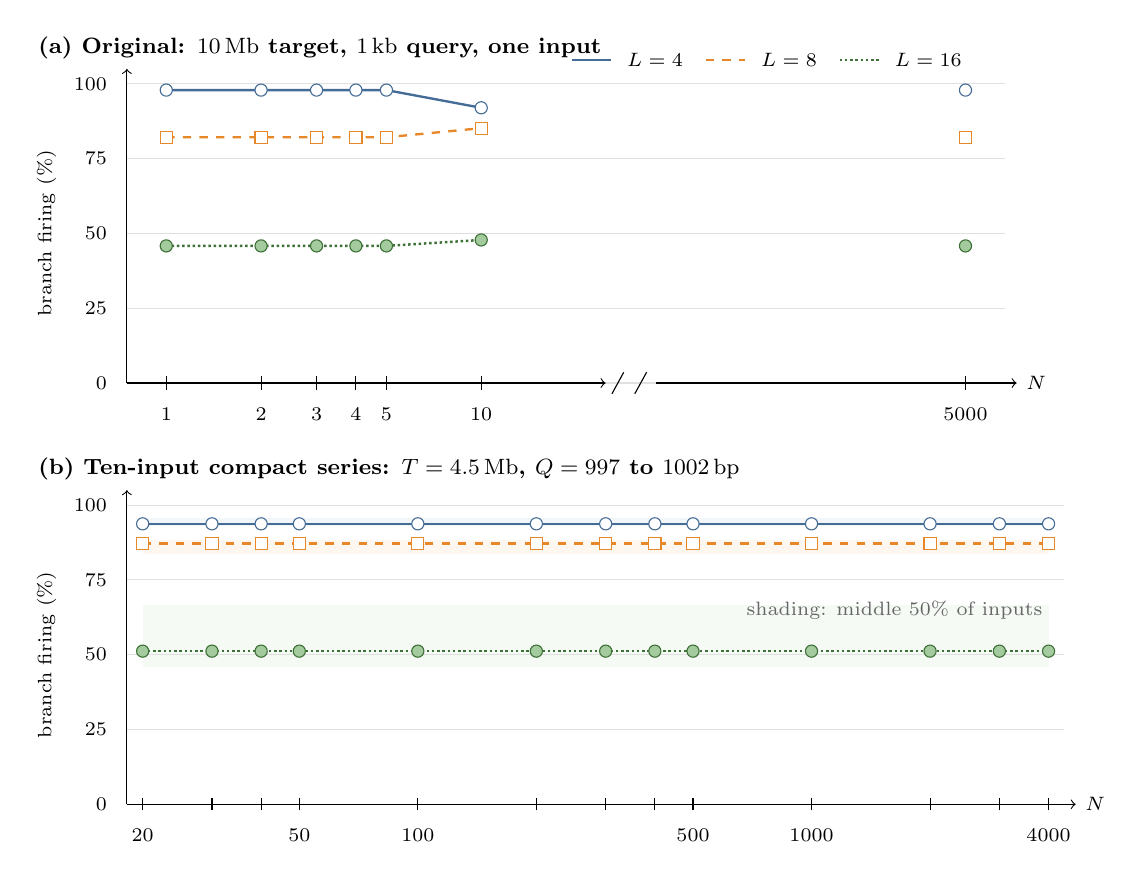
\begin{tikzpicture}[
  font=\scriptsize,
  runl four/.style={draw=chainBlue!90!black,line width=.85pt},
  runl eight/.style={
    draw=chainOrange!95!black,line width=.85pt,dashed},
  runl sixteen/.style={
    draw=chainGreen!70!black,line width=.9pt,densely dotted},
  runl mark four/.style={
    circle,draw=chainBlue!90!black,fill=white,
    minimum size=4.4pt,inner sep=0pt},
  runl mark eight/.style={
    rectangle,draw=chainOrange!95!black,fill=white,
    minimum size=4.4pt,inner sep=0pt},
  runl mark sixteen/.style={
    circle,draw=chainGreen!70!black,fill=chainGreen!55,
    minimum size=4.4pt,inner sep=0pt}
]
  % Panel (a): original 10 Mb / 1 kb occurrence sweep.
  \begin{scope}[x=1cm,y=.038cm,xshift=1.55cm,yshift=6.05cm]
    \node[anchor=west,font=\bfseries\footnotesize] at (-1.25,112)
      {(a) Original: \(10\,\mathrm{Mb}\) target,
       \(1\,\mathrm{kb}\) query, one input};

    \foreach \yy in {0,25,50,75,100} {
      \draw[black!12] (0,\yy)--(11.15,\yy);
      \node[anchor=east] at (-.13,\yy) {\yy};
    }
    \draw[->] (0,0)--(6.08,0);
    \draw[->] (6.72,0)--(11.30,0)
      node[anchor=west] {\(N\)};
    \draw[->] (0,0)--(0,105);
    \node[rotate=90] at (-1.02,50)
      {branch firing (\%)};
    \draw (6.16,-3.6)--(6.31,3.6);
    \draw (6.45,-3.6)--(6.60,3.6);

    \foreach \xx/\lab in {
      .50/1,1.7041/2,2.4085/3,2.9082/4,
      3.2959/5,4.50/10,10.65/5000} {
      \draw (\xx,-2.2)--(\xx,2.2);
      \node[anchor=north] at (\xx,-5.0) {\lab};
    }

    \draw[runl four] plot coordinates {
      (.50,97.9167) (1.7041,97.9167) (2.4085,97.9167)
      (2.9082,97.9167) (3.2959,97.9167) (4.50,92.0000)};
    \draw[runl eight] plot coordinates {
      (.50,82.1429) (1.7041,82.1429) (2.4085,82.1429)
      (2.9082,82.1429) (3.2959,82.1429) (4.50,85.1852)};
    \draw[runl sixteen] plot coordinates {
      (.50,45.8333) (1.7041,45.8333) (2.4085,45.8333)
      (2.9082,45.8333) (3.2959,45.8333) (4.50,47.8261)};

    \foreach \xx/\yy in {
      .50/97.9167,1.7041/97.9167,2.4085/97.9167,
      2.9082/97.9167,3.2959/97.9167,4.50/92.0000}
      \node[runl mark four] at (\xx,\yy) {};
    \foreach \xx/\yy in {
      .50/82.1429,1.7041/82.1429,2.4085/82.1429,
      2.9082/82.1429,3.2959/82.1429,4.50/85.1852}
      \node[runl mark eight] at (\xx,\yy) {};
    \foreach \xx/\yy in {
      .50/45.8333,1.7041/45.8333,2.4085/45.8333,
      2.9082/45.8333,3.2959/45.8333,4.50/47.8261}
      \node[runl mark sixteen] at (\xx,\yy) {};

    \node[runl mark four] at (10.65,97.9167) {};
    \node[runl mark eight] at (10.65,82.1429) {};
    \node[runl mark sixteen] at (10.65,45.8333) {};

    \draw[runl four] (5.65,108)--(6.15,108);
    \node[anchor=west] at (6.23,108) {\(L=4\)};
    \draw[runl eight] (7.35,108)--(7.85,108);
    \node[anchor=west] at (7.93,108) {\(L=8\)};
    \draw[runl sixteen] (9.05,108)--(9.55,108);
    \node[anchor=west] at (9.63,108) {\(L=16\)};
  \end{scope}

  % Panel (b): corrected ten-input compact series.
  \begin{scope}[x=1cm,y=.038cm,xshift=1.55cm,yshift=.70cm]
    \node[anchor=west,font=\bfseries\footnotesize] at (-1.25,112)
      {(b) Ten-input compact series: \(\lvert T\rvert=4.5\,\mathrm{Mb}\),
       \(\lvert Q\rvert=997\) to \(1002\,\mathrm{bp}\)};

    \path[fill=chainBlue!45,fill opacity=.15]
      (.20,93.1008) rectangle (11.7051,95.7639);
    \path[fill=chainOrange!55,fill opacity=.13]
      (.20,83.5000) rectangle (11.7051,88.3462);
    \path[fill=chainGreen!45,fill opacity=.13]
      (.20,45.9957) rectangle (11.7051,66.7293);

    \foreach \yy in {0,25,50,75,100} {
      \draw[black!12] (0,\yy)--(11.90,\yy);
      \node[anchor=east] at (-.13,\yy) {\yy};
    }
    \draw[->] (0,0)--(12.05,0)
      node[anchor=west] {\(N\)};
    \draw[->] (0,0)--(0,105);
    \node[rotate=90] at (-1.02,50)
      {branch firing (\%)};

    \foreach \xx in {
      .20,1.0805,1.7051,2.1897,3.6949,5.2000,6.0805,
      6.7051,7.1897,8.6949,10.2000,11.0805,11.7051}
      \draw (\xx,-2.0)--(\xx,2.0);
    \foreach \xx/\lab in {
      .20/20,2.1897/50,3.6949/100,
      7.1897/500,8.6949/1000,11.7051/4000}
      \node[anchor=north] at (\xx,-5.0) {\lab};

    \draw[runl four] (.20,93.7473)--(11.7051,93.7473);
    \draw[runl eight] (.20,87.2283)--(11.7051,87.2283);
    \draw[runl sixteen] (.20,51.1905)--(11.7051,51.1905);

    \foreach \xx in {
      .20,1.0805,1.7051,2.1897,3.6949,5.2000,6.0805,
      6.7051,7.1897,8.6949,10.2000,11.0805,11.7051} {
      \node[runl mark four] at (\xx,93.7473) {};
      \node[runl mark eight] at (\xx,87.2283) {};
      \node[runl mark sixteen] at (\xx,51.1905) {};
    }
    \node[anchor=east,text=black!60] at (11.75,65)
      {shading: middle 50\% of inputs};
  \end{scope}
\end{tikzpicture}
\caption{First-path branch firing on random-sequence occurrence sweeps.
The plotted value is \(100B_L/E_L\).  Horizontal positions are logarithmic in
\(N\) within each unbroken axis segment.  Panel~(a) shows every defined result
from the original sweep over \(N\) with \(k=15\) and \(w=10\).
The axis break spans the tested values between \(N=20\) and \(N=4000\), for
which no score-qualified chain end was available.  The \(N=5000\) point is
plotted separately.  Panel~(b) shows the median over ten generated inputs at
each tested \(N\).  Its bands span the middle half of those ten values.  Every
panel~(b) run had a defined first path.}
\label{fig:chaining-runl-random-occurrences}
\end{figure}

Panel~(a) records the original run.  Its missing middle prevents an estimate
of the trend over \(N\).  The ten-input compact series produced a defined value for
all 13 selected \(N\) values spanning 20 to 4000.  Its median firing rates were
93.75 percent for \(L=4\), 87.23 percent for \(L=8\), and 51.19 percent for
\(L=16\).  For each generated input, all \(N\) values used the same sequence
background.  The measured path length and branch counters stayed constant as
\(N\) changed.  The selected copy and absolute anchor-array positions could
change.  The recorded \(\operatorname{Run}_L\) outcomes produced the flat
lines.  The earlier three-input compact pilot is not plotted.

The size controls kept \(k\), \(w\), mutation probabilities, and minimap2
parameters fixed.  They tested \(N=20\) and \(N=4000\).
Figure~\ref{fig:chaining-runl-random-sizes} shows the three target/query size
pairs that produced defined percentages: approximately
\(4.5\,\mathrm{Mb}/1\,\mathrm{kb}\), \(40\,\mathrm{Mb}/4\,\mathrm{kb}\),
and \(80\,\mathrm{Mb}/8\,\mathrm{kb}\).  The
\(10\,\mathrm{Mb}/1\,\mathrm{kb}\), \(20\,\mathrm{Mb}/2\,\mathrm{kb}\),
and \(40\,\mathrm{Mb}/1\,\mathrm{kb}\) controls produced no defined
percentage at either tested \(N\).

\begin{figure}[H]
\centering
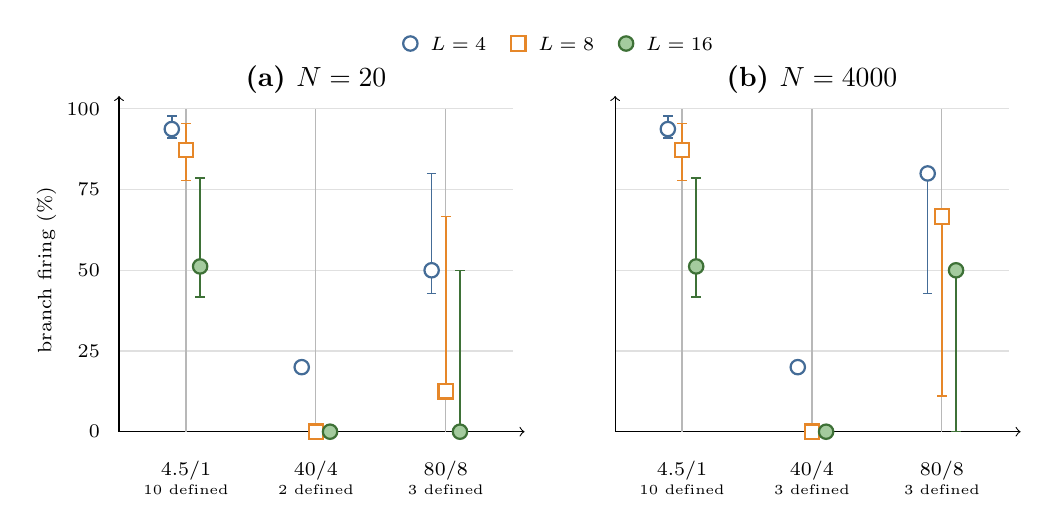
\begin{tikzpicture}[
  font=\scriptsize,
  runl mark four/.style={
    circle,draw=chainBlue!90!black,fill=white,line width=.8pt,
    minimum size=5.2pt,inner sep=0pt},
  runl mark eight/.style={
    rectangle,draw=chainOrange!95!black,fill=white,line width=.8pt,
    minimum size=5.2pt,inner sep=0pt},
  runl mark sixteen/.style={
    circle,draw=chainGreen!70!black,fill=chainGreen!55,line width=.8pt,
    minimum size=5.2pt,inner sep=0pt},
  runl whisk four/.style={draw=chainBlue!90!black,line width=.55pt},
  runl whisk eight/.style={draw=chainOrange!95!black,line width=.55pt},
  runl whisk sixteen/.style={draw=chainGreen!70!black,line width=.55pt}
]
  \node[runl mark four] at (5.05,5.55) {};
  \node[anchor=west] at (5.18,5.55) {\(L=4\)};
  \node[runl mark eight] at (6.42,5.55) {};
  \node[anchor=west] at (6.55,5.55) {\(L=8\)};
  \node[runl mark sixteen] at (7.79,5.55) {};
  \node[anchor=west] at (7.92,5.55) {\(L=16\)};

  \begin{scope}[x=1cm,y=.041cm,xshift=1.35cm,yshift=.62cm]
    \node[font=\bfseries] at (2.50,109) {(a) \(N=20\)};
    \foreach \yy in {0,25,50,75,100} {
      \draw[black!12] (0,\yy)--(5.00,\yy);
      \node[anchor=east] at (-.12,\yy) {\yy};
    }
    \draw[->] (0,0)--(5.15,0);
    \draw[->] (0,0)--(0,104);
    \node[rotate=90] at (-.92,50) {branch firing (\%)};

    \foreach \xx in {.85,2.50,4.15}
      \draw[black!28] (\xx,0)--(\xx,100);
    \foreach \xx/\lo/\hi in {
      .67/90.9091/97.7273,3.97/42.8571/80.0000} {
      \draw[runl whisk four] (\xx,\lo)--(\xx,\hi);
      \draw[runl whisk four] (\xx-.06,\lo)--(\xx+.06,\lo);
      \draw[runl whisk four] (\xx-.06,\hi)--(\xx+.06,\hi);
    }
    \foreach \xx/\lo/\hi in {
      .85/77.7778/95.4545,4.15/11.1111/66.6667} {
      \draw[runl whisk eight] (\xx,\lo)--(\xx,\hi);
      \draw[runl whisk eight] (\xx-.06,\lo)--(\xx+.06,\lo);
      \draw[runl whisk eight] (\xx-.06,\hi)--(\xx+.06,\hi);
    }
    \foreach \xx/\lo/\hi in {
      1.03/41.6667/78.5714,4.33/0.0000/50.0000} {
      \draw[runl whisk sixteen] (\xx,\lo)--(\xx,\hi);
      \draw[runl whisk sixteen] (\xx-.06,\lo)--(\xx+.06,\lo);
      \draw[runl whisk sixteen] (\xx-.06,\hi)--(\xx+.06,\hi);
    }
    \node[runl mark four] at (.67,93.7473) {};
    \node[runl mark eight] at (.85,87.2283) {};
    \node[runl mark sixteen] at (1.03,51.1905) {};
    \node[runl mark four] at (2.32,20.0000) {};
    \node[runl mark eight] at (2.50,0.0000) {};
    \node[runl mark sixteen] at (2.68,0.0000) {};
    \node[runl mark four] at (3.97,50.0000) {};
    \node[runl mark eight] at (4.15,12.5000) {};
    \node[runl mark sixteen] at (4.33,0.0000) {};

    \node[anchor=north,align=center] at (.85,-6)
      {4.5/1\\[-1pt]\tiny 10 defined};
    \node[anchor=north,align=center] at (2.50,-6)
      {40/4\\[-1pt]\tiny 2 defined};
    \node[anchor=north,align=center] at (4.15,-6)
      {80/8\\[-1pt]\tiny 3 defined};
  \end{scope}

  \begin{scope}[x=1cm,y=.041cm,xshift=7.65cm,yshift=.62cm]
    \node[font=\bfseries] at (2.50,109) {(b) \(N=4000\)};
    \foreach \yy in {0,25,50,75,100}
      \draw[black!12] (0,\yy)--(5.00,\yy);
    \draw[->] (0,0)--(5.15,0);
    \draw[->] (0,0)--(0,104);

    \foreach \xx in {.85,2.50,4.15}
      \draw[black!28] (\xx,0)--(\xx,100);
    \foreach \xx/\lo/\hi in {
      .67/90.9091/97.7273,3.97/42.8571/80.0000} {
      \draw[runl whisk four] (\xx,\lo)--(\xx,\hi);
      \draw[runl whisk four] (\xx-.06,\lo)--(\xx+.06,\lo);
      \draw[runl whisk four] (\xx-.06,\hi)--(\xx+.06,\hi);
    }
    \foreach \xx/\lo/\hi in {
      .85/77.7778/95.4545,4.15/11.1111/66.6667} {
      \draw[runl whisk eight] (\xx,\lo)--(\xx,\hi);
      \draw[runl whisk eight] (\xx-.06,\lo)--(\xx+.06,\lo);
      \draw[runl whisk eight] (\xx-.06,\hi)--(\xx+.06,\hi);
    }
    \foreach \xx/\lo/\hi in {
      1.03/41.6667/78.5714,4.33/0.0000/50.0000} {
      \draw[runl whisk sixteen] (\xx,\lo)--(\xx,\hi);
      \draw[runl whisk sixteen] (\xx-.06,\lo)--(\xx+.06,\lo);
      \draw[runl whisk sixteen] (\xx-.06,\hi)--(\xx+.06,\hi);
    }
    \node[runl mark four] at (.67,93.7473) {};
    \node[runl mark eight] at (.85,87.2283) {};
    \node[runl mark sixteen] at (1.03,51.1905) {};
    \node[runl mark four] at (2.32,20.0000) {};
    \node[runl mark eight] at (2.50,0.0000) {};
    \node[runl mark sixteen] at (2.68,0.0000) {};
    \node[runl mark four] at (3.97,80.0000) {};
    \node[runl mark eight] at (4.15,66.6667) {};
    \node[runl mark sixteen] at (4.33,50.0000) {};

    \node[anchor=north,align=center] at (.85,-6)
      {4.5/1\\[-1pt]\tiny 10 defined};
    \node[anchor=north,align=center] at (2.50,-6)
      {40/4\\[-1pt]\tiny 3 defined};
    \node[anchor=north,align=center] at (4.15,-6)
      {80/8\\[-1pt]\tiny 3 defined};
  \end{scope}

\end{tikzpicture}
\caption{Median first-path branch firing for random-sequence size controls
with a defined path.  Each point is the median of the defined per-input
percentages.  The number of contributing inputs is printed below it.  The
horizontal labels give target length in megabases followed by query length in
kilobases.  Query lengths were 997 to 1002 bases, 3998 to 4004 bases, and 7999
to 8008 bases.  Vertical whiskers span the smallest and largest per-input
percentages.  Within each size pair, markers and whiskers are offset
horizontally only for visibility.  A plotted zero
means that a measured path existed and \(B_L=0\).  Runs with no score-qualified
chain end are omitted.  At \(40\,\mathrm{Mb}/4\,\mathrm{kb}\) and \(N=20\),
one of three generated inputs had no defined percentage, so the median uses
the other two.  The omitted target/query size pairs are
\(10\,\mathrm{Mb}/1\,\mathrm{kb}\), \(20\,\mathrm{Mb}/2\,\mathrm{kb}\),
and \(40\,\mathrm{Mb}/1\,\mathrm{kb}\) at both tested \(N\) values.}
\label{fig:chaining-runl-random-sizes}
\end{figure}

In the 40-Mb/4-kb and 80-Mb/8-kb controls, default occurrence filtering left
short first paths.  Query-side filtering removed none of their generated
minimizers.  For both sizes, the adaptive reference cutoff
\texttt{mid\_occ} remained 10.  Most repeated source minimizers had
approximately \(N\) reference occurrences.  A few also matched elsewhere in
the random target.  These counts exceeded \texttt{mid\_occ}.  Reference
occurrence filtering removed between 98.79 and 98.90 percent of the raw anchor
hits.  For each consecutive group above the cutoff, \texttt{occ\_dist}=500
set the number of minimizers that could remain from its query-coordinate
span.  It kept those with the smallest reference occurrence counts.  Every
defined 4-kb input had \(q=8\), while the 8-kb inputs had
\(q\in\{15,16,17\}\).  The longer query produced a larger limit under this
rule.  Target length also affects the adaptive cutoff, so this comparison does
not isolate query length.

The 4.5-Mb/1-kb series used larger adaptive cutoffs.  They were 21 for
\(N=20\) and 4001 for \(N=4000\).  Reference occurrence filtering retained
every anchor hit.  On each validated first path, every predecessor index was
one less than the current index.  These paths contained 163 to 187 anchors and
gave the higher firing percentages shown in
Figure~\ref{fig:chaining-runl-random-sizes}.

After filtering, \(\operatorname{Run}_L\) is evaluated from the predecessor
indices on these short paths.  All recorded bounds tests passed.  A displayed
zero therefore means that the predecessor-index equalities in
\(\operatorname{Run}_L\) failed at every loop evaluation.  The observed
first-path profiles were
\[
\begin{array}{c|ccc}
q & \operatorname{Fire}_4 & \operatorname{Fire}_8 &
    \operatorname{Fire}_{16} \\
\hline
8  & 1/5=20\% & 0/8=0\%     & 0/8=0\% \\
15 & 3/6=50\% & 1/8=12.5\%  & 0/15=0\% \\
16 & 3/7=42.86\% & 1/9=11.11\% & 0/16=0\% \\
17 & 4/5=80\% & 2/3=66.67\% & 1/2=50\%
\end{array}
\]
Every defined 40-Mb/4-kb input had the first profile.  It provided one
four-wide batch and no eight-wide or sixteen-wide batch.  For the 80-Mb/8-kb
controls, the path lengths at \(N=20\) were 16, 15, and 17.  At \(N=4000\)
they were 16, 17, and 17.  A 17-anchor path was the only observed profile with
one sixteen-wide batch.  That batch was followed by one scalar evaluation, so
\(B_{16}=1\), \(E_{16}=2\), and the firing percentage was 50 percent.  The
other profiles gave zero.  These discrete outcomes produce the whisker from
0 to 50 percent in Figure~\ref{fig:chaining-runl-random-sizes}.

The 40-Mb and 80-Mb conditions contained only two or three inputs with a
defined percentage.  Their whiskers are descriptive ranges.  The results do
not establish a length trend.  Minimap2 required a chaining score of at least
40.  The omitted 40-Mb/4-kb input at \(N=20\) had no anchor reaching that
threshold.

These measurements describe opportunities for the first-path vector branch.
They do not measure BioseqDB execution time.  The cost of failed checks and
the speed of successful vector batches must be evaluated by a BioseqDB
runtime benchmark.  Initial dynamic-programming and later RMQ calls were
recorded separately.  Table~\ref{tab:chaining-runl-firing} and
Figures~\ref{fig:chaining-runl-random-occurrences}
and~\ref{fig:chaining-runl-random-sizes} report only the initial
dynamic-programming call used by the special first-path loop.

\subsection{BioseqDB SIMD performance comparison}


This test configuration used a
\(500{,}000{,}000\)-base reference and one query fragment whose configured mean
length is \(5{,}000{,}000\) bases (with two samples).

\begin{figure}[H]
\centering
\begin{tikzpicture}[scale=1.0,transform shape,x=1cm,y=1cm,
  font=\footnotesize,>=Latex]
  \node[anchor=west,font=\bfseries] at (.10,9.55)
    {(a) Chaining};
  \draw[->] (2.50,5.10)--(12.15,5.10) node[right] {ms};
  \foreach \x/\lab in {0/0,20/20,40/40,60/60,80/80,100/100,120/120}
    {
      \draw (2.50+.075*\x,5.00)--(2.50+.075*\x,5.20);
      \node[anchor=north] at (2.50+.075*\x,4.97) {\lab};
    }
  \node[anchor=east] at (2.35,8.55) {B1 scalar};
  \node[anchor=east] at (2.35,7.35) {B1 exact SIMD};
  \node[anchor=east] at (2.35,6.15) {B5 bounded SIMD};
  \draw[fill=chainGray!32,draw=chainGray!90!black]
    (2.50,8.17) rectangle (2.50+.075*115.286,8.93);
  \draw[fill=chainBlue!22,draw=chainBlue!90!black]
    (2.50,6.97) rectangle (2.50+.075*101.885,7.73);
  \draw[fill=chainOrange!25,draw=chainOrange!95!black]
    (2.50,5.77) rectangle (2.50+.075*67.012,6.53);
  \node[anchor=west] at (2.66+.075*115.286,8.55) {115.286};
  \node[anchor=west] at (2.66+.075*101.885,7.35) {101.885};
  \node[anchor=west] at (2.66+.075*67.012,6.15) {67.012};

  \node[anchor=west,font=\bfseries] at (.10,4.15)
    {(b) Backtrack};
  \draw[->] (2.50,-.30)--(10.10,-.30) node[right] {ms};
  \foreach \x/\lab in {0/0,2/2,4/4,6/6,8/8,10/10,12/12}
    {
      \draw (2.50+.58*\x,-.40)--(2.50+.58*\x,-.20);
      \node[anchor=north] at (2.50+.58*\x,-.43) {\lab};
    }
  \node[anchor=east] at (2.35,3.15) {B1 scalar};
  \node[anchor=east] at (2.35,1.95) {B1 exact SIMD};
  \node[anchor=east] at (2.35,.75) {B5 bounded SIMD};
  \draw[fill=chainGray!32,draw=chainGray!90!black]
    (2.50,2.77) rectangle (2.50+.58*11.769,3.53);
  \draw[fill=chainBlue!22,draw=chainBlue!90!black]
    (2.50,1.57) rectangle (2.50+.58*8.549,2.33);
  \draw[fill=chainOrange!25,draw=chainOrange!95!black]
    (2.50,.37) rectangle (2.50+.58*8.345,1.13);
  \node[anchor=west] at (2.65+.58*11.769,3.15) {11.769};
  \node[anchor=west] at (2.65+.58*8.549,1.95) {8.549};
  \node[anchor=west] at (2.65+.58*8.345,.75) {8.345};
\end{tikzpicture}
\caption{Recorded times for the three CPU modes}
\label{fig:chaining-mode-times}
\end{figure}

The figure above depicts only two runs and presents only quick prototyping test measurements to judge if we are going in right direction.

%%%%%% EDIT BELOW HERE
\section{Range minimum query chaining}
\label{sec:chaining-rmq-idea}

The ordered predecessor scan in B1 can calculate many complete link scores for
one target.  The B4 algorithm first compares a value that depends only on the
earlier anchor:
\begin{equation}
  h(j)=f_j+\frac{\lambda_g}{2}(r_j+q_j).
\label{eq:chaining-rmq-h}
\end{equation}
Once \(f_j\) is known, the same \(h(j)\) can be reused for every later target.
An RMQ tree stores
\(\pi(j)=-h(j)\).  A query for the smallest priority therefore returns an
anchor with the largest \(h(j)\) inside a query-coordinate interval.

This is a candidate-selection method.  The tree does not store the complete
target-dependent value \(f_j+E(j,i)\).  Minimap2 calculates that value after
the query.  It can also scan a narrower local interval when the selected link
is not an exact extension.  This design is used by minimap2's RMQ chaining
mode and by assembly presets that need to consider links across long gaps.
In this section, \(f_j+E(j,i)\) is the complete proposed chain score,
abbreviated to complete score.

\subsection{Minimap2 RMQ}
\label{sec:chaining-minimap2-rmq}

Let
\[
  D=\max\{\texttt{max\_dist},\texttt{bw}\}.
\]
The optional local scan uses
\[
  D_{\mathrm{in}}
  =\min\{\max\{\texttt{max\_dist\_inner},0\},D\}.
\]
Minimap2 maintains an active set of earlier anchors on the same reference and
strand as the current target \(i\).  It removes anchors when
\(r_i-r_j>D\), when the reference or strand changes, or when the configured
tree-size cap is exceeded.  Anchors at the current reference coordinate are
held outside the tree until the scan moves to a larger coordinate.  Every
stored candidate therefore has \(r_j<r_i\).

The AVL search key and stored priority are
\[
  K_j=(q_j,j),
  \qquad
  \pi(j)=-h(j).
\]
The index \(j\) keeps equal query coordinates as separate nodes.  Each node
also caches the anchor with the smallest priority in its subtree.  The query uses the closed
interval between
\begin{equation}
  K_i^{\mathrm{lo}}=(q_i-D,\mathrm{INT32\_MAX}),
  \qquad
  K_i^{\mathrm{hi}}=(q_i,0).
\label{eq:chaining-rmq-key-range}
\end{equation}
For ordinary positive indices, these composite keys admit
\(q_i-D<q_j<q_i\).  Figure~\ref{fig:chaining-minimap2-rmq} shows the complete
selection.
The tree query does not define a stable index tie rule when two anchors have
the same \(h(j)\).

\begin{figure}[H]
\centering
\begin{tikzpicture}[x=1cm,y=1cm,font=\scriptsize,>=Latex]
  \node[anchor=west,font=\bfseries] at (.05,6.35)
    {(a) Maintain the active set};
  \node[anchor=west,font=\bfseries] at (4.85,6.35)
    {(b) Query cached values};
  \node[anchor=west,font=\bfseries] at (10.05,6.35)
    {(c) Check the selected link};

  % Active reference window.
  \draw[fill=chainGray!10,draw=chainGray!80!black]
    (.15,4.85) rectangle (1.00,5.55);
  \node at (.575,5.20) {\(j_0\)};
  \draw[very thick,draw=chainOrange!95!black]
    (.10,4.78)--(1.05,5.62);
  \node[anchor=north,text=chainGray!90!black] at (.575,4.72) {expired};

  \foreach \x/\lab in {1.25/\(j_1\),2.20/\(j_2\)}
    {
      \draw[fill=chainBlue!13,draw=chainBlue!90!black]
        (\x,4.85) rectangle (\x+.85,5.55);
      \node at (\x+.425,5.20) {\lab};
    }
  \draw[fill=chainGreen!14,draw=chainGreen!80!black,very thick]
    (4.05,4.85) rectangle (4.70,5.55);
  \node at (4.375,5.20) {\(i\)};
  \draw[fill=chainOrange!14,draw=chainOrange!95!black,dashed]
    (4.05,3.75) rectangle (4.70,4.45);
  \node at (4.375,4.10) {\(j_3\)};
  \draw[dashed,draw=chainOrange!95!black]
    (4.375,4.45)--(4.375,4.85);
  \node[align=center,text=chainOrange!95!black,anchor=north]
    at (4.375,3.68) {same \(r\) as \(i\)\\insert later};
  \draw[<->,draw=chainBlue!90!black,thick]
    (1.25,5.82)--(4.70,5.82);
  \node[anchor=south,text=chainBlue!90!black] at (2.98,5.84)
    {reference distance at most \(D\)};

  % Query-coordinate strip and AVL tree.
  \foreach \x/\q/\fillc in {
      4.95/7/chainGray!10,
      5.75/11/chainBlue!12,
      6.55/14/chainOrange!22,
      7.35/18/chainBlue!12,
      8.15/22/chainBlue!12,
      8.95/27/chainGreen!14}
    {
      \draw[fill=\fillc,draw=black!55]
        (\x,5.08) rectangle (\x+.62,5.62);
      \node at (\x+.31,5.35) {\q};
    }
  \draw[<->,draw=chainOrange!95!black,thick]
    (5.65,4.77)--(8.85,4.77);
  \node[anchor=north] at (7.56,4.68)
    {\(q_i-D<q_j<q_i\)};

  \node[draw=chainBlue!90!black,fill=chainBlue!10,
    minimum width=1.22cm,minimum height=.74cm,align=center]
    (r17) at (7.25,3.70) {\(q=18\)\\max \(h=44\)};
  \node[draw=chainBlue!90!black,fill=chainBlue!10,
    minimum width=1.22cm,minimum height=.74cm,align=center]
    (r11) at (5.75,2.55) {\(q=11\)\\max \(h=44\)};
  \node[draw=chainBlue!90!black,fill=chainBlue!10,
    minimum width=1.22cm,minimum height=.74cm,align=center]
    (r22) at (8.75,2.55) {\(q=22\)\\max \(h=29\)};
  \node[draw=chainOrange!95!black,fill=chainOrange!22,very thick,
    minimum width=1.22cm,minimum height=.70cm,align=center]
    (r14) at (6.35,1.35) {\(q=14\)\\\(h=44\)};
  \node[draw=chainGray!80!black,fill=chainGray!10,
    minimum width=1.22cm,minimum height=.70cm,align=center]
    (r7) at (5.10,1.35) {\(q=7\)\\\(h=20\)};
  \draw[thick] (r17)--(r11);
  \draw[thick] (r17)--(r22);
  \draw[thick] (r11)--(r7);
  \draw[thick] (r11)--(r14);

  % Complete-score path.
  \draw[fill=chainOrange!18,draw=chainOrange!95!black]
    (10.15,4.85) rectangle (11.72,5.55);
  \node[align=center] at (10.935,5.20) {selected\\\(j^\star\)};
  \draw[chain flow] (11.72,5.20)--(12.18,5.20);
  \draw[fill=chainBlue!12,draw=chainBlue!90!black]
    (12.18,4.75) rectangle (14.15,5.65);
  \node[align=center] at (13.165,5.20)
    {\(f_{j^\star}+E(j^\star,i)\)};

  \draw[chain flow] (13.165,4.75)--(13.165,3.95);
  \draw[fill=chainGreen!13,draw=chainGreen!80!black]
    (11.95,3.05) rectangle (14.38,3.95);
  \node[align=center] at (13.165,3.50)
    {bandwidth and\\strict score check};

  \draw[chain flow] (13.165,3.05)--(13.165,2.25);
  \draw[fill=chainGreen!13,draw=chainGreen!80!black]
    (12.15,1.45) rectangle (14.18,2.25);
  \node at (13.165,1.85) {store \(f_i,p_i\)};

  \draw[dashed,draw=chainOrange!95!black,-{Latex[length=1.7mm]}]
    (12.18,4.95)--(11.68,4.95)--(11.68,2.20)--(11.85,2.20);
  \node[align=left,anchor=east,text=chainOrange!95!black]
    at (11.72,1.55) {narrow local scan\\if link is not exact};
\end{tikzpicture}
\caption{Minimap2 RMQ for one target.  Anchors outside the reference window
are removed, and anchors at the target's reference coordinate are not yet
inserted.  The augmented AVL query selects one \(j^\star\) using \(h(j)\).
Minimap2 then calculates the complete link score for \(j^\star\).  The dashed path is the
optional local scan.}
\label{fig:chaining-minimap2-rmq}
\label{fig:chaining-rmq-contrast}
\end{figure}

Algorithm~\ref{alg:chaining-minimap2-rmq} states the forward calculation.  The
maintenance calls insert a completed reference-coordinate group and remove
entries that fail the active-set rules above.  Each maintenance helper owns
an independent scan cursor, reads the anchor array and completed scores, and
updates the named tree.  \textsc{RangeBest} returns the anchor with the largest
\(h(j)\) in the composite-key interval.

\begin{algorithm}[H]
\caption{Minimap2 RMQ forward chaining}
\label{alg:chaining-minimap2-rmq}
\footnotesize
\begin{algorithmic}[1]
  \Require sorted anchors \(a_0,\ldots,a_{n-1}\), distance \(D\),
    inner distance \(D_{\mathrm{in}}\), bandwidth \(B\), tree cap \(C\),
    skip limit \(S\)
  \Ensure scores \(f\) and absolute predecessor indices \(p\)
  \Function{Minimap2RMQForward}{\(a,D,D_{\mathrm{in}},B,C,S\)}
    \State \(T\gets\varnothing,\quad T_{\mathrm{in}}\gets\varnothing\)
          \Comment{augmented AVL trees}
    \State \(t\gets(0,\ldots,0)\)
          \Comment{B1 marks for the optional local scan}
    \For{\(i\gets0\) \textbf{to} \(n-1\)}
      \State \Call{InsertCompletedReferenceGroup}{\(T,a,f,i\)}
      \If{\(D_{\mathrm{in}}>0\)}
        \State \Call{InsertCompletedReferenceGroup}{\(T_{\mathrm{in}},a,f,i\)}
      \EndIf
      \State \Call{RemoveExpiredEntries}{\(T,a,i,D,C\)}
      \If{\(D_{\mathrm{in}}>0\)}
        \State \Call{RemoveExpiredEntries}{\(T_{\mathrm{in}},a,i,D_{\mathrm{in}},C\)}
      \EndIf
      \State \(f_i\gets\ell_i,\quad p_i\gets-1\)
      \State \(j^\star\gets
        \Call{RangeBest}{T,(q_i-D,\mathrm{INT32\_MAX}),(q_i,0)}\)
      \If{\(j^\star\neq\bot\)}
        \State \((e,\delta,\mathrm{exact})\gets
          \Call{CompleteLink}{j^\star,i}\)
              \Comment{\(e=E(j^\star,i)\)}
        \If{\(\delta\leq B\land f_{j^\star}+e>f_i\)}
          \State \(f_i\gets f_{j^\star}+e,\quad p_i\gets j^\star\)
        \EndIf
        \If{\(\neg\mathrm{exact}\land T_{\mathrm{in}}\neq\varnothing
             \land q_i>0\)}
          \State \((f_i,p_i)\gets
            \Call{ScanLocalInterval}{T_{\mathrm{in}},i,D_{\mathrm{in}},B,S,f,p,t}\)
              \Comment{complete scores with the B1 mark and skip rule}
        \EndIf
      \EndIf
    \EndFor
    \State \Return \(f,p\)
  \EndFunction
\end{algorithmic}
\end{algorithm}

An exact extension has
\[
  \delta(j^\star,i)=0
  \quad\land\quad
  g(j^\star,i)\leq\ell_{j^\star}.
\]
If the selected link is not exact and the inner tree is enabled, the local
scan visits retained anchors with
\[
  q_i-D_{\mathrm{in}}\leq q_j\leq q_i-1
\]
from larger to smaller query coordinate.  It calculates the complete score
for every visited candidate.  The bandwidth check and the B1 mark and skip
rule apply inside this scan.  The primary tree is not queried for a second
choice.

Tree insertion, deletion, and the primary query cost
\(O(\log M_{\max})\) per anchor, where \(M_{\max}\) is the largest active
tree.  If target \(i\) visits \(k_i\) local candidates, the forward cost is
\[
  O(n\log M_{\max})+
  O\!\left(\sum_i k_i\right).
\]
The local scans can still make this quadratic.  The parameter
\texttt{max\_chain\_iter} is not used.  The parameter
\texttt{max\_chain\_skip} affects only the local scan.

Minimap2 selects B1 or RMQ for the first chaining call according to the RMQ
flag.  A
later long-gap joining condition can sort the retained anchors and call RMQ
again with a wider bandwidth.  This later call is conditional.  It can follow
either an initial B1 call or an initial RMQ call.
\leavevmode\coderef{minimap2/lchain.c}
  {Minimap2 RMQ forward pass}{mg_lchain_rmq}{250}
\leavevmode\coderef{minimap2/krmq.h}
  {Augmented AVL interval query}{__KRMQ_RMQ}{110}
\leavevmode\coderef{minimap2/map.c}
  {RMQ selection and wider joining}{mm_map_frag_core}{275}

\subsection{BioseqDB RMQ differences}
\label{sec:chaining-bioseqdb-rmq-summary}

BioseqDB reuses the high-level procedure in
Algorithm~\ref{alg:chaining-minimap2-rmq}, including the augmented AVL tree
and the preliminary value \(h(j)\).  Its RMQ configuration sets the local
distance to zero, so only the primary tree is used.  The following differences
affect the selected predecessor:

\begin{itemize}
  \item BioseqDB stores full-width reference and query coordinates.  It
    searches the inclusive
    composite-key interval
    \[
      (q_i-D,\mathrm{INT64\_MIN})
      \ \ldots\
      (q_i,\mathrm{INT64\_MAX}).
    \]
    It can therefore include both query-coordinate boundaries.
  \item It calculates the selected link's diagonal width but does not reject
    the link when the width exceeds the configured bandwidth.
  \item It performs one RMQ pass.  The BioseqDB RMQ route has no local scan
    and no optional wider second call.  Neither \texttt{max\_chain\_skip} nor
    \texttt{max\_chain\_iter} affects this forward route.
  \item It uses BioseqDB's shared scalar chain extraction after the forward
    pass.  That extractor does not use minimap2's maximum-drop cut search.
\end{itemize}

Within each equal-reference group, BioseqDB orders anchors by a packed query
key.  This key contains the query-segment identifier, anchor flags, query
span, and the low 32 bits of the query position.  The full 64-bit query
position breaks a tie between equal packed keys.  Minimap2's radix pass sorts
only the packed reference key.  Equal-priority cache handling also differs,
so equal \(h(j)\) values can select different predecessor anchors.  The whole
BioseqDB RMQ route has \(O(n\log n)\) worst-case time.
Section~\ref{sec:chaining-bioseqdb} describes how this route is selected.

\section{G3SA GPU chaining}
\label{sec:chaining-b2}

G3SA moves forward scoring and backtracking to CUDA
\cite{g3sa_paper}.  Its released code is easiest to follow as four logical
phases.  These phases are not four individual CUDA launches.  Range
construction, sorting, copying, and output preparation use supporting
kernels.

\begin{enumerate}
  \item \textbf{First forward-scoring pass.}  A small range uses the short score
    kernel.  A larger range uses the tiled score kernel.
  \item \textbf{First backtracking and packing.}  G3SA applies minimap2's
    cut and marking rule, reverses accepted paths, and packs their anchors.
  \item \textbf{Conditional ranking pass.}  The retained anchors of selected
    reads are sorted again.  A short or tiled
    kernel compares \(h(j)\) and calculates one complete link score for each
    target that saved a predecessor.
  \item \textbf{Final backtracking.}  The same recovery workflow processes
    the second-pass scores and creates the final chain records.
\end{enumerate}

\info{G3SA AVL code}{The repository contains CUDA AVL support code and a
commented experimental entry point.  The active chaining pipeline does not
call that entry point.  Its second pass uses array-based short and tiled
kernels.}

Figure~\ref{fig:chaining-pipelines} defines the second-pass decision before the
individual kernels are described.  Let \(n_u\) be the number of paths retained
by the first backtracking, let \(Q\) be the query length, and let
\[
  R=q_{\mathrm{last}}-q_{\mathrm{first}}
\]
be the query-coordinate span of the first path after paths have been ordered
by their first anchor's packed target key.  This key contains the reference
identifier, strand, and reference position.  G3SA performs second-pass work for the
read when
\begin{equation}
  n_u>1
  \quad\land\quad
  \bigl(Q-R>1000\ \lor\ R>0.10Q\bigr).
\label{eq:chaining-g3sa-second-condition}
\end{equation}
The wrapper is launched for the whole batch.  Reads that fail this condition
are given an empty second-pass range.

\begin{figure}[H]
\centering
\begin{tikzpicture}[x=1cm,y=1cm,font=\footnotesize,>=Latex]
  \draw[chain muted] (.10,3.25) rectangle (1.55,4.15);
  \node at (.825,3.70) {anchors};

  \draw[chain blue] (2.10,2.92) rectangle (4.65,4.48);
  \node[font=\bfseries] at (3.375,4.15)
    {first-pass score};
  \draw[fill=chainBlue!6,draw=chainBlue!70!black]
    (2.30,3.08) rectangle (3.28,3.72);
  \node at (2.79,3.40) {short};
  \draw[fill=chainBlue!6,draw=chainBlue!70!black]
    (3.47,3.08) rectangle (4.45,3.72);
  \node at (3.96,3.40) {tiled};

  \draw[chain green] (5.20,3.15) rectangle (7.55,4.25);
  \node[align=center] at (6.375,3.70)
    {backtrack\\and pack};

  \draw[chain orange] (8.10,3.05) rectangle (10.72,4.35);
  \node[align=center] at (9.41,3.70)
    {Equation~\ref{eq:chaining-g3sa-second-condition}\\is true?};

  \draw[chain green] (11.35,3.15) rectangle (14.15,4.25);
  \node[align=center] at (12.75,3.70)
    {no: keep first-pass\\chain records};

  \draw[chain blue] (8.10,.75) rectangle (10.72,1.95);
  \node[align=center] at (9.41,1.35)
    {pool and sort\\rank again};

  \draw[chain green] (11.35,.75) rectangle (14.15,1.95);
  \node[align=center] at (12.75,1.35)
    {same backtracking\\final records};

  \draw[chain flow] (1.55,3.70)--(2.10,3.70);
  \draw[chain flow] (4.65,3.70)--(5.20,3.70);
  \draw[chain flow] (7.55,3.70)--(8.10,3.70);
  \draw[chain flow] (10.72,3.70)--(11.35,3.70)
    node[midway,above] {no};
  \draw[chain flow] (9.41,3.05)--(9.41,1.95)
    node[midway,right] {yes};
  \draw[chain flow] (10.72,1.35)--(11.35,1.35);
\end{tikzpicture}
\caption{The four logical phases of G3SA chaining.  The first score pass
chooses one of two kernel functions.  The first backtracking packs only
retained anchors.  Equation~\ref{eq:chaining-g3sa-second-condition} decides
whether those anchors enter the ranking pass and a second recovery.}
\label{fig:chaining-pipelines}
\end{figure}

\leavevmode\coderef{g3sa/minimap2/src/kernel_wrapper.cu}
  {G3SA chaining pipeline}{chaining_kernel_wrapper}{775}
\leavevmode\coderef{g3sa/minimap2/src/krmq_cuda.cu}
  {Commented CUDA AVL entry point}{gpu_chain_rmq}{406}

\subsection{Short first-pass kernel}
\label{sec:chaining-work-split}

For one inclusive anchor range with first index \(s\) and last index \(e\),
G3SA classifies the anchor-index span
\[
  d=e-s.
\]
The short kernel handles \(d\leq512\), which is at most \(513\) anchors.
The tiled kernel handles larger values.  Its two launch configurations are
described below.

The first forward-scoring pass sets \(f_i=15\) and stores no predecessor.  When a
predecessor is selected, G3SA stores its positive index distance
\[
  \widehat p_i=i-j.
\]
Backtracking therefore moves from \(i\) to \(i-\widehat p_i\).
For two anchors in the same query segment, the active first-pass parameters
use bandwidth zero, fixed span \(15\), maximum coordinate distance \(5000\),
and \(\lambda_s=0\).  Every stored same-query-segment link satisfies
\[
  0<i-j\leq5000,
  \qquad
  0<d_r(j,i)=d_q(j,i)\leq5000.
\]
Its link score reduces to
\[
  E(j,i)=\min\{15,d_r(j,i)\}.
\]
The code has a separate scoring branch for links between query segments.  The
single-query-segment case is used below because it makes the work assignment
clear.

In minimap2 B1, one target \(i\) reads earlier candidates.  The G3SA short
kernel fixes one completed source \(j\), assigns later targets to threads, and
waits before advancing to \(j+1\).  Figure~\ref{fig:chaining-work-split}
compares these directions.

\begin{figure}[H]
\centering
\begin{tikzpicture}[x=1cm,y=1cm,font=\footnotesize,>=Latex]
  \node[anchor=west,font=\bfseries] at (.15,6.75)
    {(a) minimap2 B1: fix target \(i\)};
  \node[anchor=west,font=\bfseries] at (7.35,6.75)
    {(b) G3SA short: fix source \(j\)};

  \foreach \r/\c in {
      0/1,0/2,0/3,0/4,0/5,
      1/2,1/3,1/4,1/5,
      2/3,2/4,2/5,
      3/4,3/5,
      4/5}
    \draw[fill=chainGray!12,draw=chainGray!80!black]
      (1.35+.62*\c-.27,5.72-.62*\r-.27)
      rectangle
      (1.35+.62*\c+.27,5.72-.62*\r+.27);
  \foreach \r in {0,...,4}
    \draw[fill=chainBlue!20,draw=chainBlue!90!black,very thick]
      (1.35+.62*5-.27,5.72-.62*\r-.27)
      rectangle
      (1.35+.62*5+.27,5.72-.62*\r+.27);
  \draw[fill=chainOrange!24,draw=chainOrange!95!black,very thick]
    (1.35+.62*5-.27,5.72-.62*5-.27)
    rectangle
    (1.35+.62*5+.27,5.72-.62*5+.27);
  \node at (1.35+.62*5,5.72-.62*5) {\(i\)};
  \foreach \c in {0,...,5}
    \node[anchor=south] at (1.35+.62*\c,6.06) {\scriptsize \(i_{\c}\)};
  \foreach \r in {0,...,5}
    \node[anchor=east] at (1.00,5.72-.62*\r) {\scriptsize \(j_{\r}\)};
  \draw[chain flow,draw=chainBlue!90!black]
    (5.28,2.78)--(5.28,5.40);
  \node[rotate=90,anchor=south,text=chainBlue!90!black]
    at (5.43,4.08) {newest to older};

  \foreach \r/\c in {
      0/1,0/2,0/3,0/4,0/5,
      1/2,1/3,1/4,1/5,
      2/3,2/4,2/5,
      3/4,3/5,
      4/5}
    \draw[fill=chainGray!12,draw=chainGray!80!black]
      (8.55+.62*\c-.27,5.72-.62*\r-.27)
      rectangle
      (8.55+.62*\c+.27,5.72-.62*\r+.27);
  \foreach \c in {3,...,5}
    \draw[fill=chainBlue!20,draw=chainBlue!90!black,very thick]
      (8.55+.62*\c-.27,5.72-.62*2-.27)
      rectangle
      (8.55+.62*\c+.27,5.72-.62*2+.27);
  \draw[fill=chainOrange!24,draw=chainOrange!95!black,very thick]
    (8.55+.62*2-.27,5.72-.62*2-.27)
    rectangle
    (8.55+.62*2+.27,5.72-.62*2+.27);
  \node at (8.55+.62*2,5.72-.62*2) {\(j\)};
  \foreach \c in {0,...,5}
    \node[anchor=south] at (8.55+.62*\c,6.06) {\scriptsize \(i_{\c}\)};
  \foreach \r in {0,...,5}
    \node[anchor=east] at (8.20,5.72-.62*\r) {\scriptsize \(j_{\r}\)};
  \draw[chain flow,draw=chainBlue!90!black]
    (12.00,4.48)--(13.20,4.48);
  \node[anchor=south,text=chainBlue!90!black] at (12.60,4.58)
    {update \(i>j\)};

  \draw[fill=chainBlue!12,draw=chainBlue!90!black]
    (.80,.45) rectangle (3.75,1.25);
  \node at (2.275,.85) {read earlier \(j\)};
  \draw[fill=chainOrange!18,draw=chainOrange!95!black]
    (4.55,.45) rectangle (6.30,1.25);
  \node at (5.425,.85) {one \(i\)};
  \draw[chain flow] (3.75,.85)--(4.55,.85);

  \draw[fill=chainOrange!18,draw=chainOrange!95!black]
    (7.55,.45) rectangle (9.30,1.25);
  \node at (8.425,.85) {one \(j\)};
  \draw[fill=chainBlue!12,draw=chainBlue!90!black]
    (10.10,.45) rectangle (13.55,1.25);
  \node at (11.825,.85) {write later \(i\)};
  \draw[chain flow] (9.30,.85)--(10.10,.85);
\end{tikzpicture}
\caption{Target-centred and source-centred work assignment.  Blue cells are
processed in the shown step.  The orange box marks the fixed anchor.  G3SA
waits until all updates from source \(j\) are complete before it uses the next
source score.}
\label{fig:chaining-work-split}
\end{figure}

Algorithm~\ref{alg:chaining-g3sa-first} shows the case with one query segment.
The comparison uses \(\geq\), so an equal score replaces the predecessor
stored earlier.

\begin{algorithm}[H]
\caption{G3SA short first pass for one query segment}
\label{alg:chaining-g3sa-first}
\footnotesize
\begin{algorithmic}[1]
  \Require sorted anchors \(a_0,\ldots,a_{n-1}\) from one query segment
  \Ensure scores \(f_i\) and predecessor distances \(\widehat p_i\)
  \For{\(i\gets0\) \textbf{to} \(n-1\)}
    \State \(f_i\gets15,\quad\widehat p_i\gets-1\)
  \EndFor
  \For{\(j\gets0\) \textbf{to} \(n-1\)}
    \ForAll{\(i\in\{j+1,\ldots,\min(n-1,j+5000)\}\) in parallel}
      \State \(d_r\gets r_i-r_j,\quad d_q\gets q_i-q_j\)
      \If{\(0<d_r=d_q\leq5000\)}
        \State \(c\gets f_j+\min\{15,d_r\}\)
        \If{\(c\geq f_i\land c>15\)}
          \State \(f_i\gets c,\quad\widehat p_i\gets i-j\)
        \EndIf
      \EndIf
    \EndFor
    \State \(\operatorname{await}(\mathrm{sourceUpdates}_j)\)
          \Comment{finish every update from source \(j\)}
  \EndFor
\end{algorithmic}
\end{algorithm}

\leavevmode\coderef{g3sa/minimap2/src/chaining_kernel.cu}
  {G3SA short first-pass kernel}{mm_compute_chain_short}{188}

\subsection{Backtracking and packing}
\label{sec:chaining-g3sa-backtracking}

This phase runs after either first-pass score kernel.  G3SA uses the same
high-level cut, mark, and acceptance rules as minimap2 scalar backtracking in
Algorithm~\ref{alg:chaining-minimap2-backtrack}.  It does not use BioseqDB's
SIMD backtracking.  The main representation difference is
\[
  \Call{Previous}{i}=
  \begin{cases}
    i-\widehat p_i,&\widehat p_i>0,\\
    -1,&\widehat p_i=-1.
  \end{cases}
\]
The predecessor walk for one read remains ordered and scalar.  CUDA
parallelism is used across reads, in sorting, and while copied anchors are
packed.

In the released kernel, the guard that would assign this scalar walk to one
thread is commented out.  Every lane in the read's 32-lane CUDA warp therefore
executes the same walk over the same per-read arrays.  Only reversal and
copying are divided among lanes.  Algorithm~\ref{alg:chaining-g3sa-backtracking}
states the serial rule that these redundant executions follow.

\begin{figure}[H]
\centering
\begin{tikzpicture}[x=1cm,y=1cm,font=\footnotesize,>=Latex]
  \draw[chain blue] (.15,2.45) rectangle (2.20,3.55);
  \node[align=center] at (1.175,3.00)
    {first-pass\\\(f,\widehat p\)};

  \draw[chain orange] (2.85,2.45) rectangle (5.05,3.55);
  \node[align=center] at (3.95,3.00)
    {ends with\\\(f_i\geq40\)};

  \draw[chain orange] (5.70,2.45) rectangle (8.10,3.55);
  \node[align=center] at (6.90,3.00)
    {largest score first\\walk \(i-\widehat p_i\)};

  \draw[chain green] (8.75,2.35) rectangle (11.05,3.65);
  \node[align=center] at (9.90,3.00)
    {choose cut\\mark prefix};

  \draw[chain green] (11.70,2.25) rectangle (14.15,3.75);
  \node[align=center] at (12.925,3.00)
    {score \(\geq40\)\\count \(\geq3\)\\reverse and pack};

  \draw[chain flow] (2.20,3.00)--(2.85,3.00);
  \draw[chain flow] (5.05,3.00)--(5.70,3.00);
  \draw[chain flow] (8.10,3.00)--(8.75,3.00);
  \draw[chain flow] (11.05,3.00)--(11.70,3.00);

  \node[chain current] (be) at (9.35,1.05) {\(e\)};
  \node[chain point] (b2) at (8.25,1.05) {};
  \node[chain point] (b1) at (7.15,1.05) {};
  \node[draw=chainGray!85!black,fill=white,circle,
    minimum size=.42cm,inner sep=0pt] (bc) at (6.05,1.05) {\(b\)};
  \draw[chain soft flow] (be)--(b2);
  \draw[chain soft flow] (b2)--(b1);
  \draw[chain soft flow] (b1)--(bc);
  \node[anchor=north,align=center] at (7.70,.72)
    {permanently marked\\even if rejected};
  \node[anchor=east,text=chainGray!90!black] at (5.72,1.05)
    {cut excluded};
\end{tikzpicture}
\caption{G3SA recovery after a score pass.  It reuses minimap2's
\textsc{ChooseCut} rule with a positive predecessor distance.  The marked
prefix stops before cut \(b\).  G3SA marks that prefix before testing its score
and count, so the marks remain when a candidate is rejected.  Accepted paths
are reversed into forward order, sorted by the first packed target key, and
packed into a contiguous prefix for the read.}
\label{fig:chaining-g3sa-backtracking}
\end{figure}

Algorithm~\ref{alg:chaining-g3sa-backtracking} refers to the previously
defined \textsc{ChooseCut} through a conceptual absolute-predecessor view.
The CUDA kernel follows \(i-\widehat p_i\) directly and does not construct an
extra predecessor array.  The first call uses \(D=0\).  The final call uses
\(D=20000\).  Both calls require score \(40\) and at least three anchors.

\begin{algorithm}[H]
\caption{G3SA backtracking and per-read packing}
\label{alg:chaining-g3sa-backtracking}
\footnotesize
\begin{algorithmic}[1]
  \Require anchors \(a\), scores \(f\), distances \(\widehat p\),
    drop limit \(D\)
  \Ensure concatenated anchors and each path's score and count
  \Function{G3SABacktrackAndPack}{\(a,f,\widehat p,D\)}
    \State define \(p_i\equiv\Call{Previous}{i}\) as a view of \(\widehat p\)
    \State \(Z\gets[(f_i,i)\mid f_i\geq40]\) in increasing \(i\)
    \State stably sort \(Z\) by increasing score
          \Comment{read backward, so equal scores use larger \(i\) first}
    \State \(t[0\ldots n)\gets0,\quad\mathcal C\gets[\,]\)
    \For{\(k\gets|Z|-1\) \textbf{down to} \(0\)}
      \State \(e\gets Z_k.\mathrm{index}\)
      \If{\(t_e=0\)}
        \State \(b\gets\Call{ChooseCut}{e,f,p,t,D}\)
        \State \(P\gets[\,],\quad i\gets e\)
        \While{\(i\neq b\)}
          \State append \(i\) to \(P,\quad t_i\gets1,\quad i\gets p_i\)
              \Comment{marks remain even if \(P\) is rejected}
        \EndWhile
        \State \(s\gets f_e\) if \(b<0\), otherwise \(s\gets f_e-f_b\)
        \If{\(s\geq40\land |P|\geq3\)}
          \State append \((s,\Call{Reverse}{P})\) to \(\mathcal C\)
        \EndIf
      \EndIf
    \EndFor
    \State stably sort \(\mathcal C\) by the first anchor's packed target key
    \State \Return \Call{PackWithMetadata}{\(\mathcal C,a\)}
  \EndFunction
\end{algorithmic}
\end{algorithm}

\leavevmode\coderef{g3sa/minimap2/src/chaining_kernel.cu}
  {G3SA active backtracking kernel}{mm_chain_backtrack_parallel}{1572}
\leavevmode\coderef{g3sa/minimap2/src/kernel_wrapper.cu}
  {G3SA backtracking workflow}{mm_chain_backtrack_kernels}{1112}

The packed metadata preserves each accepted path's score and anchor count.
Path starts are recovered from cumulative counts in the concatenated anchor
array.  This supplies \(n_u\) and the first-path span used by
Equation~\ref{eq:chaining-g3sa-second-condition}.
G3SA's stable sorts make equal-score ends use decreasing anchor index and
preserve the earlier order of paths with the same first packed target key.
Minimap2's corresponding in-place radix sorts are not stable, so these tie
cases can be ordered differently.

\subsection{Tiled first-pass kernel}
\label{sec:chaining-g3sa-tiles}

The tiled kernel is an alternative to the short kernel and feeds the same
backtracking phase.  It uses a source tile of \(T=1024\) anchors.  With
\(d=e-s\), ranges satisfying \(512<d\leq5120\) use 512 threads.  Ranges with
\(d>5120\) use 1024 threads.  Both launches call the same tiled kernel.

The upper triangle contains links whose source and target are both in the
tile.  These scores have dependencies, so source rows are completed in
increasing order with a wait after each row.  The rectangle contains later
targets.  One thread keeps one of these targets in registers and scans all
completed sources in the tile.  It writes at most one result for that target
and tile.

After the rectangle is complete, the source start moves from \(s\) to
\(s+T\).  Anchors that were targets in the previous rectangle now form the
next source tile.  A final partial tile stops at the range end.
Figure~\ref{fig:chaining-g3sa-tiles} shows this movement.
The pseudocode below shows one query segment, as did
Algorithm~\ref{alg:chaining-g3sa-first}.  A mixed-segment range uses G3SA's
separate cross-segment score branch without changing the tile movement.
For a rectangle target owned by lane \(v\), the source order is
\begin{equation}
  j_k=s+((v+k)\bmod T),\qquad 0\leq k<T.
\label{eq:chaining-g3sa-rotated-source-order}
\end{equation}

\begin{figure}[H]
\centering
\begin{tikzpicture}[x=1cm,y=1cm,font=\footnotesize,>=Latex]
  \node[anchor=west,font=\bfseries] at (.10,8.45)
    {(a) Select the first-pass launch from \(d=e-s\)};
  \draw[fill=chainBlue!12,draw=chainBlue!90!black]
    (.20,6.95) rectangle (4.30,8.00);
  \node[align=center] at (2.25,7.475)
    {\(d\leq512\)\\short, 32 threads};
  \draw[fill=chainBlue!12,draw=chainBlue!90!black]
    (4.95,6.95) rectangle (9.15,8.00);
  \node[align=center] at (7.05,7.475)
    {\(512<d\leq5120\)\\tiled, 512 threads};
  \draw[fill=chainBlue!12,draw=chainBlue!90!black]
    (9.80,6.95) rectangle (14.00,8.00);
  \node[align=center] at (11.90,7.475)
    {\(d>5120\)\\tiled, 1024 threads};

  \node[anchor=west,font=\bfseries] at (.10,6.55)
    {(b) One source tile \([s,s+T)\), \(T=1024\)};

  \foreach \r/\lab in {
      0/\(j_s\),1/\(j_{s+1}\),2/\(j_{s+2}\),3/\(j_{s+3}\)}
    \node[anchor=east] at (1.75,5.45-.72*\r) {\lab};
  \foreach \c/\lab in {
      0/\(i_s\),1/\(i_{s+1}\),2/\(i_{s+2}\),3/\(i_{s+3}\),
      4/\(i_{s+T}\),5/\(\cdots\),6/\(i_{s+T+M}\)}
    \node[anchor=south] at (2.30+.92*\c,5.82) {\lab};

  \foreach \r/\c in {
      0/1,0/2,0/3,
      1/2,1/3,
      2/3}
    \draw[fill=chainOrange!17,draw=chainOrange!95!black]
      (2.30+.92*\c-.36,5.45-.72*\r-.28)
      rectangle
      (2.30+.92*\c+.36,5.45-.72*\r+.28);
  \foreach \r in {0,...,3}
    \draw[fill=chainGray!12,draw=chainGray!75!black]
      (2.30+.92*\r-.36,5.45-.72*\r-.28)
      rectangle
      (2.30+.92*\r+.36,5.45-.72*\r+.28);
  \foreach \r in {0,...,3}
    \foreach \c in {4,...,6}
      \draw[fill=chainBlue!14,draw=chainBlue!90!black]
        (2.30+.92*\c-.36,5.45-.72*\r-.28)
        rectangle
        (2.30+.92*\c+.36,5.45-.72*\r+.28);

  \draw[dashed,very thick,draw=chainOrange!95!black]
    (1.85,2.62) rectangle (5.38,5.82);
  \draw[dashed,very thick,draw=chainBlue!90!black]
    (5.43,2.62) rectangle (8.72,5.82);
  \node[align=center,text=chainOrange!95!black] at (3.62,2.08)
    {triangle\\finish source rows};
  \node[align=center,text=chainBlue!90!black] at (7.08,2.08)
    {rectangle\\later targets};

  \draw[fill=chainGray!10,draw=chainGray!85!black]
    (9.45,5.05) rectangle (13.90,5.90);
  \node at (11.675,5.475) {load sources \([s,s+T)\)};
  \draw[chain flow] (11.675,5.05)--(11.675,4.47);
  \draw[fill=chainOrange!14,draw=chainOrange!95!black]
    (9.45,3.62) rectangle (13.90,4.47);
  \node at (11.675,4.045) {finish the triangle in order};
  \draw[chain flow] (11.675,3.62)--(11.675,3.04);
  \draw[fill=chainBlue!12,draw=chainBlue!90!black]
    (9.45,2.19) rectangle (13.90,3.04);
  \node[align=center] at (11.675,2.615)
    {scan later targets\\in parallel};
  \draw[chain flow] (11.675,2.19)--(11.675,1.61);
  \draw[fill=chainGreen!12,draw=chainGreen!80!black]
    (9.45,.76) rectangle (13.90,1.61);
  \node at (11.675,1.185) {advance \(s\gets s+T\)};

  \draw[chain flow,draw=chainGreen!80!black]
    (9.45,1.185)--(8.68,1.185)--(8.68,5.20);
  \node[anchor=east,align=right,text=chainGreen!80!black]
    at (8.55,1.18) {former targets become\\the next source tile};
\end{tikzpicture}
\caption{G3SA tiled first-pass work.  Gray diagonal cells and the absent lower
triangle are not scored because a predecessor must occur before its target.  Orange cells complete
scores inside the source tile.  Blue cells apply that completed tile to later
targets up to \(s+T+M\), where \(M=5000\).  The source pointer then advances
by \(T\).}
\label{fig:chaining-g3sa-tiles}
\end{figure}

The rotated source order makes the selected predecessor for equal rectangle
scores depend on the lane that owns the target.  The rectangle loop can
compare a source more than \(5000\) indices behind the target.  The distance
limit is checked only when the selected result is stored.  A farther source
can therefore become the temporary maximum and cause the tile write to be
rejected, even if the tile also contained a lower valid candidate.

\begin{algorithm}[H]
\caption{G3SA tiled first pass for one query-segment range}
\label{alg:chaining-g3sa-tiled}
\footnotesize
\begin{algorithmic}[1]
  \Require inclusive range \(a_b,\ldots,a_e\) from one query segment, tile size
    \(T=1024\), predecessor limit \(M=5000\)
  \Ensure scores \(f\) and predecessor distances \(\widehat p\)
  \State initialize \(f_i\gets15,\ \widehat p_i\gets-1\) for \(b\leq i\leq e\)
  \For{\(s\gets b,b+T,b+2T,\ldots\) while \(s<e\)}
    \State \(u\gets\min(e+1,s+T)\)
          \Comment{\([s,u)\) is the source tile}
    \State load \(a_j,f_j,\widehat p_j\) for \(s\leq j<u\) into shared memory
    \For{\(j\gets s\) \textbf{to} \(u-1\)}
      \ForAll{\(i\in\{j+1,\ldots,u-1\}\) in parallel}
        \State \(c\gets f_j+E(j,i)\)
              \Comment{\(-\infty\) when G3SA rejects the pair}
        \If{\(c\geq f_i\land c>15\)}
          \State \(f_i\gets c,\quad\widehat p_i\gets i-j\)
        \EndIf
      \EndFor
      \State \(\operatorname{await}(\mathrm{rowUpdates}_j)\)
            \Comment{source score \(f_j\) is now complete}
    \EndFor
    \State write the completed triangle scores
    \ForAll{\(i\in\{u,\ldots,\min(e,s+T+M)\}\) in target batches}
      \State \((c,j^\star)\gets(f_i,\bot)\)
      \For{\(k\gets0\) \textbf{to} \(T-1\)}
        \State \(j\gets s+((\operatorname{lane}(i)+k)\bmod T)\)
        \If{\(j\geq u\)}
          \State \textbf{continue}
        \EndIf
        \State \(x\gets f_j+E(j,i)\)
              \Comment{\(-\infty\) when G3SA rejects the pair}
        \If{\(x\geq c\land x>15\)}
          \State \(c\gets x,\quad j^\star\gets j\)
        \EndIf
      \EndFor
      \If{\(j^\star\neq\bot\land 0<i-j^\star\leq M\)}
        \State \(f_i\gets c,\quad\widehat p_i\gets i-j^\star\)
            \Comment{one write for this target and source tile}
      \EndIf
    \EndFor
    \State \(\operatorname{await}(\mathrm{tileUpdates}_s)\)
  \EndFor
\end{algorithmic}
\end{algorithm}

The pseudocode masks the final partial target batch.  The released kernel
loads \(j+\mathit{tid}\) before checking each lane against the range end, so a
partial final batch can read and possibly update beyond \(e\).  This boundary defect is not part
of the intended work shown in Figure~\ref{fig:chaining-g3sa-tiles}.
\leavevmode\coderef{g3sa/minimap2/src/chaining_kernel.cu}
  {G3SA tiled first-pass kernel}{mm_compute_chain_long_tiled}{333}

\subsection{Conditional ranking second pass}
\label{sec:chaining-g3sa-rank}

G3SA sorts the accepted first-pass anchors by packed target key.  Consecutive
anchors remain in one range while the
next key is strictly less than the preceding key plus \(20000\).  Each
adjacent reference-coordinate gap is therefore smaller than \(20000\), while
the range's total reference-coordinate span can be larger.  G3SA then chooses
a short or tiled kernel.  The active function names contain \texttt{\_rmq}.

For a selected read, the second DP ignores the old path boundaries and treats the pooled anchors
as one packed-target-key-sorted array.  The second pass can therefore link anchors from
different first-pass paths.  Final backtracking starts with a fresh mark array,
so first-pass marks and rejected anchors do not carry into that recovery.

For every tested pair \((j,i)\), the kernel compares the preliminary value
from Equation~\ref{eq:chaining-rmq-h}.  The short kernel keeps the largest
\(h(j)\), and an equal value replaces the saved predecessor.  The tiled
kernel processes one source group at a time and ignores values no larger than
15.  If a group's selected source is more than 5000 anchor positions behind
\(i\), the kernel discards that group's update and restores the choice saved
before the group.  After all groups, G3SA calculates one complete score
\[
  f_{j^\star}+E(j^\star,i).
\]
A result no larger than the initial span \(15\) starts a new chain.
Figure~\ref{fig:chaining-g3sa-second-pass} separates the preliminary
comparisons from this complete score.

Let \(x_i\) be anchor \(i\)'s packed target key.  Its high 32 bits contain the
mapping orientation and target-sequence identifier:
\[
  \operatorname{hi}(x_i)
  =(\operatorname{rev}_i\ll31)\mathbin{\vert}\operatorname{tid}_i.
\]
Thus \(\operatorname{hi}(x_i)=\operatorname{hi}(x_j)\) requires the same
target sequence and orientation.  It does not require equal coordinates.
For the short kernel, the candidates of target \(i\) are
\begin{equation}
\begin{split}
  \mathcal P_i^{\mathrm{short}}=\{j:\;&s\leq j<i,\quad i-j\leq5000,\\
    &0<r_i-r_j\leq20000,\quad 0<q_i-q_j\leq20000,\\
    &\operatorname{hi}(x_i)=\operatorname{hi}(x_j)\}.
\end{split}
\label{eq:chaining-g3sa-rank-short-candidates}
\end{equation}
The tiled kernel uses the triangle and rectangle source groups from
Figure~\ref{fig:chaining-g3sa-tiles}.  For a rectangle source group
\(J=[s,u)\) from a full tile, where \(u=s+T\), target \(i\) is tested only
when
\begin{equation}
  G_{\mathrm{rect}}(J,i)\iff
  u\leq i\leq u+5000
  \ \land\
  x_i\leq x_{u-1}+20000.
\label{eq:chaining-g3sa-rank-rectangle-gate}
\end{equation}
This group check occurs before the following per-cell predicate:
\begin{equation}
  A_{\mathrm{tile}}(j,i)\iff
  \operatorname{hi}(x_i)=\operatorname{hi}(x_j)
  \ \land\ r_i\neq r_j
  \ \land\ 0<q_i-q_j\leq20000.
\label{eq:chaining-g3sa-rank-tiled-cell}
\end{equation}
It has no per-cell reference-distance or bandwidth test.
Let \(\mathcal J_i\) contain target \(i\)'s triangle source group and the
earlier rectangle source groups that satisfy
Equation~\ref{eq:chaining-g3sa-rank-rectangle-gate}.
Triangle sources are visited in increasing \(j\).  Rectangle sources use the
rotated order in Equation~\ref{eq:chaining-g3sa-rotated-source-order}.

\begin{figure}[H]
\centering
\begin{tikzpicture}[x=1cm,y=1cm,font=\footnotesize,>=Latex]
  \draw[chain green] (.10,2.55) rectangle (2.15,3.65);
  \node[align=center] at (1.125,3.10)
    {packed first-pass\\anchors};
  \draw[chain flow] (2.15,3.10)--(2.70,3.10);

  \draw[chain muted] (2.70,2.55) rectangle (4.60,3.65);
  \node[align=center] at (3.65,3.10)
    {sort and\\build ranges};
  \draw[chain flow] (4.60,3.10)--(5.05,3.10);

  \node[anchor=south] at (7.05,4.15) {targets \(i\)};
  \node[rotate=90] at (4.88,1.65) {sources \(j\)};
  \foreach \r/\c/\v in {
      0/1/22,
      0/2/22,1/2/31,
      0/3/22,1/3/31,2/3/27,
      0/4/22,1/4/31,2/4/27,3/4/40}
    \draw[fill=chainBlue!12,draw=chainBlue!90!black]
      (5.30+.70*\c-.28,3.75-.62*\r-.24)
      rectangle
      (5.30+.70*\c+.28,3.75-.62*\r+.24)
      node[pos=.5] {\scriptsize \v};
  \foreach \r/\c/\v in {0/1/22,1/2/31,1/3/31,3/4/40}
    \draw[fill=chainOrange!22,draw=chainOrange!95!black,very thick]
      (5.30+.70*\c-.28,3.75-.62*\r-.24)
      rectangle
      (5.30+.70*\c+.28,3.75-.62*\r+.24)
      node[pos=.5] {\scriptsize \v};
  \node[align=center] at (7.05,.78)
    {one orange predecessor\\saved for each target};

  \draw[chain flow] (8.47,2.80)--(9.15,2.80);
  \draw[chain blue] (9.15,2.20) rectangle (11.45,3.40);
  \node[align=center] at (10.30,2.80)
    {one complete score\\\(f_{j^\star}+E(j^\star,i)\)};
  \draw[chain flow] (11.45,2.80)--(12.00,2.80);

  \draw[chain green] (12.00,2.20) rectangle (14.15,3.40);
  \node[align=center] at (13.075,2.80)
    {second\\backtracking};
\end{tikzpicture}
\caption{G3SA's ranking second pass.  Blue cells are preliminary
\(h(j)\) comparisons.  Values repeat along a source row because \(h(j)\)
depends on \(j\).  Orange cells are the saved predecessors.  Only one
complete target-dependent score is calculated for each target with a saved
    predecessor.}
\label{fig:chaining-g3sa-second-pass}
\end{figure}

The active wrapper passes \(20000\) as both coordinate-distance arguments,
\(\lambda_g=0.12\), and \(\lambda_s=0\).  If a tiled source group's largest
\(h(j)\) comes from more than \(5000\) anchor positions behind the target, the
kernel does not try the group's second-largest value.  Neither kernel performs
minimap2's local scan, tree-size cap, or B1 skip rule.  This pass replaces
minimap2's AVL candidate query with short or tiled array comparisons, while
omitting those three RMQ operations.  The tiled second-pass kernel has the
same final partial-batch boundary defect noted after
Algorithm~\ref{alg:chaining-g3sa-tiled}.

\begin{algorithm}[H]
\caption{Conceptual G3SA ranking second pass}
\label{alg:chaining-g3sa-second-pass}
\footnotesize
\begin{algorithmic}[1]
  \Require anchors retained by the first backtracking for a selected read
  \Ensure second-pass scores \(f\) and predecessor distances \(\widehat p\)
  \State \(\mathcal R\gets
    \Call{SortAndBuildSecondPassRanges}{\text{retained anchors}}\)
  \For{each range \([s,e]\in\mathcal R\)}
    \State choose the short or tiled kernel from anchor-index span \(d=e-s\)
    \For{\(i\gets s\) \textbf{to} \(e\)}
    \State \(H_i\gets-\infty,\quad j^\star\gets\bot\)
    \If{the short kernel is selected}
      \For{\(j\in\mathcal P_i^{\mathrm{short}}\) in kernel order}
        \If{\(h(j)\geq H_i\)}
          \State \(H_i\gets h(j),\quad j^\star\gets j\)
        \EndIf
      \EndFor
    \Else
      \For{\(J\in\mathcal J_i\) by increasing source-tile start}
        \State \((H_{\mathrm{old}},j_{\mathrm{old}})\gets(H_i,j^\star)\)
        \For{\(j\in J\) in the source order defined above}
          \If{\(A_{\mathrm{tile}}(j,i)\)}
            \If{\(h(j)\geq H_i\land h(j)>15\)}
              \State \(H_i\gets h(j),\quad j^\star\gets j\)
            \EndIf
          \EndIf
        \EndFor
        \If{\(j^\star\neq\bot\land i-j^\star>5000\)}
          \State \((H_i,j^\star)\gets(H_{\mathrm{old}},j_{\mathrm{old}})\)
              \Comment{reject this group's farther maximum}
        \EndIf
      \EndFor
    \EndIf
    \If{\(j^\star\neq\bot\)}
      \State \(c\gets f_{j^\star}+E(j^\star,i)\)
      \If{\(c>15\)}
        \State \(f_i\gets c,\quad\widehat p_i\gets i-j^\star\)
      \Else
        \State \(f_i\gets15,\quad\widehat p_i\gets-1\)
      \EndIf
    \Else
      \State \(f_i\gets15,\quad\widehat p_i\gets-1\)
    \EndIf
    \EndFor
  \EndFor
  \State \Return \Call{G3SABacktrackAndPack}{\(a,f,\widehat p,20000\)}
\end{algorithmic}
\end{algorithm}

The packed-anchor order remains intermediate.  After final backtracking,
G3SA sorts final chain records by decreasing score.  A secondary key orders
records with equal scores.  This key is the path's anchor count XOR a hash of
the first anchor's packed target and query words.  The hash also includes the
query length and the fixed seed \(11\).
\leavevmode\coderef{g3sa/minimap2/src/chaining_kernel.cu}
  {G3SA short ranking kernel}{mm_compute_chain_short_rmq}{970}
\leavevmode\coderef{g3sa/minimap2/src/kernel_wrapper.cu}
  {G3SA ranking-pass launches}{chaining_kernel_wrapper_rmq}{595}

\section{BioseqDB Vulkan tiled dynamic programming}
\label{sec:chaining-vulkan}

BioseqDB's \texttt{vulkan\_tiled\_dynamic\_programming} route implements B6.
The current shader fixes one target \(i\) and examines earlier predecessors in
batches of 32.  It does not use the G3SA source triangle.  It also does not
use an AVL tree or G3SA's conditional ranking pass.

The host first sets
\[
  D=\max\{\texttt{max\_gap},\texttt{bandwidth}\}.
\]
It splits the sorted anchors at a strand change or at an adjacent reference
gap greater than \(D\).  One 32-lane workgroup owns one resulting range.
Different ranges can run concurrently.  Inside a range, targets are completed
one after another so every predecessor score is ready before it is read.
We call each resulting interval a hard range because chaining does not cross
its boundary.

For a fixed target, lane \(u\) first scores predecessor \(i-u-1\).  The next
iteration moves all lanes 32 positions farther back.  Every active lane
calculates the complete value \(f_j+E(j,i)\).  A 32-lane maximum reduction selects one
pair \((\text{score},j)\).  Equal scores inside a batch select the larger
index \(j\), which is the nearer predecessor in array order.
The maximum compares \((c_j,j)\) lexicographically.  Figure~\ref{fig:chaining-vulkan-batches}
shows this work split.

\begin{figure}[H]
\centering
\begin{tikzpicture}[x=1cm,y=1cm,font=\footnotesize,>=Latex]
  \node[anchor=west,font=\bfseries] at (.10,6.35)
    {(a) Independent hard ranges};
  \foreach \x in {.25,.80,1.35,1.90,2.45,3.00}
    \node[chain point] at (\x,5.10) {};
  \draw[very thick,draw=chainOrange!95!black] (3.38,4.68)--(3.38,5.52);
  \node[anchor=north,text=chainOrange!95!black] at (3.38,4.62)
    {strand or gap \(>D\)};
  \foreach \x in {3.80,4.35,4.90,5.45}
    \node[chain point] at (\x,5.10) {};
  \draw[decorate,decoration={brace,amplitude=4pt},draw=chainBlue!90!black]
    (.10,5.52)--(3.18,5.52);
  \node[anchor=south,text=chainBlue!90!black] at (1.64,5.62)
    {one workgroup};
  \draw[decorate,decoration={brace,amplitude=4pt},draw=chainGreen!80!black]
    (3.62,5.52)--(5.63,5.52);
  \node[anchor=south,text=chainGreen!80!black] at (4.625,5.62)
    {another workgroup};

  \node[anchor=west,font=\bfseries] at (.10,3.95)
    {(b) One target and predecessor batches};
  \draw[fill=chainGray!10,draw=chainGray!80!black]
    (.25,2.85) rectangle (2.85,3.55);
  \node at (1.55,3.20) {older batch};
  \draw[fill=chainBlue!13,draw=chainBlue!90!black,very thick]
    (3.25,2.85) rectangle (6.65,3.55);
  \node at (4.95,3.20)
    {\(i-32,\ldots,i-2,i-1\)};
  \draw[fill=chainOrange!20,draw=chainOrange!95!black,very thick]
    (7.20,2.85) rectangle (8.20,3.55);
  \node at (7.70,3.20) {\(i\)};
  \draw[chain flow] (3.25,3.20)--(2.85,3.20);
  \node[anchor=south] at (3.05,3.30) {next older};

  \draw[fill=chainBlue!10,draw=chainBlue!90!black]
    (3.25,1.40) rectangle (6.65,2.20);
  \node at (4.95,1.80) {32 complete link scores};
  \foreach \x in {3.43,3.90,4.37,4.84,5.31,5.78,6.25}
    \draw[chain soft flow] (\x,2.85)--(\x,2.20);

  \draw[chain flow] (6.65,1.80)--(7.45,1.80);
  \draw[fill=chainOrange!18,draw=chainOrange!95!black]
    (7.45,1.35) rectangle (8.65,2.25);
  \node at (8.05,1.80) {\(\max\)};

  \draw[chain flow] (8.65,1.80)--(9.30,1.80);
  \draw[fill=chainGreen!13,draw=chainGreen!80!black]
    (9.30,1.25) rectangle (11.40,2.35);
  \node[align=center] at (10.35,1.80) {update\\\(f_i,p_i\)};

  \draw[chain flow] (11.40,1.80)--(12.05,1.80);
  \draw[fill=chainGray!10,draw=chainGray!80!black]
    (12.05,1.25) rectangle (14.15,2.35);
  \node[align=center] at (13.10,1.80)
    {finish target\\before \(i+1\)};
\end{tikzpicture}
\caption{BioseqDB Vulkan forward chaining.  Workgroups handle independent
anchor ranges.  For one fixed target, 32 lanes calculate complete scores for
one predecessor batch.  The 32-lane maximum reduction updates the single state
\((f_i,p_i)\).  The workgroup then moves to an older batch or advances to the
next target.}
\label{fig:chaining-vulkan-batches}
\end{figure}

Let
\[
  K=\min\{\texttt{max\_chain\_iter},3000\}.
\]
This is the maximum number of predecessor positions examined for one target.
For positive \(S=\texttt{max\_chain\_skip}\), define
\[
  U=\left\lfloor\frac{S}{32}\right\rfloor+1.
\]
The shader stops after \(U\) consecutive batches fail to increase \(f_i\).
An increase resets the counter.  A non-positive \(S\) disables this stop.
This batch counter is not minimap2's marked-anchor skip rule.
The shader also omits B1's final recheck of the best predecessor seen before
the marked-anchor stop.

The selected public route determines recovery.  The generic C++ full-result
route returns \(f,p\) from the shader and runs shared scalar chain extraction
on the CPU.  The C++ coordinate-only route uses a separate GPU reduction that
examines at most 16 candidate chain ends and returns at most one accepted path.
The complete PostgreSQL Vulkan route performs recovery on the GPU.  Before
forward scoring, the host can retain a regularly spaced subset of anchors from
a very long range.  Section~\ref{sec:chaining-bioseqdb} gives the selection
formula and runtime rules.

\begin{algorithm}[H]
\caption{BioseqDB Vulkan forward chaining for one hard range}
\label{alg:chaining-vulkan}
\footnotesize
\begin{algorithmic}[1]
  \Require sorted range \(a_b,\ldots,a_{e-1}\), distance \(D\),
    scan limit \(K\), skip parameter \(S\)
  \Ensure scores \(f\) and absolute predecessor indices \(p\)
  \State \(U\gets\infty\) if \(S\leq0\), otherwise
    \(U\gets\lfloor S/32\rfloor+1\)
  \For{\(i\gets b\) \textbf{to} \(e-1\)}
    \State \(f_i\gets\ell_i,\quad p_i\gets-1\)
    \State \(o\gets1,\quad u\gets0\)
    \While{\(o\leq K\land i-o\geq b\)}
      \State \(B\gets\) the longest prefix of
        \((i-o,\ldots,i-o-31)\) with \(j\geq b\),
        \(i-j\leq K\), and \(r_i-r_j\leq D\)
      \If{\(B=\varnothing\)}
        \State \textbf{break}
      \EndIf
      \ForAll{\(j\in B\) in 32 lanes}
        \State \(c_j\gets f_j+E(j,i)\)
            \Comment{invalid links use \(-\infty\)}
      \EndFor
      \State \(j^\star\gets
        \operatorname*{arg\,max}_{j\in B}(c_j,j)\)
            \Comment{larger \(j\) breaks a score tie}
      \State \(c\gets c_{j^\star}\)
      \If{\(c>f_i\)}
        \State \(f_i\gets c,\quad p_i\gets j^\star,\quad u\gets0\)
      \ElsIf{\(S>0\)}
        \State \(u\gets u+1\)
        \If{\(u\geq U\)}
          \State \textbf{break}
        \EndIf
      \EndIf
      \If{\(|B|<32\)}
        \State \textbf{break}
      \EndIf
      \State \(o\gets o+32\)
    \EndWhile
    \State \(\operatorname{await}(\mathrm{targetUpdates}_i)\)
          \Comment{make \(f_i,p_i\) visible before target \(i+1\)}
  \EndFor
\end{algorithmic}
\end{algorithm}

Table~\ref{tab:chaining-late-algorithm-differences} summarizes the high-level
differences.  The BioseqDB Vulkan route is a separate B6 algorithm even though
its public name contains \emph{tiled}.

\begin{table}[H]
\centering
\caption{High-level differences among the later chaining algorithms}
\label{tab:chaining-late-algorithm-differences}
\scriptsize
\setlength{\tabcolsep}{2.6pt}
\renewcommand{\arraystretch}{1.12}
\begin{tabularx}{\linewidth}{@{}
  >{\raggedright\arraybackslash}p{0.17\linewidth}
  >{\raggedright\arraybackslash}X
  >{\raggedright\arraybackslash}X
  >{\raggedright\arraybackslash}X
  >{\raggedright\arraybackslash}X@{}}
\toprule
 & \textbf{minimap2 RMQ} & \textbf{G3SA first pass} &
   \textbf{G3SA second pass} & \textbf{BioseqDB Vulkan}\\
\midrule
Parallel unit
& one target
& short and triangle use one source, rectangle uses one target
& short and triangle use one source, rectangle uses one target
& one target\\
Candidate choice
& largest cached \(h(j)\) in an AVL interval
& largest complete score seen so far
& largest \(h(j)\) among tested cells
& largest complete score in 32-lane batches\\
Complete scores
& one tree-selected score plus an optional local scan
& one for every allowed source-target pair
& at most one after \(h(j)\) selection
& one for every active lane\\
Stored predecessor
& absolute index \(j\)
& distance \(i-j\)
& distance \(i-j\)
& absolute index \(j\)\\
Forward stop
& coordinate window and tree cap
& coordinate and index limits
& coordinate and index limits
& coordinate and scan limits, then batches that do not increase \(f_i\)\\
Recovery
& minimap2 scalar cut search
& minimap2-style cut search on CUDA
& the same G3SA recovery
& scalar CPU for a generic full result, GPU for coordinate and complete
  Vulkan routes\\
\bottomrule
\end{tabularx}
\end{table}

\section{BioseqDB implementation}
\label{sec:chaining-bioseqdb}

BioseqDB exposes four chaining choices through C++ and PostgreSQL. The
PostgreSQL setting is
\begin{center}
  \texttt{bioseq.aligner.chaining.algorithm}.
\end{center}
The \texttt{chaining\_algorithm} field inside per-call
\texttt{aligner\_options} uses the same values \(0,\ldots,3\). Choice \(0\)
is the default in both interfaces. The chosen value determines how
\(f_i,p_i\) are calculated. In the generic C++ chain-stage implementation,
backtracking runs on the CPU except for Vulkan queries that request
coordinates only. PostgreSQL choice 3 uses the complete Vulkan pipeline
described below.

\begin{figure}[H]
\centering
\begin{tikzpicture}[x=1cm,y=1cm,font=\footnotesize,>=Latex]
  \node[font=\bfseries] at (2.00,7.55) {runtime choice};
  \node[font=\bfseries] at (6.70,7.55) {forward calculation};
  \node[font=\bfseries] at (12.03,7.55) {chain recovery};

  \draw[fill=chainGray!10,draw=chainGray!85!black]
    (.15,6.10) rectangle (3.85,7.05);
  \node[align=center] at (2.00,6.58)
    {0 \texttt{scalar\_minimap2}};
  \draw[fill=chainBlue!11,draw=chainBlue!90!black]
    (4.65,6.10) rectangle (8.75,7.05);
  \node[align=center] at (6.70,6.58) {B1 scalar scan};
  \draw[fill=chainGreen!12,draw=chainGreen!80!black]
    (10.10,6.10) rectangle (13.95,7.05);
  \node[align=center] at (12.03,6.58) {scalar CPU backtracking};
  \draw[chain flow] (3.85,6.58)--(4.65,6.58);
  \draw[chain flow] (8.75,6.58)--(10.10,6.58);

  \draw[fill=chainGray!10,draw=chainGray!85!black]
    (.15,4.55) rectangle (3.85,5.50);
  \node[align=center] at (2.00,5.03)
    {1 \texttt{simd\_minimap2}};
  \draw[fill=chainBlue!11,draw=chainBlue!90!black]
    (4.65,4.40) rectangle (8.75,5.65);
  \node[align=center] at (6.70,5.03)
    {C++: exact or bounded\\SQL: bounded SIMD};
  \draw[fill=chainGreen!12,draw=chainGreen!80!black]
    (10.10,4.55) rectangle (13.95,5.50);
  \node[align=center] at (12.03,5.03) {SIMD backtracking};
  \draw[chain flow] (3.85,5.03)--(4.65,5.03);
  \draw[chain flow] (8.75,5.03)--(10.10,5.03);

  \draw[fill=chainGray!10,draw=chainGray!85!black]
    (.15,3.00) rectangle (3.85,3.95);
  \node[align=center] at (2.00,3.48)
    {2 \texttt{range\_minimum\_query}};
  \draw[fill=chainBlue!11,draw=chainBlue!90!black]
    (4.65,3.00) rectangle (8.75,3.95);
  \node[align=center] at (6.70,3.48)
    {at most one AVL candidate};
  \draw[fill=chainGreen!12,draw=chainGreen!80!black]
    (10.10,3.00) rectangle (13.95,3.95);
  \node[align=center] at (12.03,3.48) {scalar CPU backtracking};
  \draw[chain flow] (3.85,3.48)--(4.65,3.48);
  \draw[chain flow] (8.75,3.48)--(10.10,3.48);

  \draw[fill=chainGray!10,draw=chainGray!85!black]
    (.15,1.20) rectangle (3.85,2.40);
  \node[align=center] at (2.00,1.80)
    {3 \texttt{vulkan\_tiled\_}\\\texttt{dynamic\_programming}};
  \draw[fill=chainBlue!11,draw=chainBlue!90!black]
    (4.65,1.20) rectangle (8.75,2.40);
  \node[align=center] at (6.70,1.80)
    {32 predecessors per\\target batch};
  \draw[fill=chainGreen!12,draw=chainGreen!80!black]
    (10.10,1.05) rectangle (13.95,2.55);
  \node[align=center] at (12.03,1.80)
    {C++ full: CPU\\C++ coordinates: GPU\\SQL: GPU};
  \draw[chain flow] (3.85,1.80)--(4.65,1.80);
  \draw[chain flow] (8.75,1.80)--(10.10,1.80);
\end{tikzpicture}
\caption{The four BioseqDB chaining choices. Choice 1 has exact and bounded
internal modes. PostgreSQL always uses its bounded mode. Choice 3 shows the
generic C++ recovery route. PostgreSQL performs its chain recovery on the
GPU.}
\label{fig:chaining-bioseqdb-routes}
\end{figure}

\begin{description}
  \item[\texttt{scalar\_minimap2}, value 0.]
  This is the PostgreSQL and high-level C++ default. It runs the scalar B1
  predecessor scan and BioseqDB scalar backtracking.

  \item[\texttt{simd\_minimap2}, value 1.]
  The C++ API lets a caller choose one of two internal modes:
  \begin{itemize}
    \item \texttt{exact\_visited} reproduces BioseqDB scalar B1 predecessor
      choices.
    \item \texttt{bounded\_batch\_approximate} is bounded SIMD B1. For SIMD
      width \(L\), it may stop after
      \(\lfloor\texttt{max\_chain\_skip}/L\rfloor+1\) consecutive batches in
      which no lane improves its saved lane score.
  \end{itemize}
  PostgreSQL exposes choice 1 but not these two mode names. It always uses the
  bounded mode. Both modes use the SIMD backtracker described above. Bounded
  mode requires positive \texttt{max\_chain\_skip} and
  \texttt{max\_chain\_iter}. Otherwise choice 1 returns an error.

  \item[\texttt{range\_minimum\_query}, value 2.]
  This selects BioseqDB's CPU AVL implementation. The current route uses only
  the primary tree. For each target, that tree returns at most one candidate.
  If one exists, BioseqDB calculates \(f_j+E(j,i)\). Scalar CPU backtracking
  follows.

  \item[\texttt{vulkan\_tiled\_dynamic\_programming}, value 3.]
  This selects the Vulkan implementation. Its work split and chain recovery
  are described below.
\end{description}

A selected SIMD or Vulkan algorithm does not silently change to scalar
chaining when it cannot run. It returns an error. Dispatch ignores the
internal field \texttt{chaining\_mode}. The four-value choice
shown in Figure~\ref{fig:chaining-bioseqdb-routes} does. None of these choices
runs G3SA's two-pass source sweep.

\subsection{How BioseqDB RMQ differs from minimap2}

BioseqDB stores anchors in an AVL tree keyed by query coordinate and records
the best \(h(j)\) in each subtree. The current choice-2 route leaves the
optional local-repair distance at zero, so no repair scan runs. Neither
\texttt{max\_chain\_skip} nor \texttt{max\_chain\_iter} changes this forward
calculation.

For configured main distance \(D\), the BioseqDB query uses inclusive keys
\[
  K_{i,\mathrm{Bio}}^{\mathrm{lo}}=(q_i-D,\mathrm{INT64\_MIN}),
  \qquad
  K_{i,\mathrm{Bio}}^{\mathrm{hi}}=(q_i,\mathrm{INT64\_MAX}).
\]
These keys permit anchors on both query-coordinate boundaries.
BioseqDB calculates the selected link's diagonal width but does not compare it
with the configured bandwidth. It runs RMQ once and omits minimap2's optional
wider second chaining pass.

Choice 2 therefore does not reproduce minimap2 RMQ.

\subsection{BioseqDB Vulkan work split}

Like minimap2, the Vulkan algorithm fixes one target \(i\) and tests earlier
predecessors \(j\). It does not fix one source and update many targets as
G3SA does. One contiguous anchor range assigned to the shader is handled by
one 32-lane workgroup. After a workgroup finishes one range, it may advance
by the total number of workgroups and process another range. Within one range,
it finishes targets one after another. Its 32 lanes
calculate up to 32 complete candidate scores. A
reduction across the lanes selects the batch winner, then updates scalar
\(f_i,p_i\). When \texttt{max\_chain\_skip} is positive, it stops after
\[
  \left\lfloor
    \frac{\texttt{max\_chain\_skip}}{32}
  \right\rfloor+1
\]
consecutive batches do not improve the target. A zero value disables this
early stop. It also limits the predecessor
scan to at most \(3{,}000\) anchors, even when
\texttt{max\_chain\_iter} is larger. These are not the scalar B1 stopping
rules.

For a range with \(n>131{,}072\) anchors, the implementation sets
\[
  s_{\mathrm{thin}}=\left\lceil\frac{n}{65{,}536}\right\rceil,
\]
keeps anchors \(0,s_{\mathrm{thin}},2s_{\mathrm{thin}},\ldots\), and always
keeps the last anchor. Chaining uses only this retained set. In the generic
C++ entry point, full-result queries calculate \(f,p\) on Vulkan and
backtrack on the CPU. Coordinate-only queries examine at most 16 unvisited
chain ends in descending score-and-index order and return at most one accepted
path.

PostgreSQL allows choice 3 only as part of the complete Vulkan pipeline. That
pipeline performs chaining and trace selection on the GPU. It can also keep a
bounded CIGAR calculation on the GPU when Vulkan extension is enabled. It
does not enter the generic CPU backtracker. If its requirements are not met,
PostgreSQL returns an error rather than retrying with a CPU or SIMD algorithm.

\flushbottom
